\section{Background modeling}
\label{sec:bkg:modeling}


The most challenging task in a resonance search is the correct modeling of the background. As mentioned previously, this analysis only makes use the background simulated samples to optimise the event selection and to select the possible functional forms to model the background. At the same time of selecting the optimal functional form, the range at which the fits will be performed are selected, to then rank the combinations of functional models and fit-ranges based on the \ac{SSig} value.
After data unblinding, the background function and fit-range which gives the lowest \ac{SSig} is used to fit the data, therefore the exact shape of the background is estimated from data.










%%%%%%%%%%%%%%%%%%%%%%%%%%%%%%%%%%%%%%%%%%%%%%%%%%%%%%%%%%%%%%%%%%%%%%%%%%%%%%%%%%%%%%%%%%%%%%%%%%%%
%%%%%%%%%%%%%%%%%%%%%%%%%%%%%%%%%%%%%%%%%%%%%%%%%%%%%%%%%%%%%%%%%%%%%%%%%%%%%%%%%%%%%%%%%%%%%%%%%%%%
%%%%%%%%%%%%%%%%%%%%%%%%%%%%%%%%%%%%%%%%%%%%%%%%%%%%%%%%%%%%%%%%%%%%%%%%%%%%%%%%%%%%%%%%%%%%%%%%%%%%
\subsection{Fit functions}
\label{subsec:bkg:modeling:functions}


To model irreducible and reducible backgrounds inclusively, the following family of smoothly-falling functions is used:
\begin{equation}
    \label{eq:bkg:modeling:functions:general_equation}
    f_{b}( x \equiv \myj / \sqrt{s}) = (1-x)^{p_0} x^{-\sum_{i=1} p_i \left(\ln x\right)^{i-1}} 
\end{equation}
This family of functions is commonly used in searches of bumps in a smoothly falling background spectrum, such as dijet searches as well as the previous \gammajet search using the partial Run-2 dataset~\cite{ATLAS-Dijet-2019,ATLAS-PhotonJetResonances-2016}. This family of functions allows to modify the functional form by adding or removing \ac{dof}. There are multiple ways to add additional \acp{dof}, each of which has a different effect on the fit. The background function will always be scaled by its normalization, although in \Eqn{\ref{eq:bkg:modeling:functions:general_equation}} the parameter is skipped. The final background function reads:
\begin{equation}
    \label{eq:bkg:modeling:functions:general_equation_normalization}
    f_{b}( x \equiv \myj / \sqrt{s}) = n_{\text{bkg}\, }(1-x)^{p_0} x^{-\sum_{i=1} p_i \left(\ln x\right)^{i-1}} 
\end{equation}
In what follows, when counting the number of parameters the normalization is included. For example, a function \textit{dof3} will have 3 parameters that control its shape and one controling the normalization, hence having a total of 4 parameters.

These functions are tested on \ac{MC} predictions, in order to determine which functions should be considered for fitting the data distributions. 
The choice is done with respect to the statistics expected in the \myj fit, \acp{SSig} tests, signal injection tests and F-tests.
%%%%%%%%%%%%%%%%%%%%%%%%%%%%%%%%%%%%%%%%%%%%%%%%%%%%%%%%%%%%%%%%%%%%%%%%%%%%%%%%%%%%%%%%%%%%%%%%%%%%
%%%%%%%%%%%%%%%%%%%%%%%%%%%%%%%%%%%%%%%%%%%%%%%%%%%%%%%%%%%%%%%%%%%%%%%%%%%%%%%%%%%%%%%%%%%%%%%%%%%%
%%%%%%%%%%%%%%%%%%%%%%%%%%%%%%%%%%%%%%%%%%%%%%%%%%%%%%%%%%%%%%%%%%%%%%%%%%%%%%%%%%%%%%%%%%%%%%%%%%%%




%%%%%%%%%%%%%%%%%%%%%%%%%%%%%%%%%%%%%%%%%%%%%%%%%%%%%%%%%%%%%%%%%%%%%%%%%%%%%%%%%%%%%%%%%%%%%%%%%%%%
%%%%%%%%%%%%%%%%%%%%%%%%%%%%%%%%%%%%%%%%%%%%%%%%%%%%%%%%%%%%%%%%%%%%%%%%%%%%%%%%%%%%%%%%%%%%%%%%%%%%
%%%%%%%%%%%%%%%%%%%%%%%%%%%%%%%%%%%%%%%%%%%%%%%%%%%%%%%%%%%%%%%%%%%%%%%%%%%%%%%%%%%%%%%%%%%%%%%%%%%%
\subsection{Datasets preparation}
\label{subsec:bkg:modeling:preparation}

Two different types of samples are used for the background modeling studies: toys and Asimov datasets. These samples are derived directly from the smooth \ac{MC} background distribution, which consists of \gammajet and jet-faking photon events. The strategy to generate these samples is summarized in the flowchart in \Fig{\ref{fig:bkg:modeling:preparation:datasets_generation}} and in the following a detailed description of each step is outlined.

\begin{figure}[ht!]
    \centering
    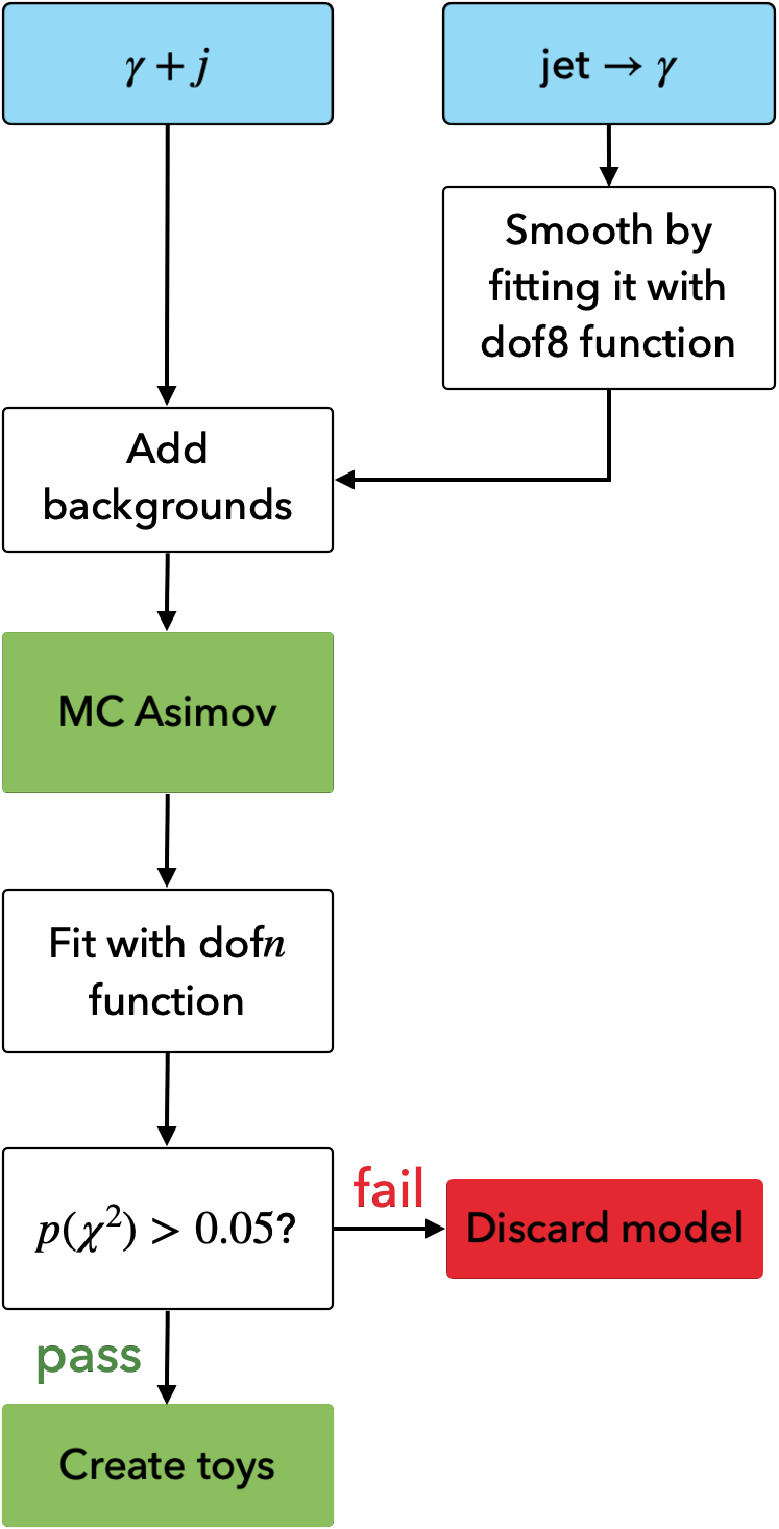
\includegraphics[width=0.3\linewidth]{5_resonances/bkg/modeling/toys_generation}
    \caption{Datasets generation for backgronud modeling studies.}
    \label{fig:bkg:modeling:preparation:datasets_generation}
\end{figure}



%%%%%%%%%%%%%%%%%%%%%%%%%%%%%%%%%%%%%%%%%%%%%%%%%%%%%%%%%%%%%%%%%%%%%%%%%%%%%%%%%%%%%%%%%%%%%%%%%%%%
\subsubsection{Smoothing of the jet-faking photon background}
\label{subsubsec:bkg:modeling:preparation:jfakes_smooth}


It was seen that approximately \(\sim 5\%\) of the \gammajet sample is populated by jet faking photon events. This background is estimated directly from data in control regions which fail calorimetric isolation (as described before), and then weighted by the corresponding \ac{FaF} as a function of \ptgam. However, specially at very high \myj, there are very few but sparse events that when they are added to the other main background (\gammajet), they distort the smooth distribution and artificial bumps start to appear, shown in \Fig{\ref{fig:bkg:modeling:preparation:jfakes_smooth:bkg_myj_distribution}}.
The jet-fakes contribution, moreover, is always an order of magnitude less than the \gammajet background.

\begin{figure}[ht!]
    \centering
    \begin{subfigure}[h]{0.49\linewidth}
        \centering
        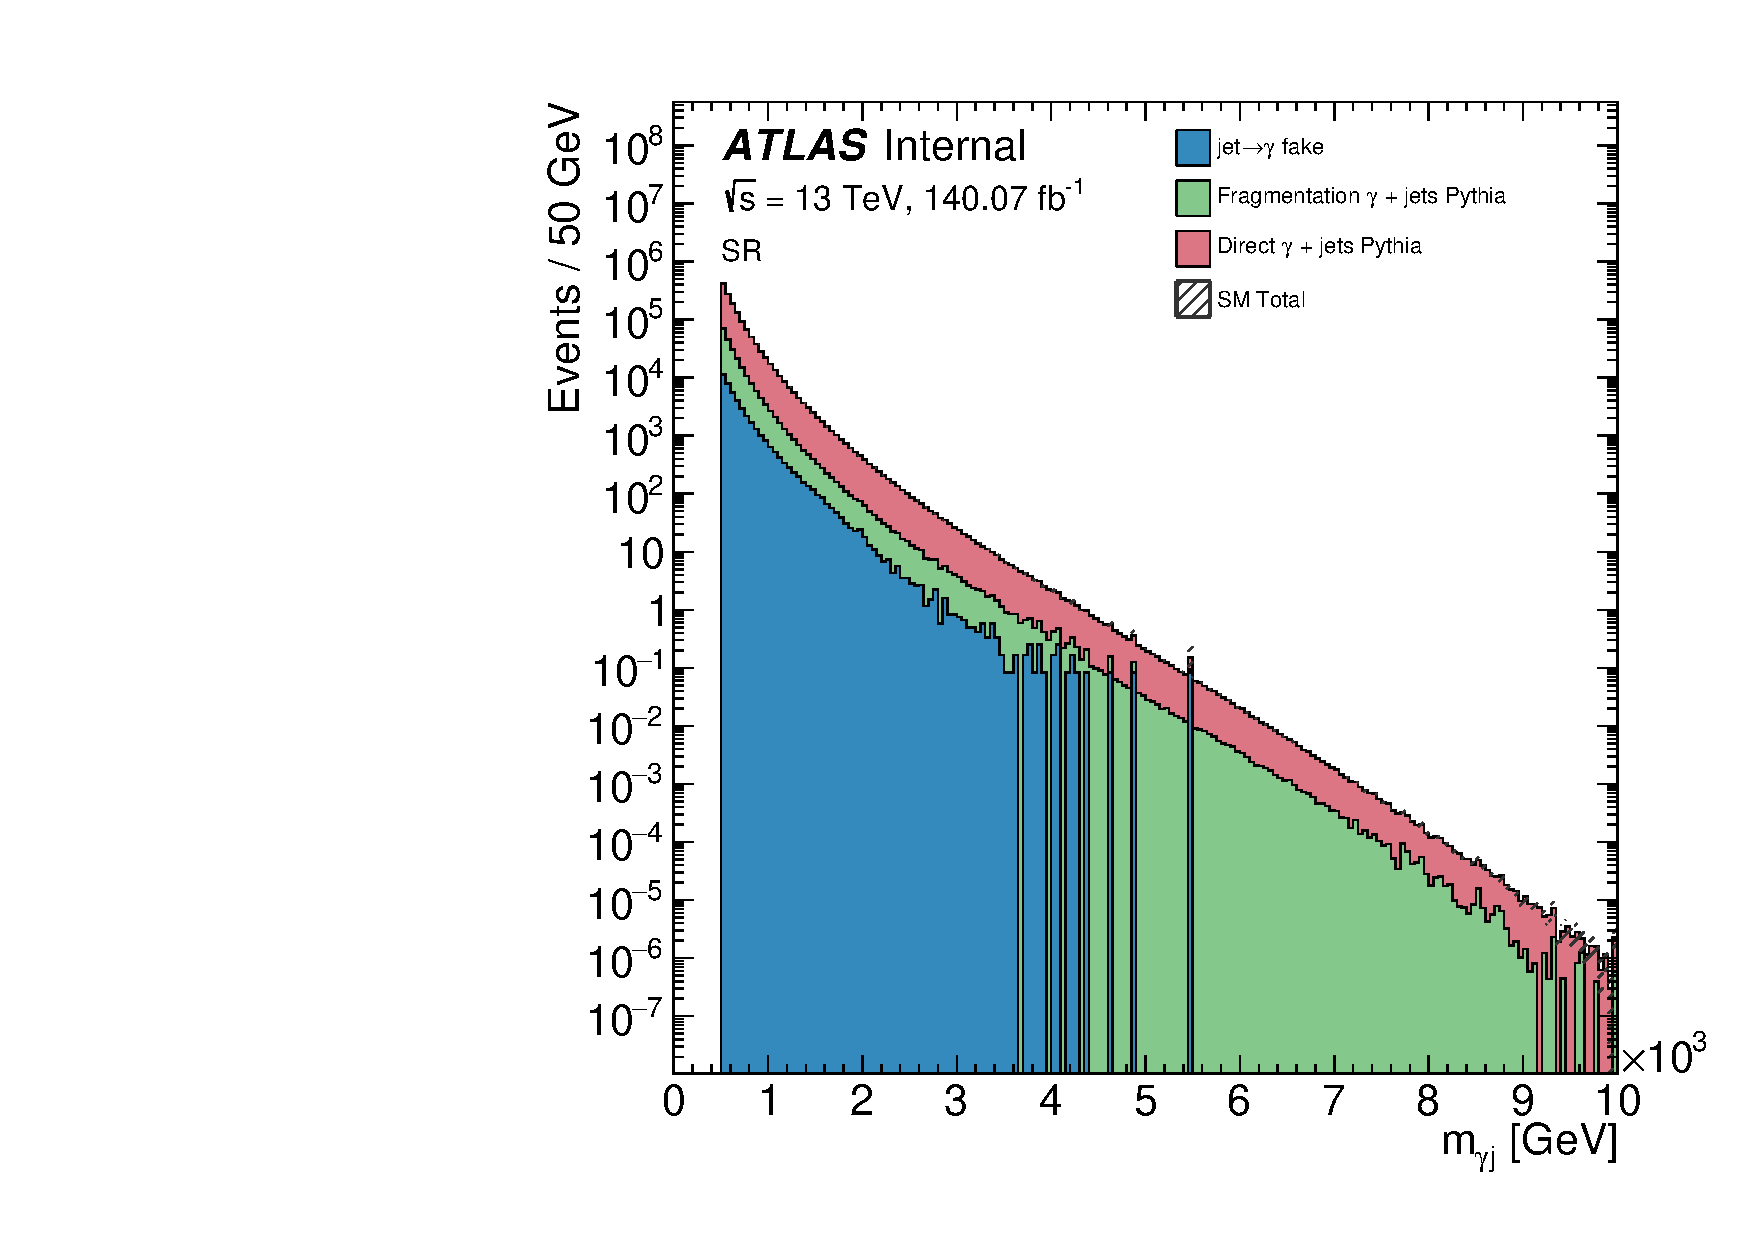
\includegraphics[width=\textwidth]{5_resonances/bkg/modeling/datasets_preparation/jfakes_smoothing/can__photonjet_Pythia_jfakeisosmooth__SR__phjet_m__Run2}
        \caption{SR}
    \end{subfigure}
    \hfill
    \begin{subfigure}[h]{0.49\linewidth}
        \centering
        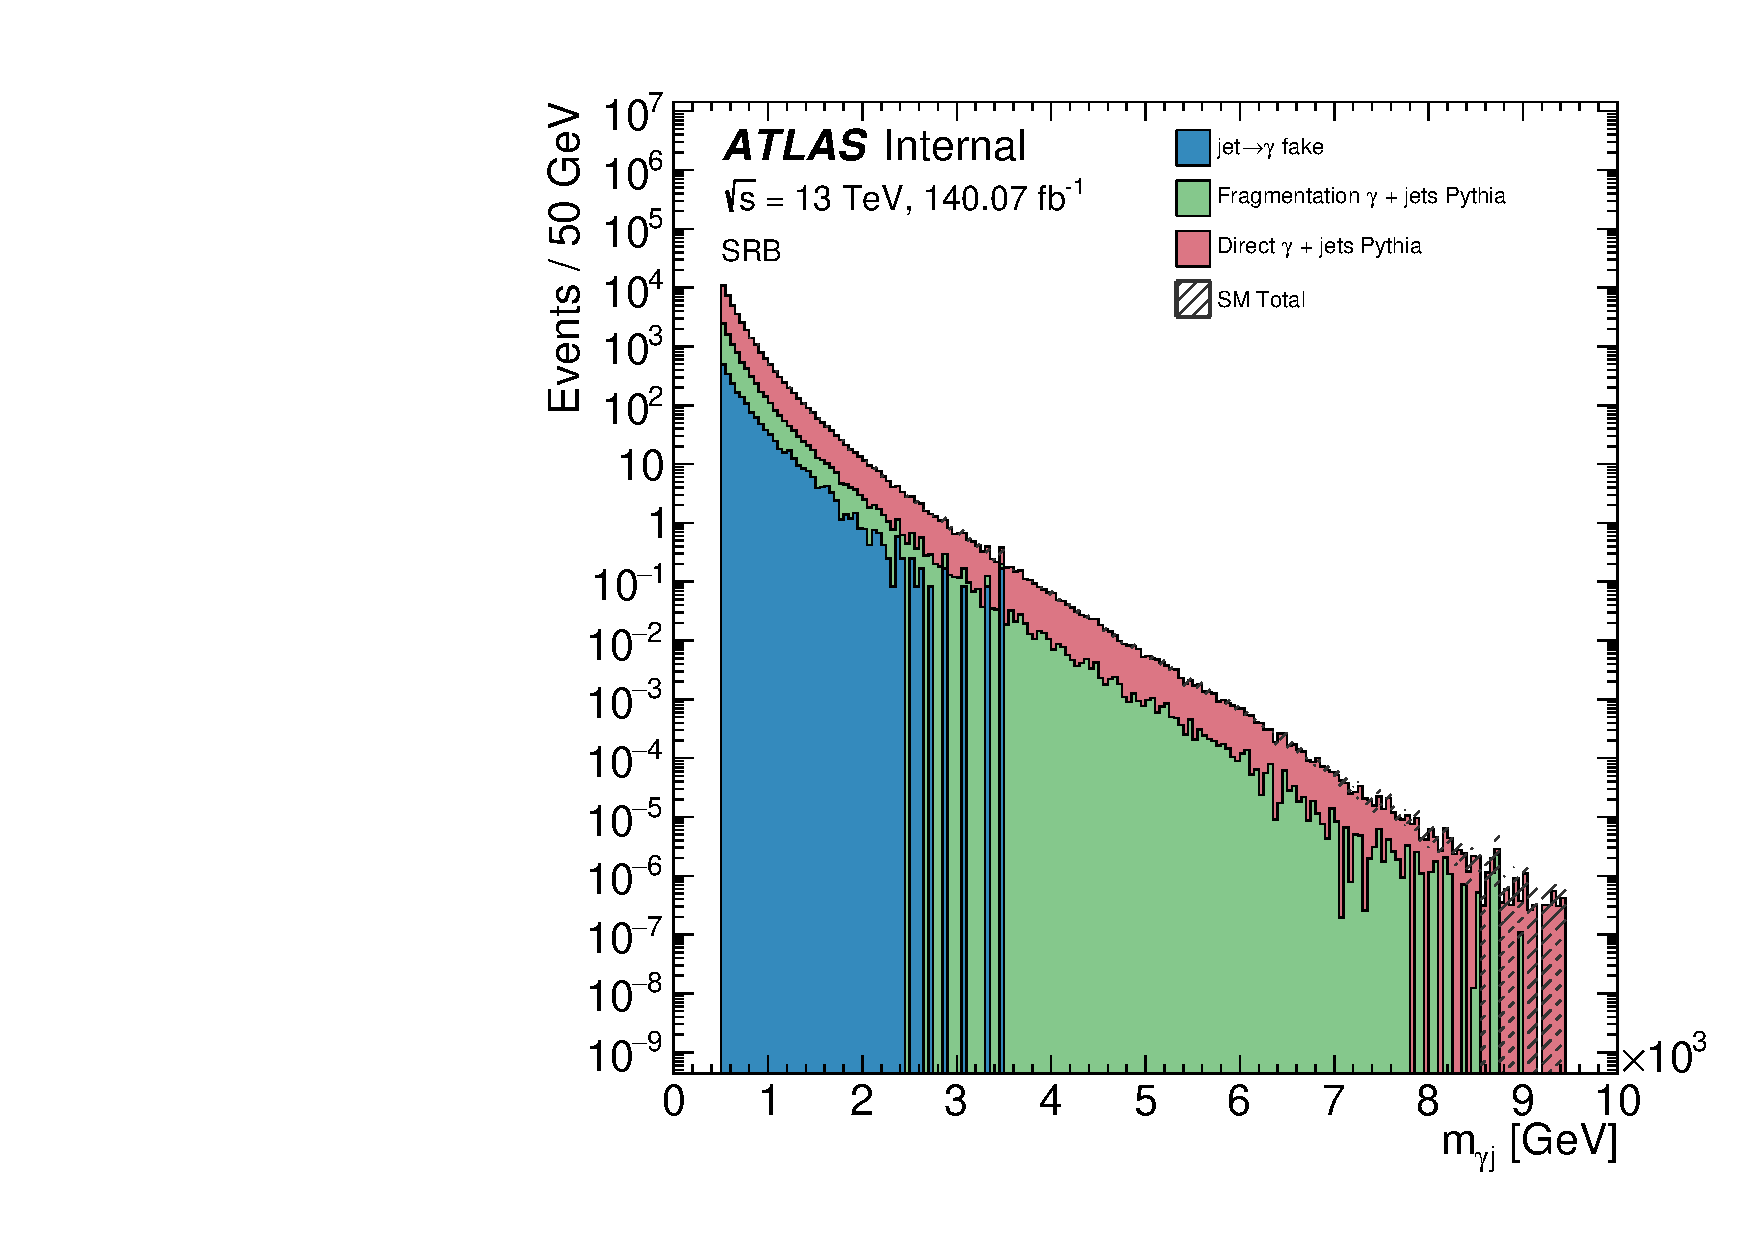
\includegraphics[width=\textwidth]{5_resonances/bkg/modeling/datasets_preparation/jfakes_smoothing/can__photonjet_Pythia_jfakeisosmooth__SRB__phjet_m__Run2}
        \caption{SRB}
    \end{subfigure}\\
    \caption{\myj distribution showing the effect of the sparsed jet-fakes events at high \myj, for the SR and SRB regions.}
    \label{fig:bkg:modeling:preparation:jfakes_smooth:bkg_myj_distribution}
\end{figure}

Taking into account these reasons, a smoothing of the jet-fakes background is performed by fitting the \myj shape with a \textit{dof8} function that will not be used to model the combined background.
The fits are done in the range \([500-10000]~\gev\), to avoid the peak of the \myj distribution. Examples of these fits for different signal regions are shown in \Fig{\ref{fig:bkg:modeling:preparation:jfakes_smooth:jfakes_fits}}, where in all cases a converged fit result is obtained.

\begin{figure}[ht!]
    \centering
    \begin{subfigure}[h]{0.49\linewidth}
        \centering
        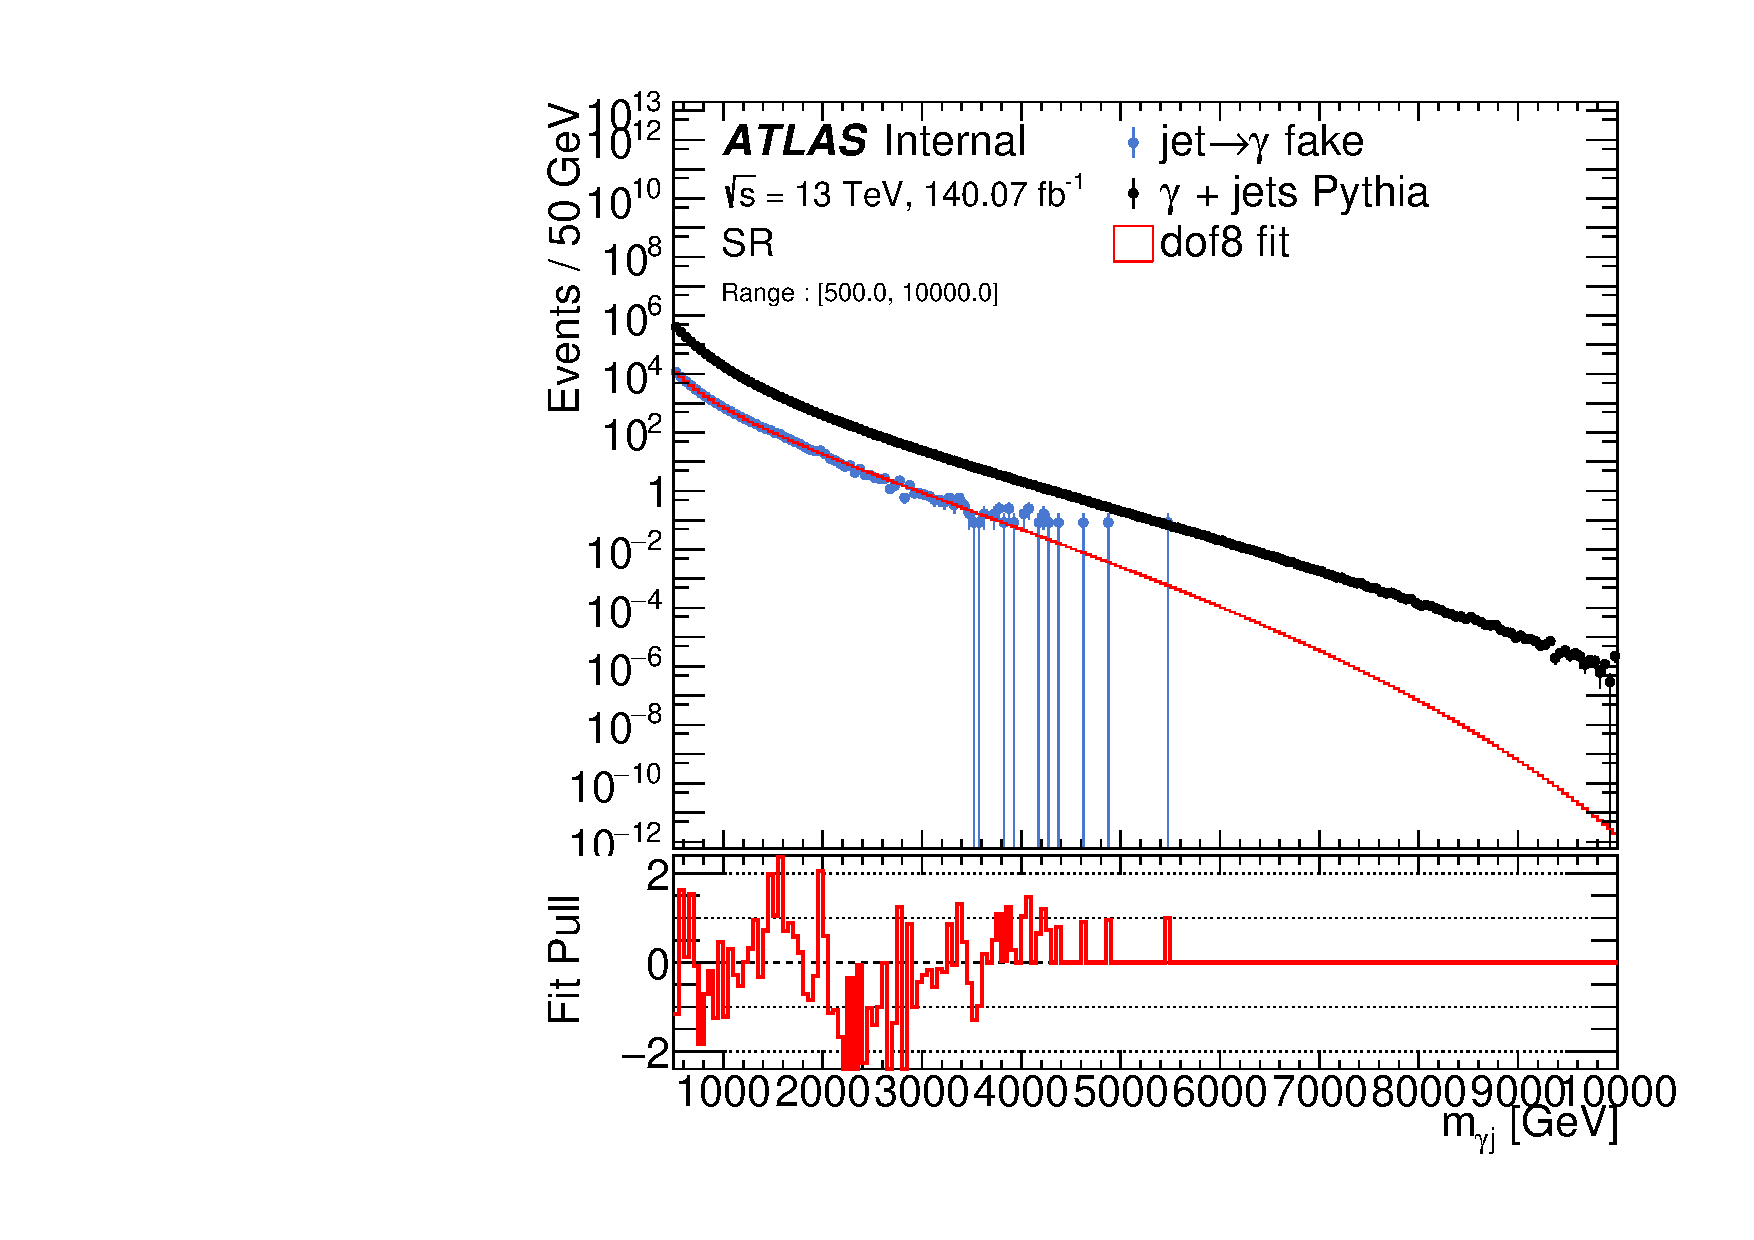
\includegraphics[width=\textwidth]{5_resonances/bkg/modeling/datasets_preparation/jfakes_smoothing/can__jfakes_fit__dof8__SR__range_500-10000}
        \caption{Inclusive SR region}
    \end{subfigure}
    \hfill
    \begin{subfigure}[h]{0.49\linewidth}
        \centering
        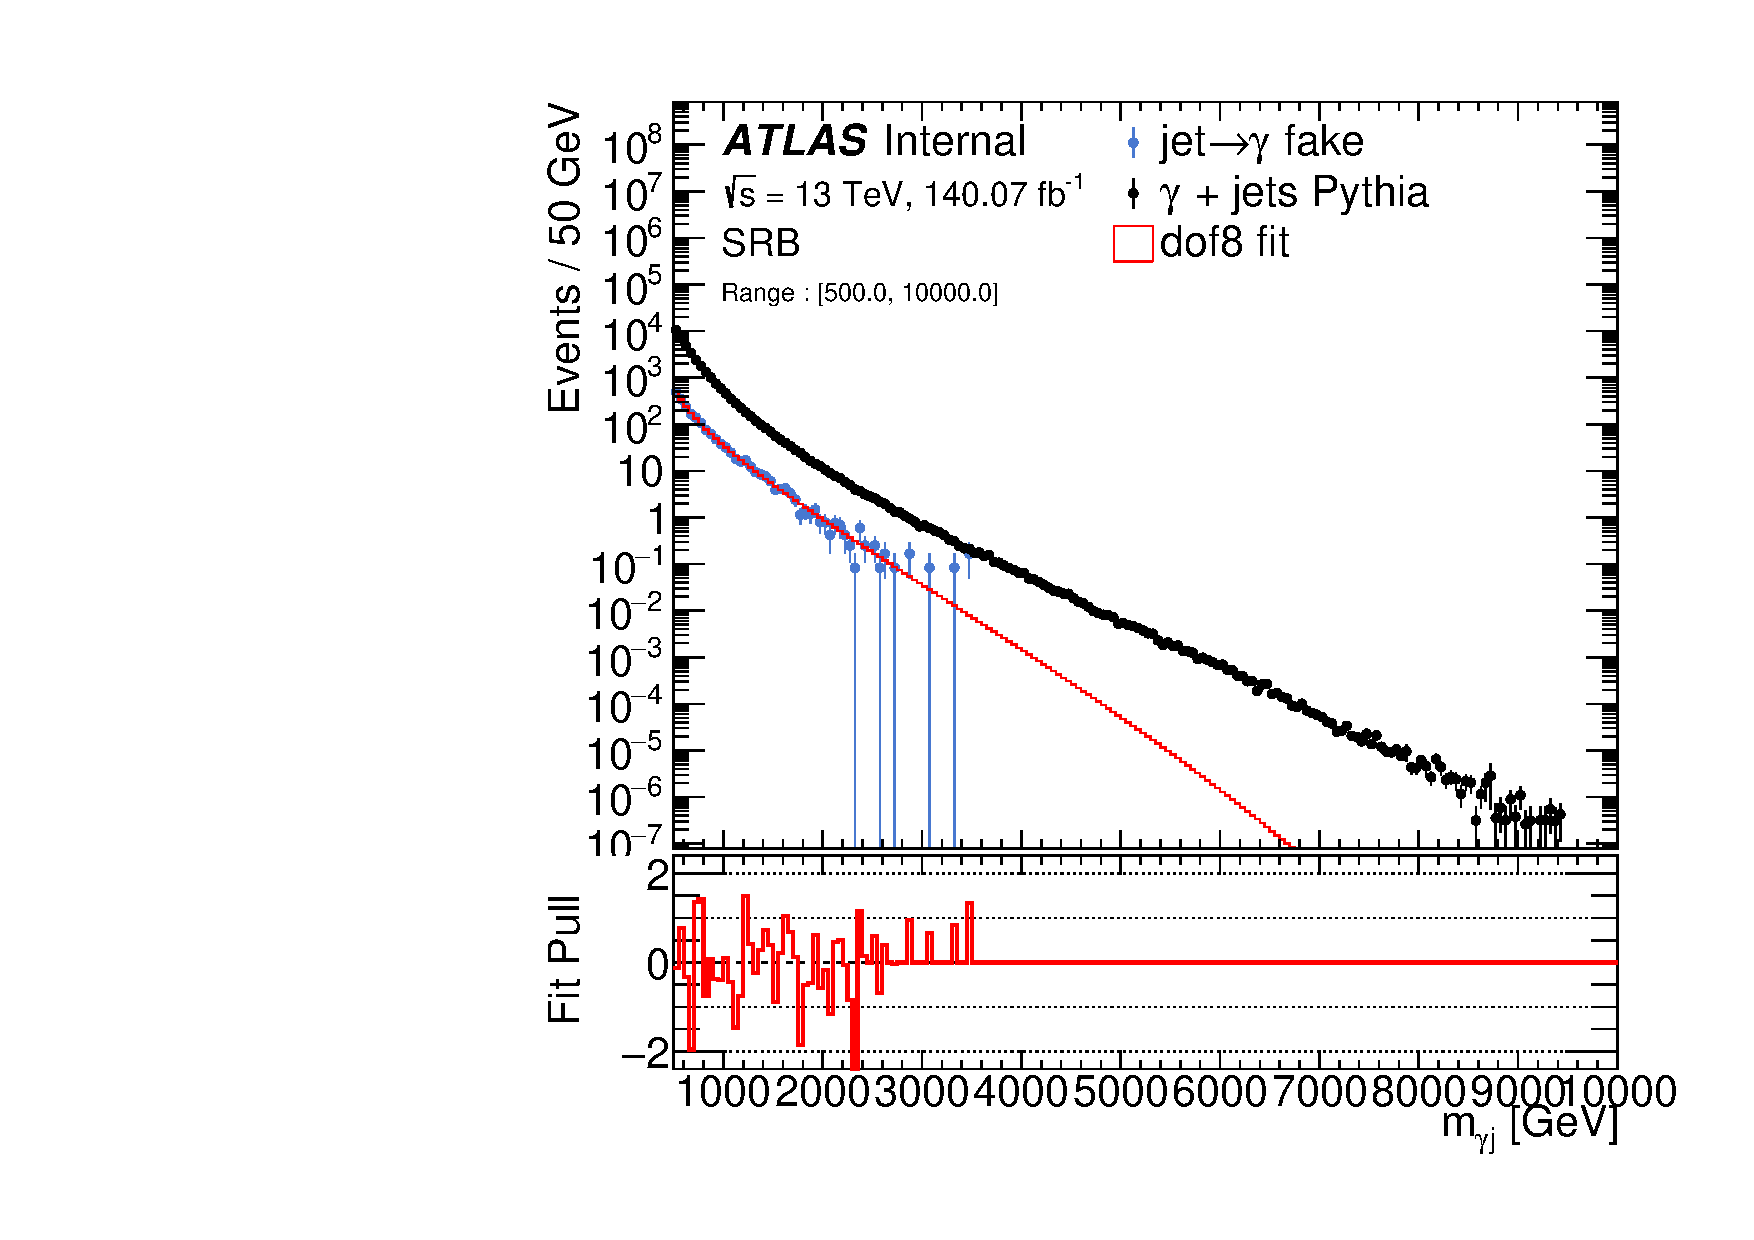
\includegraphics[width=\textwidth]{5_resonances/bkg/modeling/datasets_preparation/jfakes_smoothing/can__jfakes_fit__dof8__SRB__range_500-10000}
        \caption{\btag region, SRB}
    \end{subfigure}
    \caption{Fits to the jet-faking photons backgrounds using the \textit{dof8} functional model for different analysis regions.}
    \label{fig:bkg:modeling:preparation:jfakes_smooth:jfakes_fits}
\end{figure}


Now that the jet-faking photon background contribution is smoothed, the fit is added directly to the \ac{MC} histogram of the \gammajet background.
%%%%%%%%%%%%%%%%%%%%%%%%%%%%%%%%%%%%%%%%%%%%%%%%%%%%%%%%%%%%%%%%%%%%%%%%%%%%%%%%%%%%%%%%%%%%%%%%%%%%





%%%%%%%%%%%%%%%%%%%%%%%%%%%%%%%%%%%%%%%%%%%%%%%%%%%%%%%%%%%%%%%%%%%%%%%%%%%%%%%%%%%%%%%%%%%%%%%%%%%%
\subsubsection{Asimov datasets and background only fits}
\label{subsubsec:bkg:modeling:preparation:asimov_bkgonly}

An Asimov dataset is defined such that when one uses it to evalute the estimators for all parameters, one obtains the true parameter values:
\begin{equation}
    \hat{x} = x_0
\end{equation}
for all parameters \(x\), where \(x_0\) is the true value of the parameter. These datasets, are built as binned datasets with very fine binning, in which the event count at each bin is set to the expected event yield.

The \pythia \gammajet background benefits from large statistics, making it the best choice for a template of the \gammajet invariant mass spectrum. Therefore, the \pythia \gammajet sample, with the addition of the smoothed jet-faking photon disitribution, is fitted to create Asimov datasets. First, the bin content at each one of the bins is set to be:
\begin{equation}
    n_i = 
    \begin{cases}
        n_i, & n_i > 0\\
        0, & n_i \leq 0
    \end{cases},
\end{equation}
and bin errors set to \(\sqrt{n_i}\), where \(n_i\) is the bin content at bin \(i\).


Numerous combinations of functional models (number of \ac{dof}) and fit ranges are defined per signal region. Moreover, in order to produce toy experiments (described below) for each one of the functional models and ranges, it is important to guarantee that a simple \ac{BO} fit can be achieved with the previously created datasets.
To this end, the prepared \myj distributions are used to create Asimov datasets by fitting them with the different models, while using a big enough range to acommodate for all signals that are going to be used in the analysis in each region.

\begin{figure}[ht!]
    \centering
    \begin{subfigure}[h]{0.32\linewidth}
        \centering
        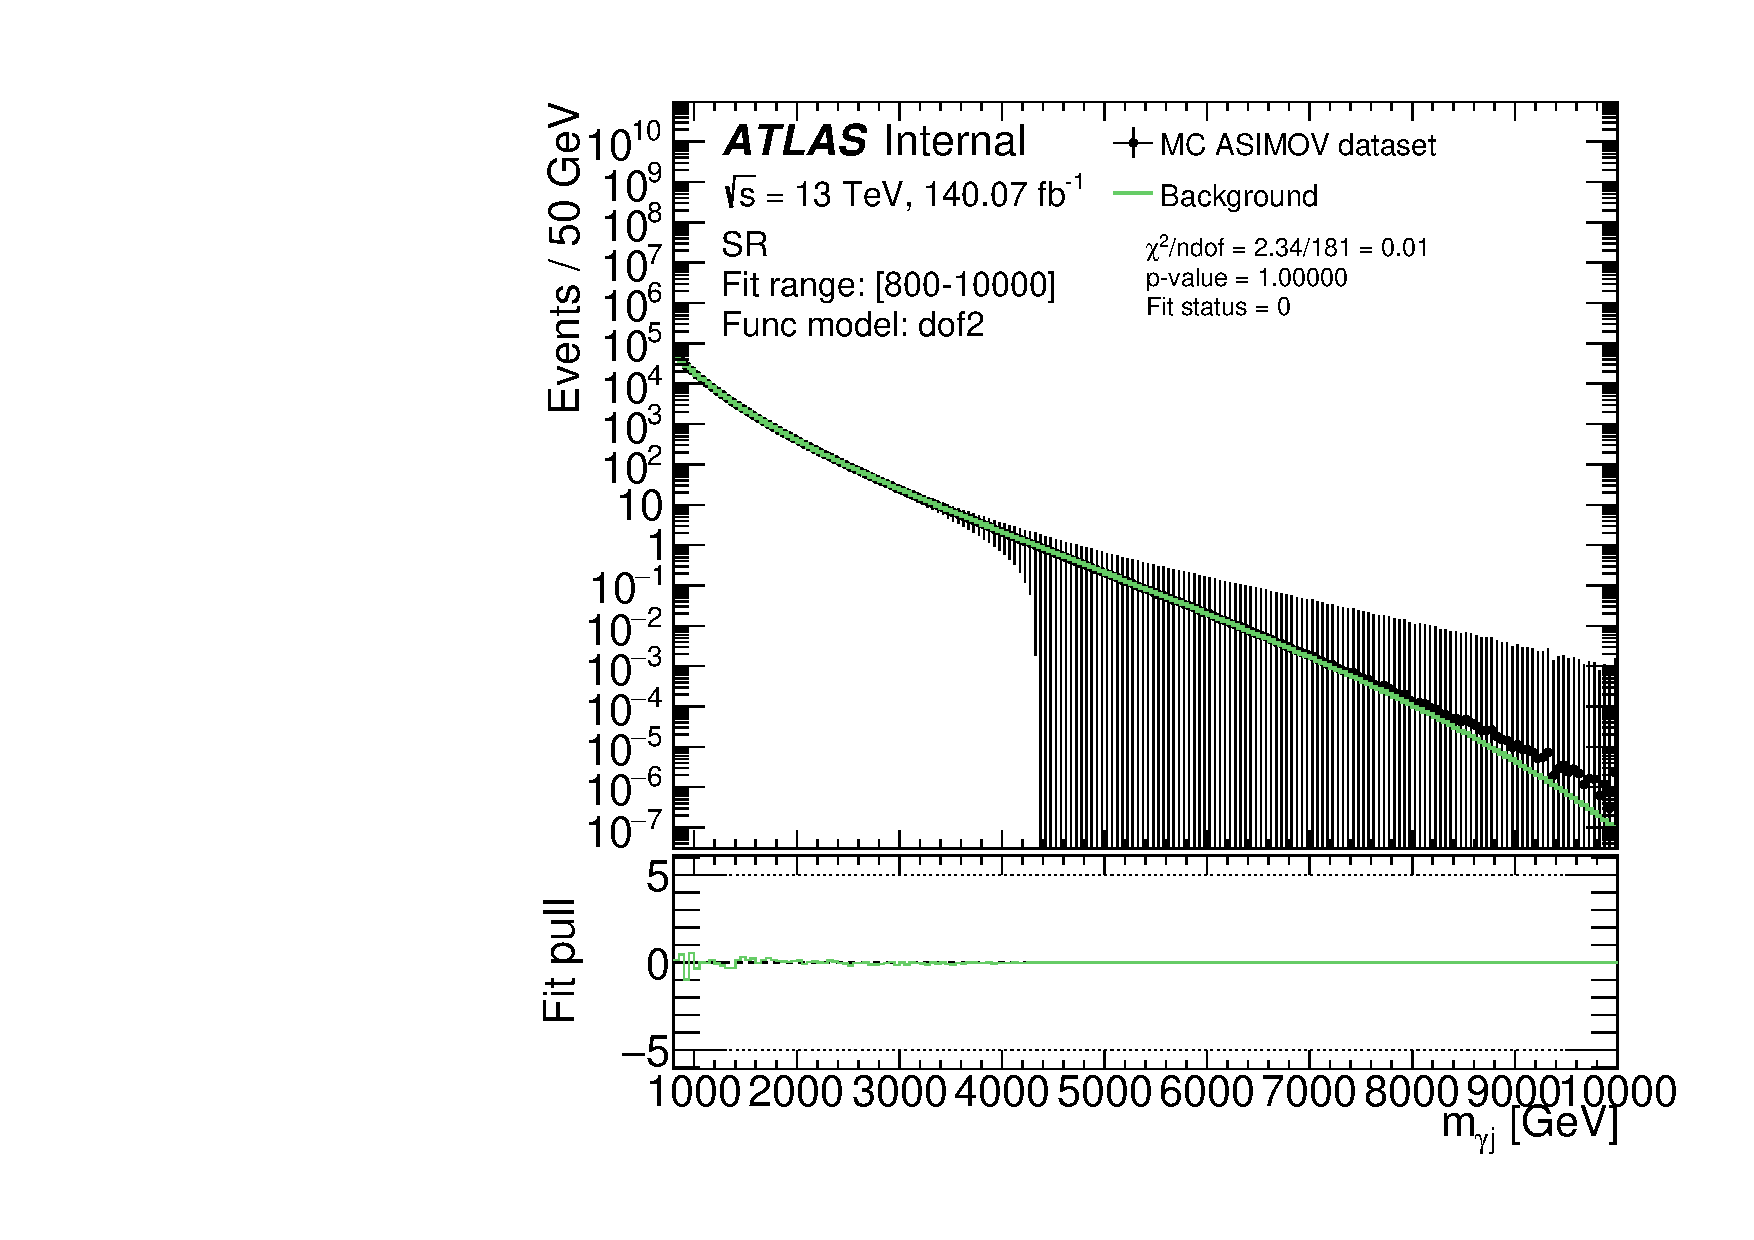
\includegraphics[width=\textwidth]{5_resonances/bkg/modeling/datasets_preparation/fit_hists/SR/can__bkgonlyfit__asimov__photonjet_Pythia__SR__dof2__range_800-10000}
    \end{subfigure}
    \hfill
    \begin{subfigure}[h]{0.32\linewidth}
        \centering
        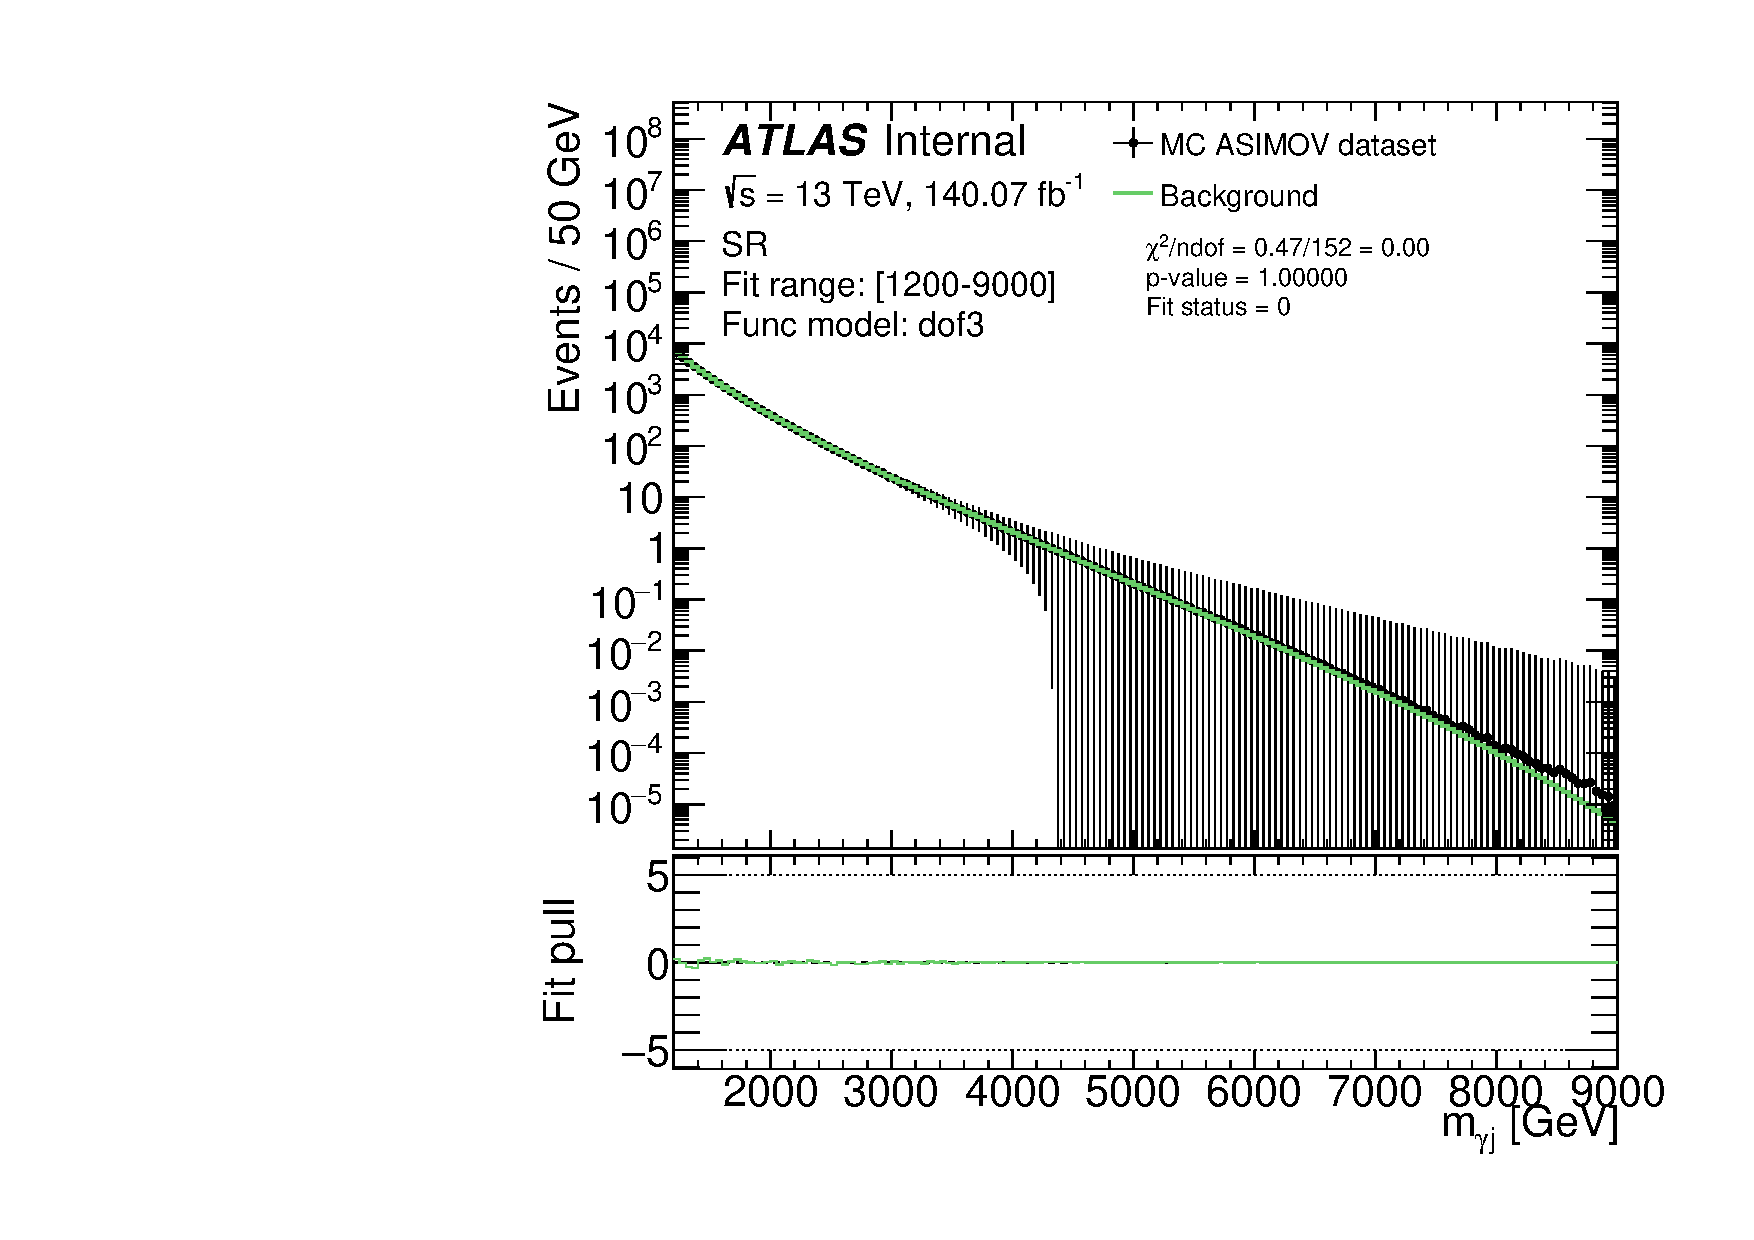
\includegraphics[width=\textwidth]{5_resonances/bkg/modeling/datasets_preparation/fit_hists/SR/can__bkgonlyfit__asimov__photonjet_Pythia__SR__dof3__range_1200-9000}
    \end{subfigure}
    \hfill
    \begin{subfigure}[h]{0.32\linewidth}
        \centering
        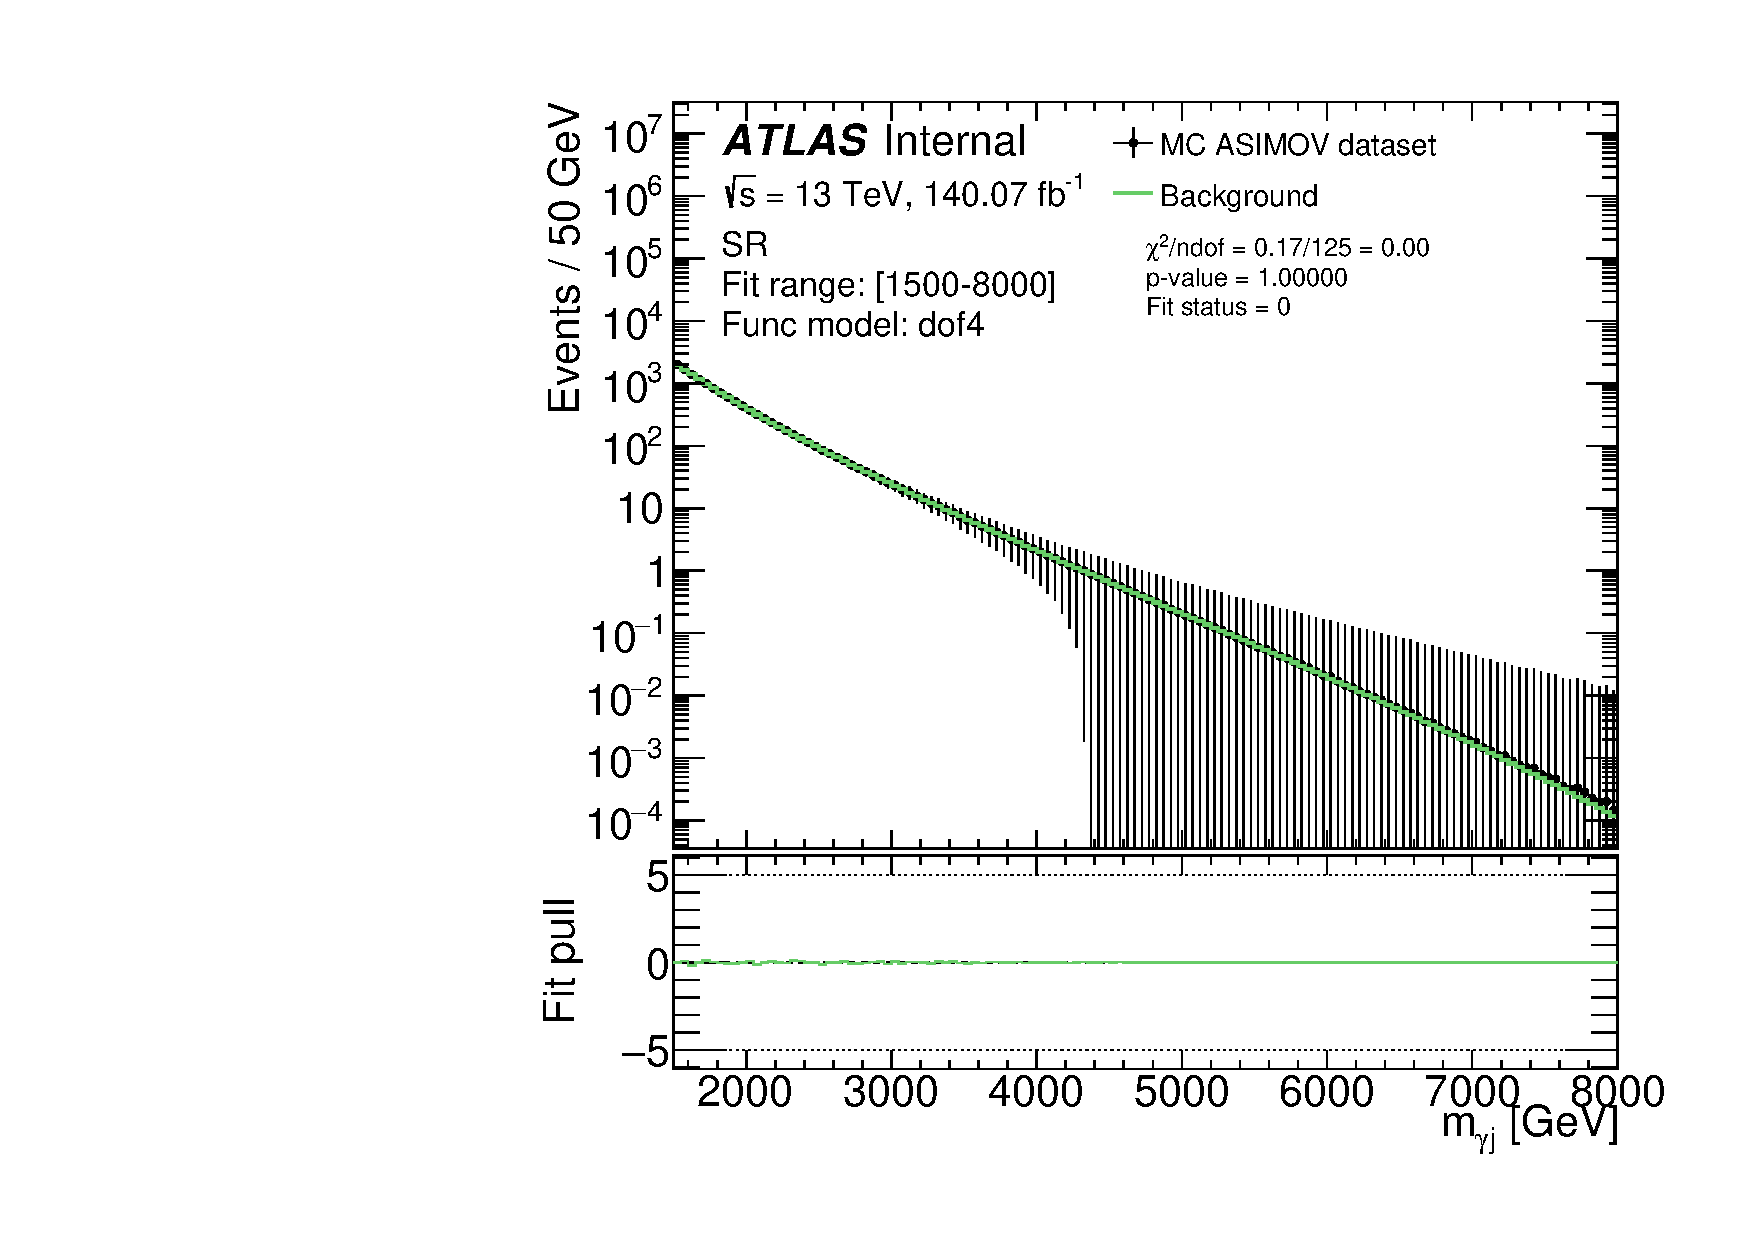
\includegraphics[width=\textwidth]{5_resonances/bkg/modeling/datasets_preparation/fit_hists/SR/can__bkgonlyfit__asimov__photonjet_Pythia__SR__dof4__range_1500-8000}
    \end{subfigure}\\
    \caption{Background only fits using different functional models and fit ranges for the inclusive SR region.}
    \label{fig:bkg:modeling:preparation:asimov_bkgonly:bkgonly_fits}
\end{figure}

\Fig{\ref{fig:bkg:modeling:preparation:asimov_bkgonly:bkgonly_fits}} shows some examples of \ac{BO} fits done in the inclusive SR. As it can be seen, all functions succeed to represent the background distribution.
% The same combinations of fit-ranges and functional models are shown in \App{\ref{app:bkgonly_fits:bkgonly_fits_asimov}} for other signal regions.
%%%%%%%%%%%%%%%%%%%%%%%%%%%%%%%%%%%%%%%%%%%%%%%%%%%%%%%%%%%%%%%%%%%%%%%%%%%%%%%%%%%%%%%%%%%%%%%%%%%%





%%%%%%%%%%%%%%%%%%%%%%%%%%%%%%%%%%%%%%%%%%%%%%%%%%%%%%%%%%%%%%%%%%%%%%%%%%%%%%%%%%%%%%%%%%%%%%%%%%%%
\subsubsection{Pseudo-data generation}
\label{subsubsec:bkg:modeling:preparation:toys}

Pseudo-data, or also called \textit{toys} distributions, are essentialy background distributions used to mimic real data. Toys are computed from \ac{BO} fits to the Asimov datasets, and each bin of the distribution is computed as a Poisson random number with mean \(v_i = n_i\), where \(n_i\) is the fit evaluated at bin \(i\). Different sets of toys distributions are computed depending on the number of parameters the \ac{BO} fit has been made. A total of 500 toys are generated per signal region and per functional model.

To test fits using the \textit{dofn} model, pseudo-data distributions generated from a \textit{dof(n+1)} model are used. In \Fig{\ref{fig:bkg:modeling:preparation:toys:bkgonly_examples_toys_fits}}, two fit examples to toys are shown. In this case, the toys were generated from a \textit{dof3} fit to the MC, and are now being fitted with a \textit{dof2} model.

\begin{figure}[ht!]
    \centering
    \begin{subfigure}[h]{0.49\linewidth}
        \centering
        \includegraphics[width=\textwidth, page=123]{5_resonances/bkg/modeling/datasets_preparation/fit_toys/SR/dof2__range_800-10000/can__bkgonlyfit__toys__photonjet_Pythia__SR__dof2__range_800-10000}
    \end{subfigure}
    \hfill
    \begin{subfigure}[h]{0.49\linewidth}
        \centering
        \includegraphics[width=\textwidth, page=432]{5_resonances/bkg/modeling/datasets_preparation/fit_toys/SR/dof2__range_800-10000/can__bkgonlyfit__toys__photonjet_Pythia__SR__dof2__range_800-10000}
    \end{subfigure}\\
    \caption{\ac{BO} fits to different toys in the SR region}
    \label{fig:bkg:modeling:preparation:toys:bkgonly_examples_toys_fits}
\end{figure}

\begin{figure}[ht!]
    \centering
    \begin{subfigure}[h]{0.32\linewidth}
        \centering
        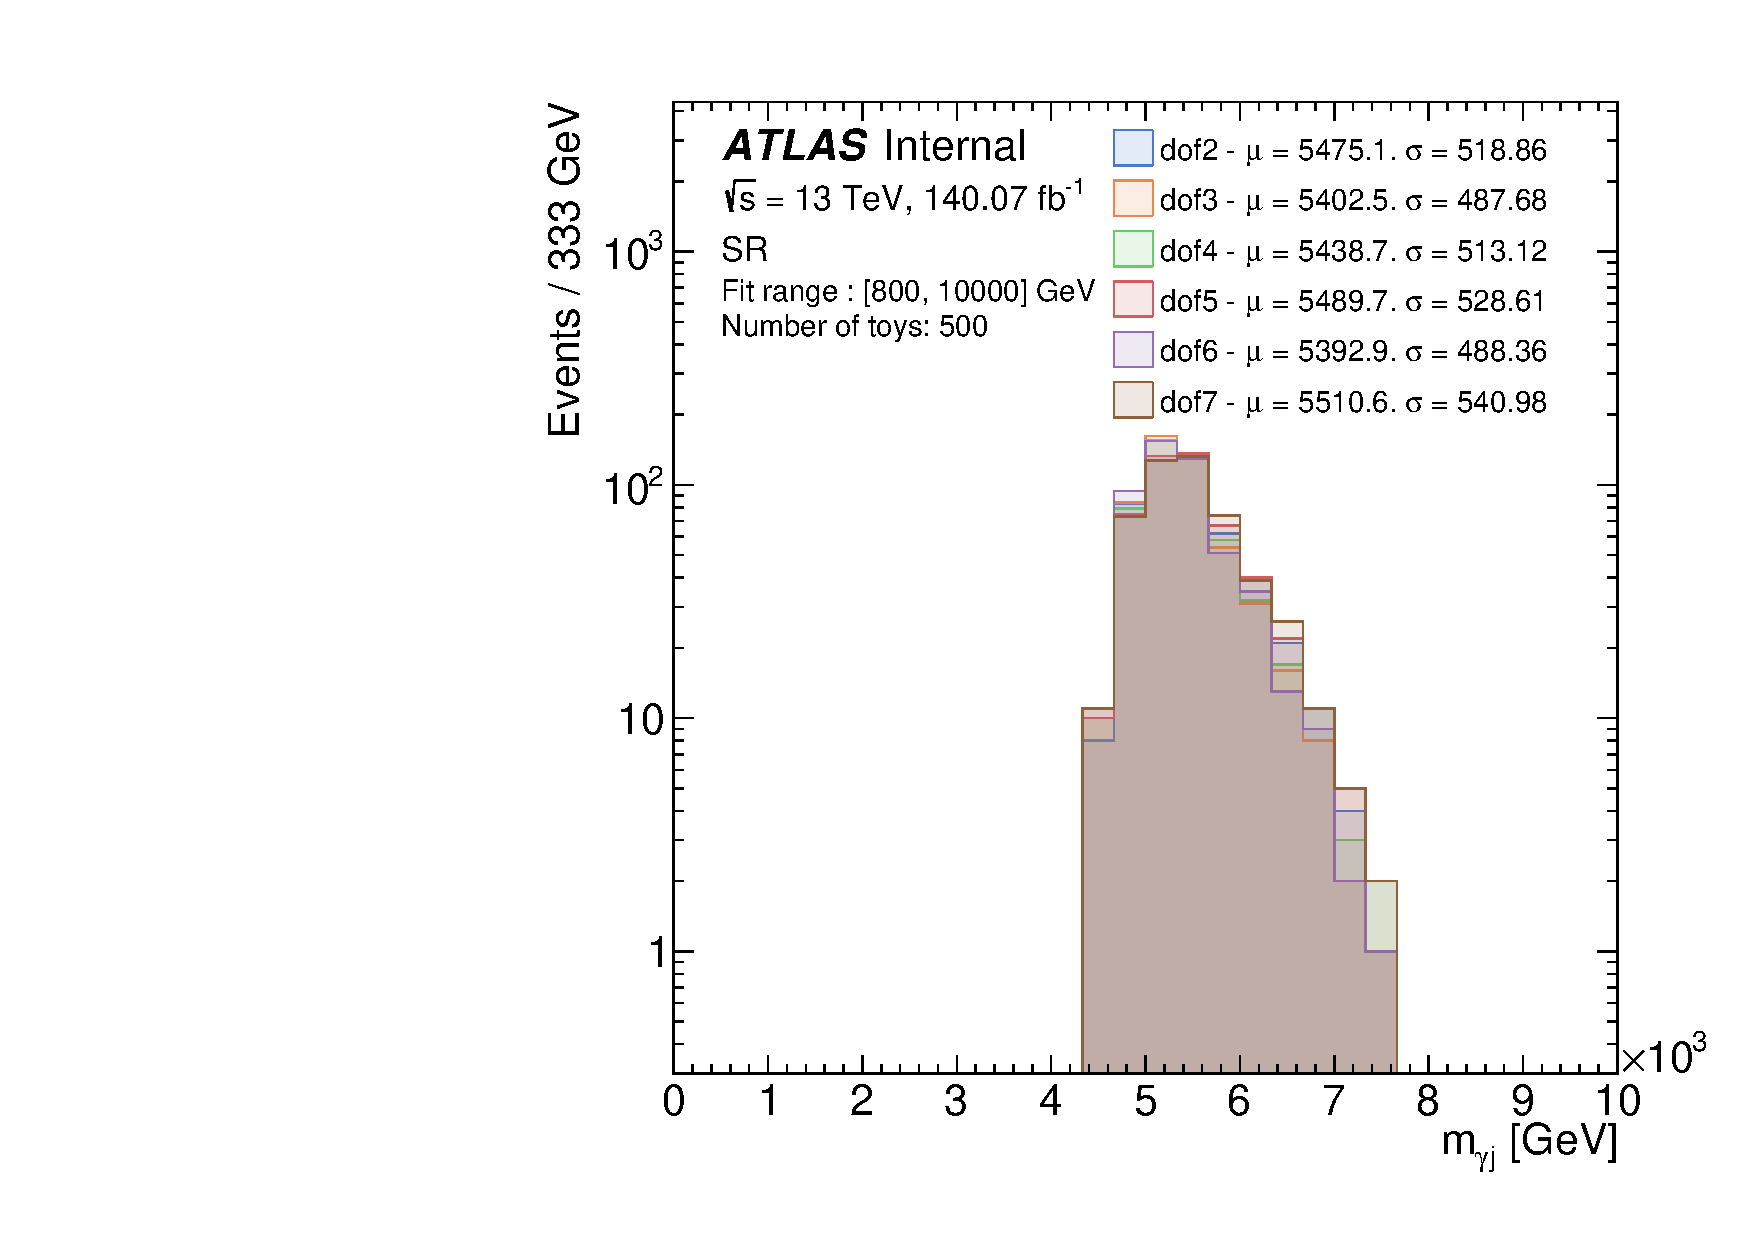
\includegraphics[width=\textwidth]{5_resonances/bkg/modeling/datasets_preparation/fit_toys/maximums/can__bkgPythia__SR__range_800_10000__phjet_m__toys_maximum}
        \caption{SR}
    \end{subfigure}\\
    \begin{subfigure}[h]{0.32\linewidth}
        \centering
        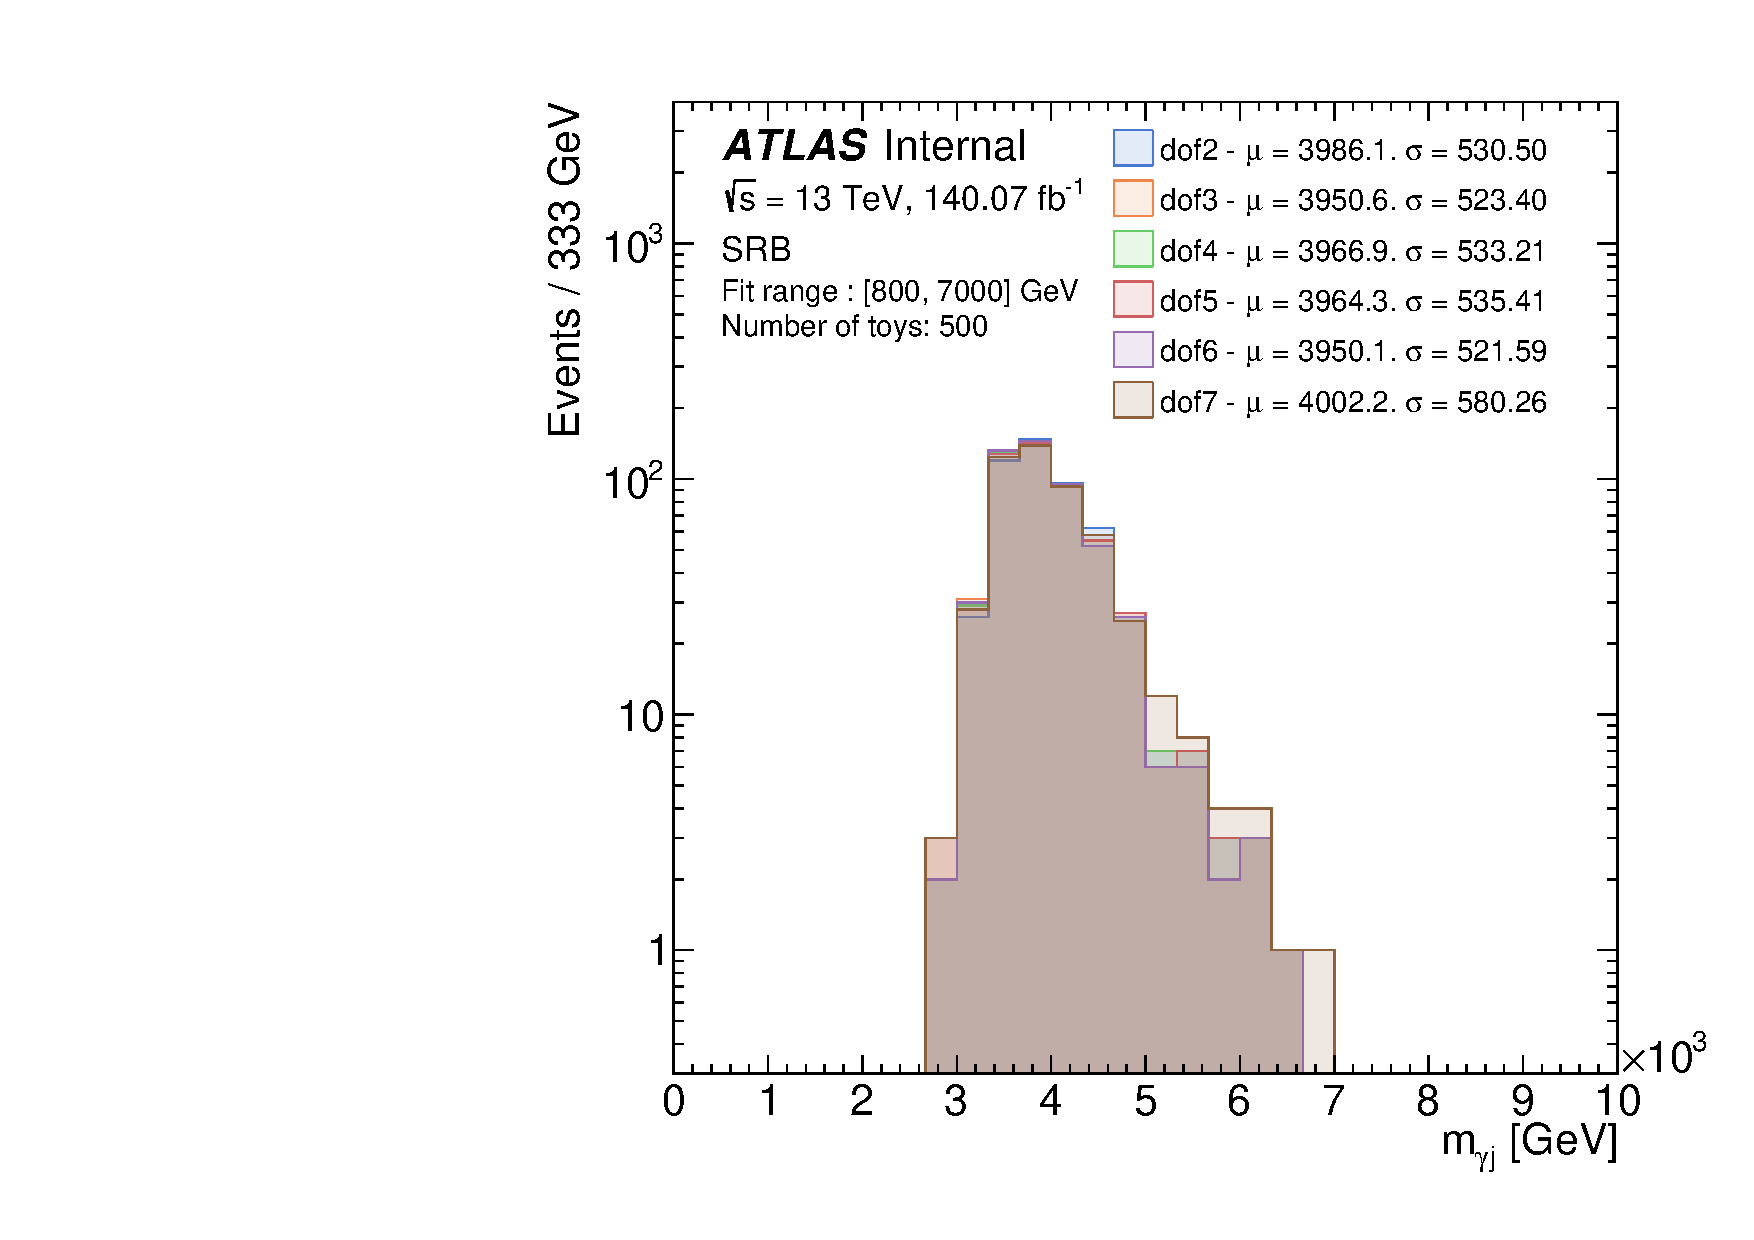
\includegraphics[width=\textwidth]{5_resonances/bkg/modeling/datasets_preparation/fit_toys/maximums/can__bkgPythia__SRB__range_800_7000__phjet_m__toys_maximum}
        \caption{SRB}
    \end{subfigure}
    \begin{subfigure}[h]{0.32\linewidth}
        \centering
        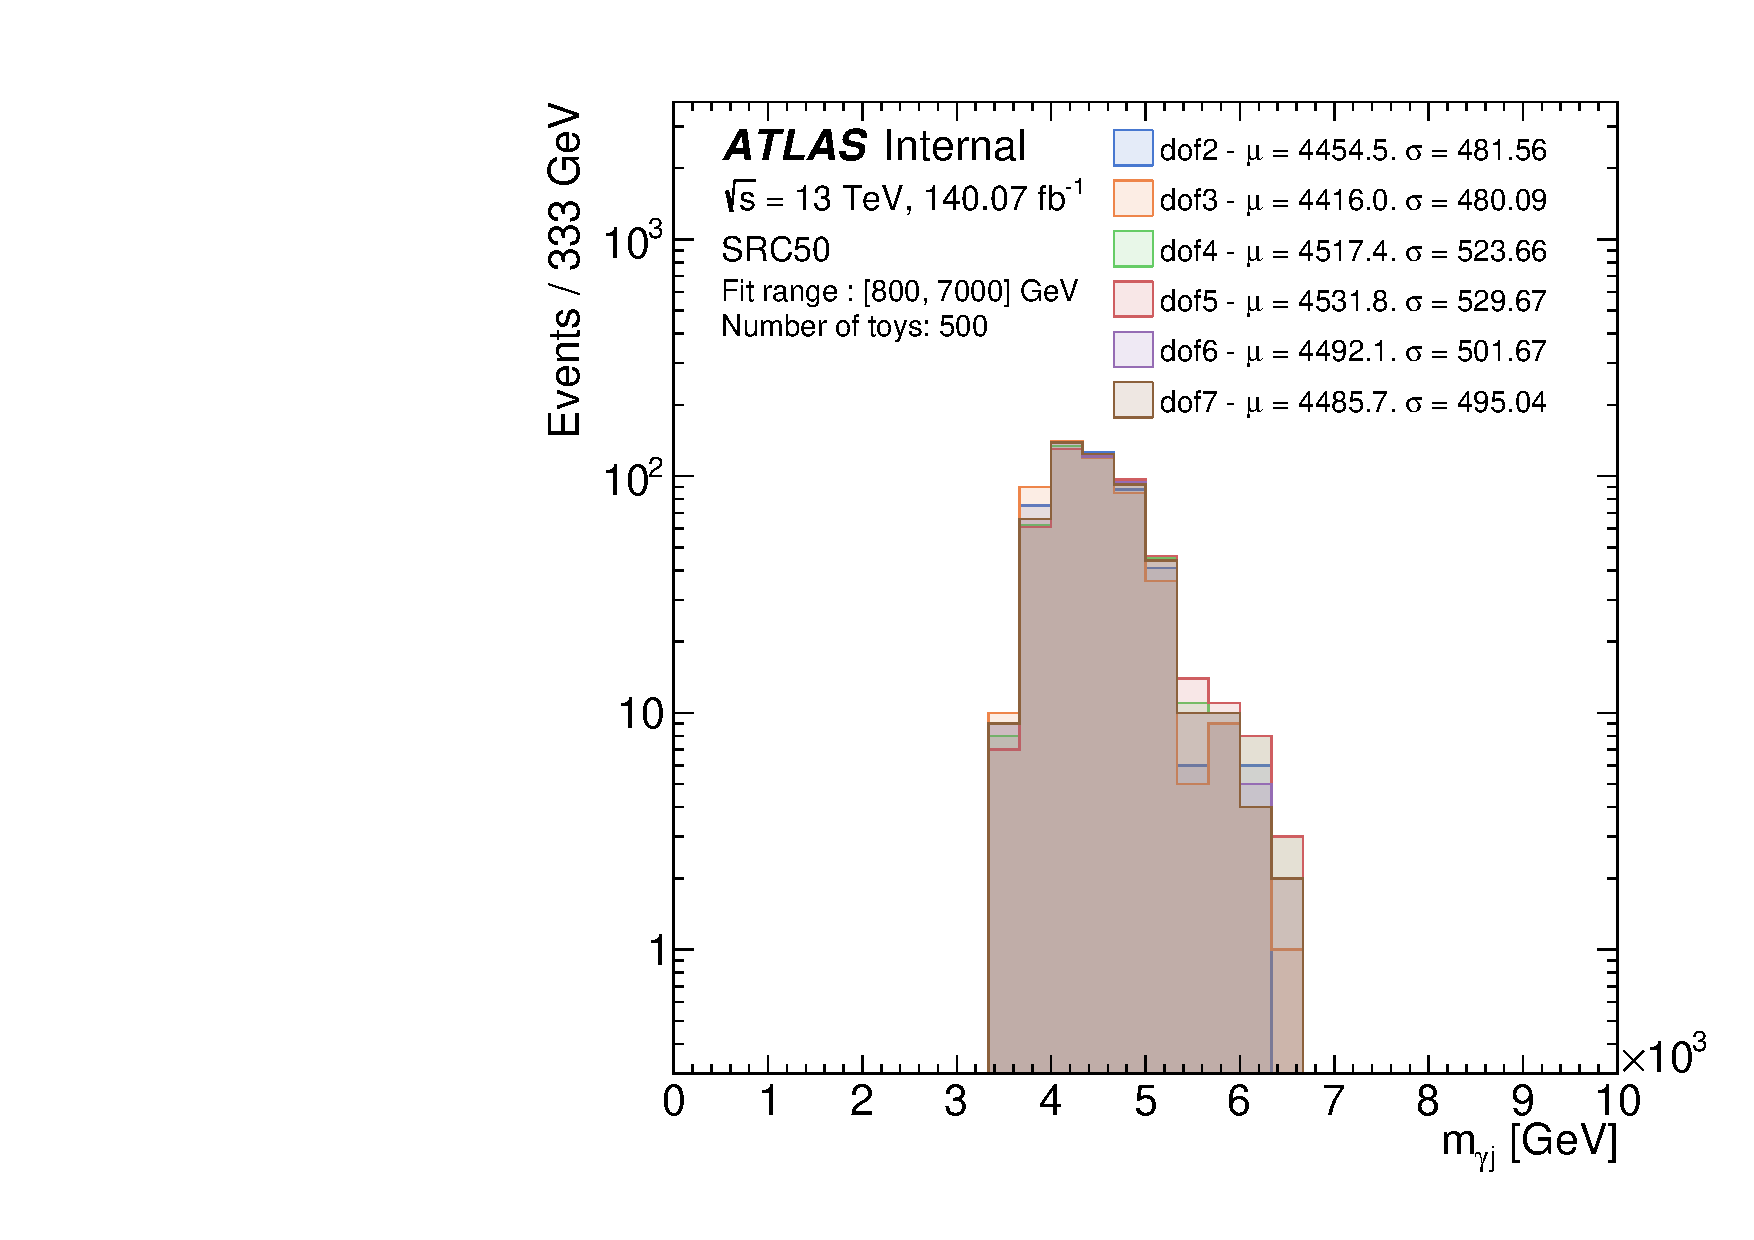
\includegraphics[width=\textwidth]{5_resonances/bkg/modeling/datasets_preparation/fit_toys/maximums/can__bkgPythia__SRC50__range_800_7000__phjet_m__toys_maximum}
        \caption{SRC}
    \end{subfigure}
    \begin{subfigure}[h]{0.32\linewidth}
        \centering
        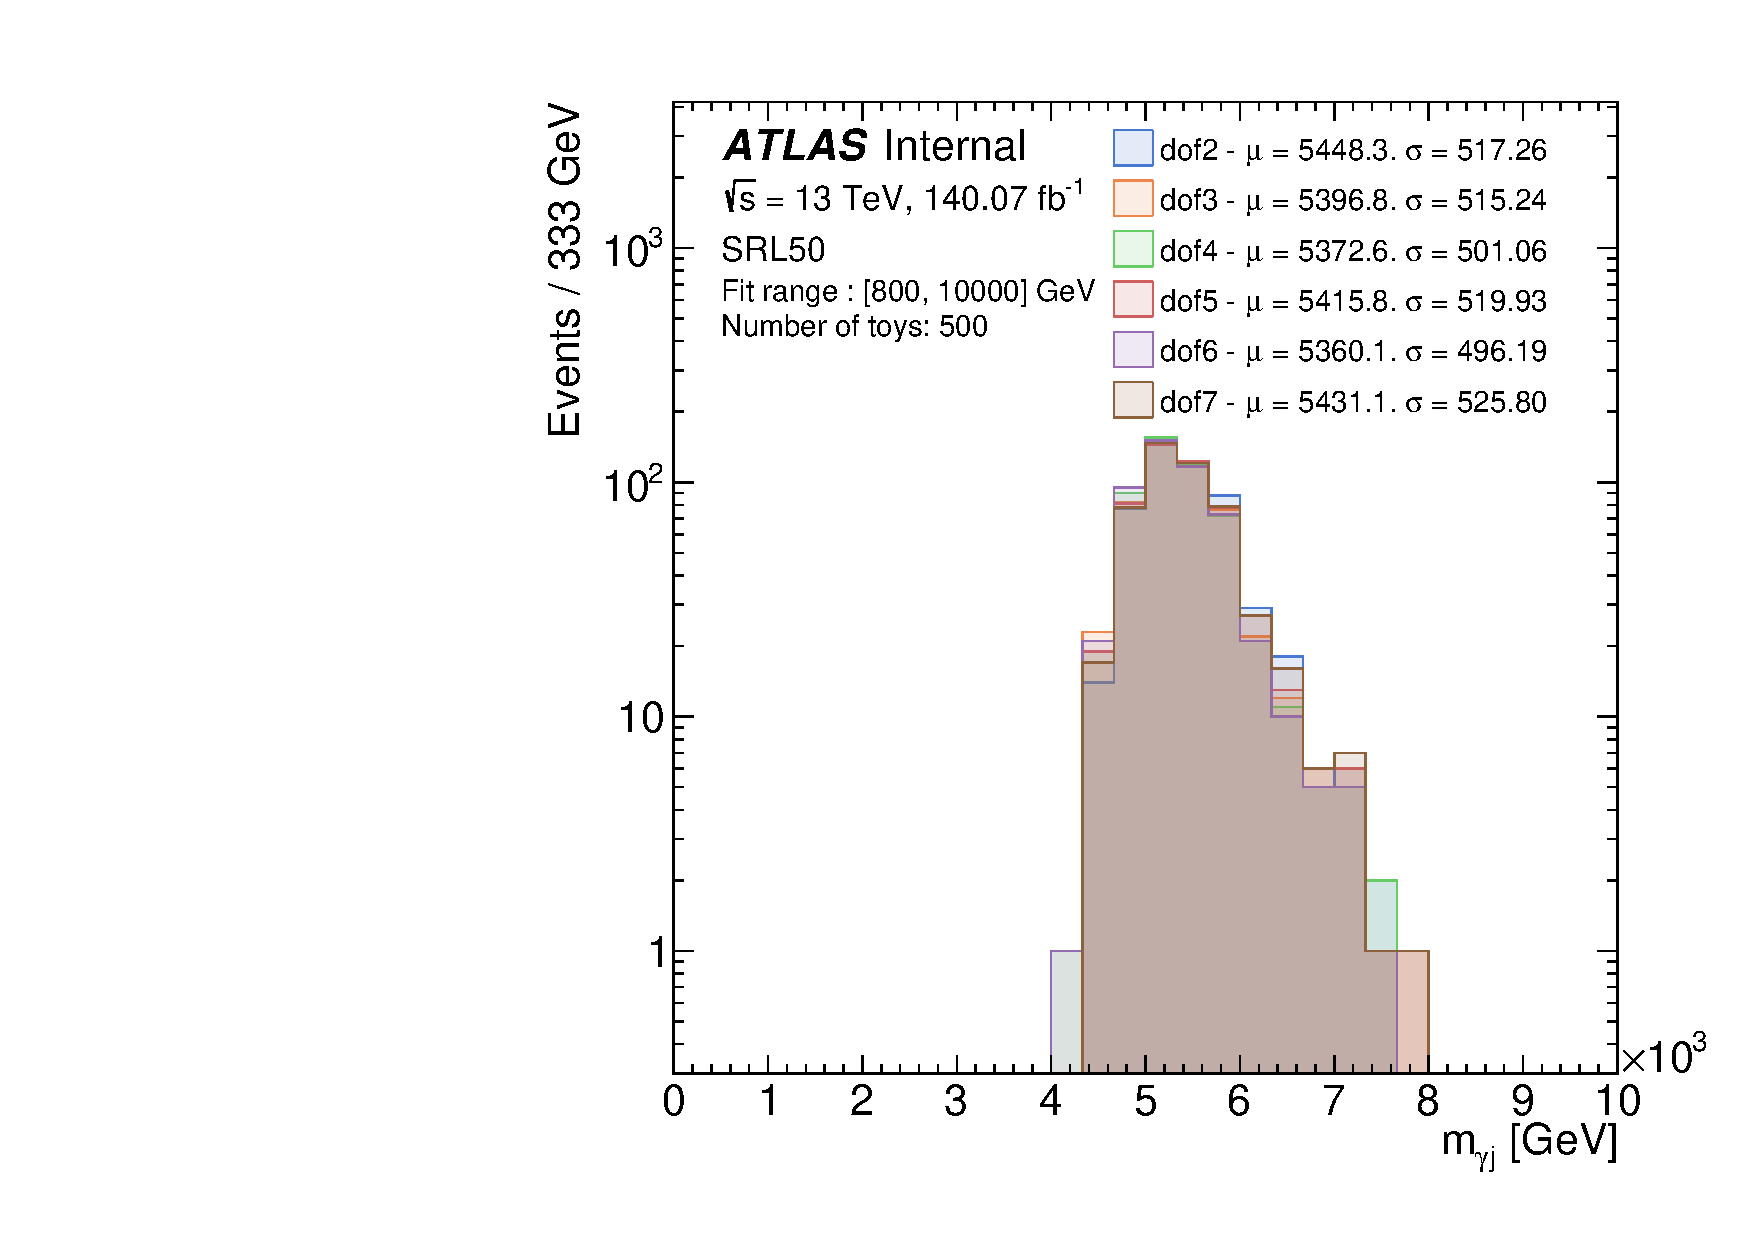
\includegraphics[width=\textwidth]{5_resonances/bkg/modeling/datasets_preparation/fit_toys/maximums/can__bkgPythia__SRL50__range_800_10000__phjet_m__toys_maximum}
        \caption{SRL}
    \end{subfigure}\\
    \caption{\myj maximum distribution for the toys sets for each signal region considered. The different sets of toys, corresponding to different initial \textit{dofn} functions, are shown with different colors. For each one of them, the mean and the width of the distribution is shown.}
    \label{fig:bkg:modeling:preparation:toys:toys_maximums}
\end{figure}

As previously stated, toys distributions are made to mimic the behaviour real data would have. In order to have a first guess on the maximum \myj value that can be obtained from data, in \Fig{\ref{fig:bkg:modeling:preparation:toys:toys_maximums}} the maximum \myj value distribution is shown, for each set of toy generated from the different functional models. For any of the regions dominated by \ljets, the last toy event is approximately at \(\sim 5500~\gev\) and the right tails extends up to \(\sim 8000~\gev\). Similarly, for the \cjets and \bjets regions, there are toy events up to \(\sim 6~\tev\), with the mean at \(\sim 4~\tev\). For these reasons, it is important that the upper limit on the fit-ranges are always higher than the last present event.
%%%%%%%%%%%%%%%%%%%%%%%%%%%%%%%%%%%%%%%%%%%%%%%%%%%%%%%%%%%%%%%%%%%%%%%%%%%%%%%%%%%%%%%%%%%%%%%%%%%%

%%%%%%%%%%%%%%%%%%%%%%%%%%%%%%%%%%%%%%%%%%%%%%%%%%%%%%%%%%%%%%%%%%%%%%%%%%%%%%%%%%%%%%%%%%%%%%%%%%%%
%%%%%%%%%%%%%%%%%%%%%%%%%%%%%%%%%%%%%%%%%%%%%%%%%%%%%%%%%%%%%%%%%%%%%%%%%%%%%%%%%%%%%%%%%%%%%%%%%%%%
%%%%%%%%%%%%%%%%%%%%%%%%%%%%%%%%%%%%%%%%%%%%%%%%%%%%%%%%%%%%%%%%%%%%%%%%%%%%%%%%%%%%%%%%%%%%%%%%%%%%
















%%%%%%%%%%%%%%%%%%%%%%%%%%%%%%%%%%%%%%%%%%%%%%%%%%%%%%%%%%%%%%%%%%%%%%%%%%%%%%%%%%%%%%%%%%%%%%%%%%%%
%%%%%%%%%%%%%%%%%%%%%%%%%%%%%%%%%%%%%%%%%%%%%%%%%%%%%%%%%%%%%%%%%%%%%%%%%%%%%%%%%%%%%%%%%%%%%%%%%%%%
%%%%%%%%%%%%%%%%%%%%%%%%%%%%%%%%%%%%%%%%%%%%%%%%%%%%%%%%%%%%%%%%%%%%%%%%%%%%%%%%%%%%%%%%%%%%%%%%%%%%
\subsection{Modeling strategy}
\label{subsec:bkg:modeling:strategy}


\begin{figure}[ht!]
    \centering
    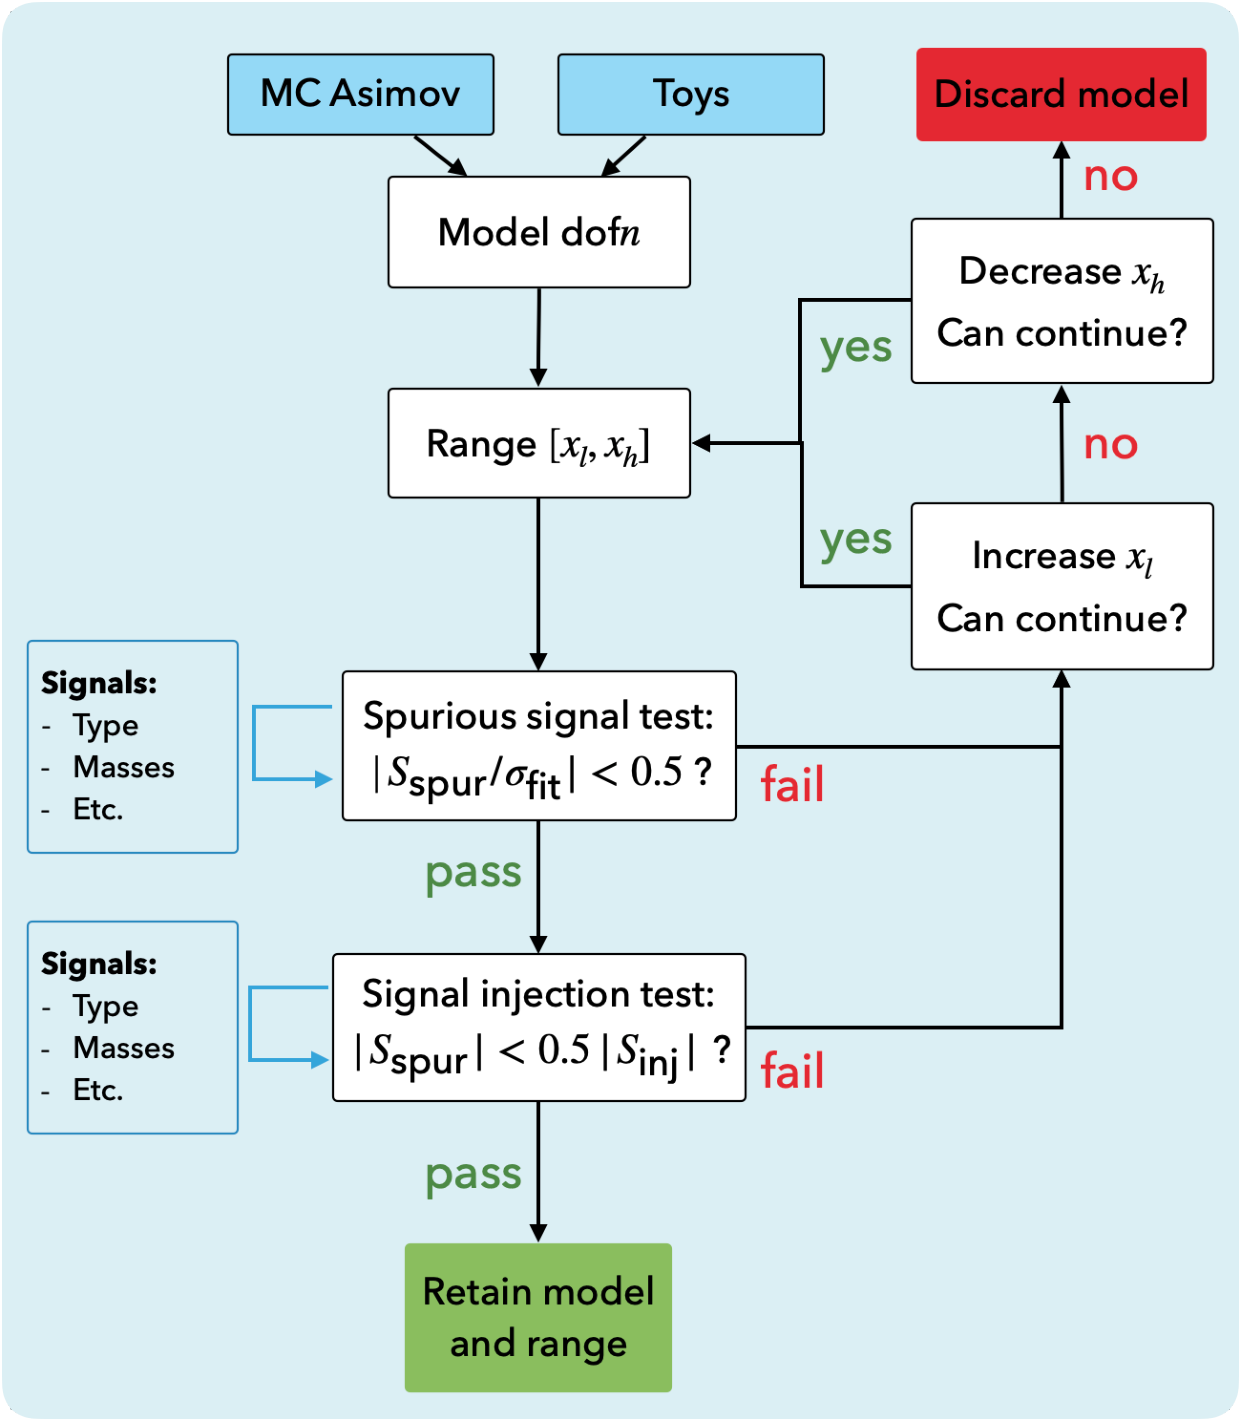
\includegraphics[width=0.5\textwidth]{5_resonances/bkg/modeling/fitmodel_validation}
    \caption{Flowchart for the fit function and fit-range validation done using \ac{MC} samples.}
    \label{fig:bkg:modeling:strategy:fitmodel_validation}
\end{figure}

The process to select an optimal fit-range and functional model combination is schematised in \Fig{\ref{fig:bkg:modeling:strategy:fitmodel_validation}}.
The validation process is carried out with \ac{MC}, for both, toys and Asimov datasets. As a first step, \ac{BO} fits to the Asimov dataset need to pass the requirements shown in \Fig{\ref{fig:bkg:modeling:preparation:datasets_generation}} (\(p(\chisq) > 0.05\)) and then toys sets are computed. The first test to which the datasets are subjected to is the \acf{SSig} test. Those models and ranges passing this particular test are then the input to \ac{SI} tests. In case all these pass, the fit function is retained and will be subjected to another test, discussed below. There are cases in which the functional models do not pass these requiremenets. To treat those cases, the first step is to increase the lower limit of the fit, and the whole procedure is carried out again. When the lower limit cannot be increased anymore, the higher limit can be decreased, taking into account that all the signal models need to be acommodated. For each one of the tests said above, a complete explanation with results is presented in the following sections.

% Using a small portion of the complete dataset, all the selected functions are evaluated again, in a similar way as it is done for MC (see \Fig{\ref{fig:bkg_modeling:fitmodel_validation_data}}). The only modification to the above procedure is that a window-exclusion fit is performed using BumpHunter in case the first fit to data fails.


With the selected functions and fit ranges, the function choice is performed based on \(F\)-test, and a ranking of the fit models and ranges is created based on the \(\sigma_{\text{fit}}\) obtained from \ac{SSig} tests, schematized in \Fig{\ref{fig:bkg:modeling:strategy:fitmodel_selection}}

\begin{figure}[ht!]
    \centering
    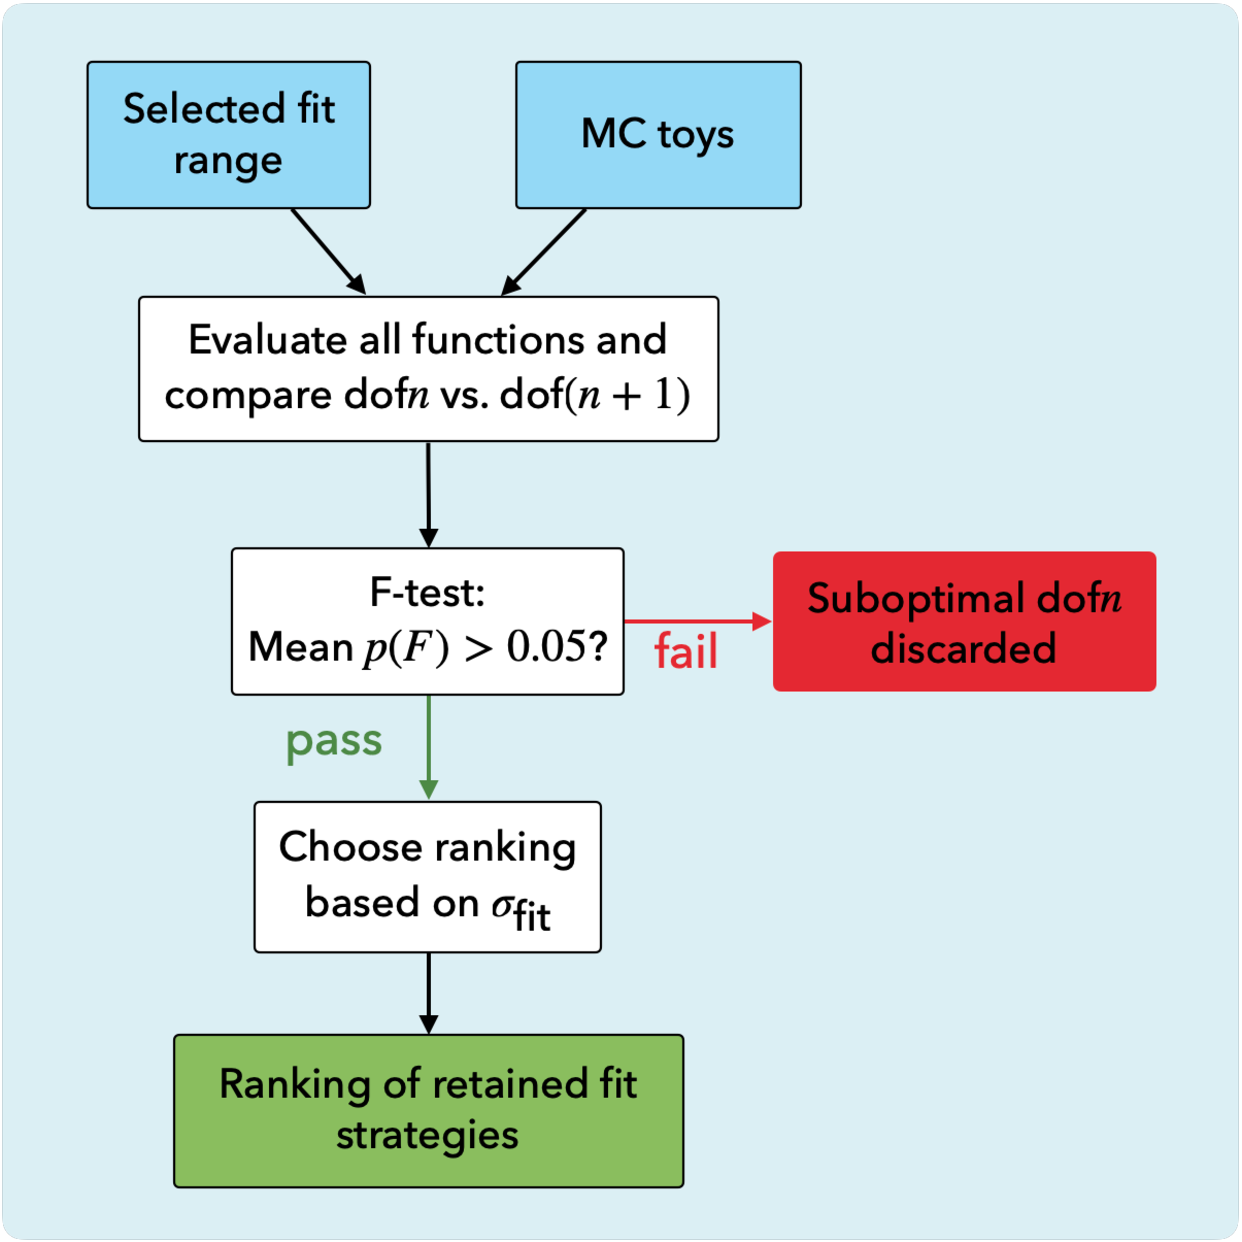
\includegraphics[width=0.5\textwidth]{5_resonances/bkg/modeling/unblind_strategy2}
    \caption{Scheme of the fit function selection based on the \(F\)-test.}
    \label{fig:bkg:modeling:strategy:fitmodel_selection}
\end{figure}




%%%%%%%%%%%%%%%%%%%%%%%%%%%%%%%%%%%%%%%%%%%%%%%%%%%%%%%%%%%%%%%%%%%%%%%%%%%%%%%%%%%%%%%%%%%%%%%%%%%%
%%%%%%%%%%%%%%%%%%%%%%%%%%%%%%%%%%%%%%%%%%%%%%%%%%%%%%%%%%%%%%%%%%%%%%%%%%%%%%%%%%%%%%%%%%%%%%%%%%%%
%%%%%%%%%%%%%%%%%%%%%%%%%%%%%%%%%%%%%%%%%%%%%%%%%%%%%%%%%%%%%%%%%%%%%%%%%%%%%%%%%%%%%%%%%%%%%%%%%%%%





























%%%%%%%%%%%%%%%%%%%%%%%%%%%%%%%%%%%%%%%%%%%%%%%%%%%%%%%%%%%%%%%%%%%%%%%%%%%%%%%%%%%%%%%%%%%%%%%%%%%%
%%%%%%%%%%%%%%%%%%%%%%%%%%%%%%%%%%%%%%%%%%%%%%%%%%%%%%%%%%%%%%%%%%%%%%%%%%%%%%%%%%%%%%%%%%%%%%%%%%%%
%%%%%%%%%%%%%%%%%%%%%%%%%%%%%%%%%%%%%%%%%%%%%%%%%%%%%%%%%%%%%%%%%%%%%%%%%%%%%%%%%%%%%%%%%%%%%%%%%%%%
\subsection{Fit strategy validation}
\label{subsec:bkg:modeling:sigbkg}

In the following sections, a detailed discussion of each part of the modeling strategy for the background is presented. As shown in \Fig{\ref{fig:bkg:modeling:strategy:fitmodel_validation}}, the process starts by computing \ac{SSig} and \ac{SI} tests, in oder to first gather the possible functions and fit-ranges to use in the final fits to data. These fit-range/fit-function combination pairs are then ranked based on the \ac{SSig} value. Finally, the \(F\)-test is used to reorder these combinations.

%%%%%%%%%%%%%%%%%%%%%%%%%%%%%%%%%%%%%%%%%%%%%%%%%%%%%%%%%%%%%%%%%%%%%%%%%%%%%%%%%%%%%%%%%%%%%%%%%%%%
\subsubsection{Spurious signal tests}
\label{subsubsec:bkg:modeling:sigbkg:sstest}

The fit bias, or \acf{SSig}, is estimated by fitting a \ac{BO} distribution with a \ac{SB} composite model, in which one of the components is the signal template obtained from the interpolated signals (or a gaussian), and the background component being the different functional models evaluated throughout this section.
The \ac{SSig} (\sspur) and its uncertainty (\(\sigma_{\text{fit}}\)) are obtained from the resulting signal yield (\(N_{\text{sig}}\)) after the fit to the \ac{BO} distribution. In an ideal case, \sspur should approximate to zero, indicating that the functional model selected for the background correctly captures the whole distribution.
The \ac{SSig} can also be computed from fits to the toys distributions. In such cases, \sspur is the mean value of all the experiments carried out, and \(\sigma_{\text{fit}}\) is computed as the RMS of the \sspur distribution. The two definitions of the \ac{SS} value therefore are:
\begin{equation}
    \label{eq:bkg:modeling:sigbkg:sstest:sspur_definition_sstest}
    \sspur = 
    \begin{cases}
        N_{\text{sig}} & \qif \text{Asimov dataset},\\
        \expval{N_{\text{sig}}}_{\text{toys}} & \qif \text{Toys dataset}.
    \end{cases}
\end{equation}

The calculation is done for each one of the signal masses for each model, at each one of the signal regions. The \ac{BO} distribution can either be the asimov dataset or the whole set of toys distributions. In \Fig{\ref{fig:bkg:modeling:sigbkg:sstest:sstest_asimov_examples}}, two examples of fits to the asimov dataset is shown for the inclusive region, SR. The signal models taken into account are both \qstar with \(f=1.0\) and using masses \(\mq = 2000~\gev\) and \(\mq = 6000~\gev\). The functional model used to model the background is the \textit{dof2} model and the fit is done in the \myj range of \(800-10000~\gev\).

\begin{figure}[ht!]
    \centering
    \begin{subfigure}[h]{0.49\linewidth}
        \centering
        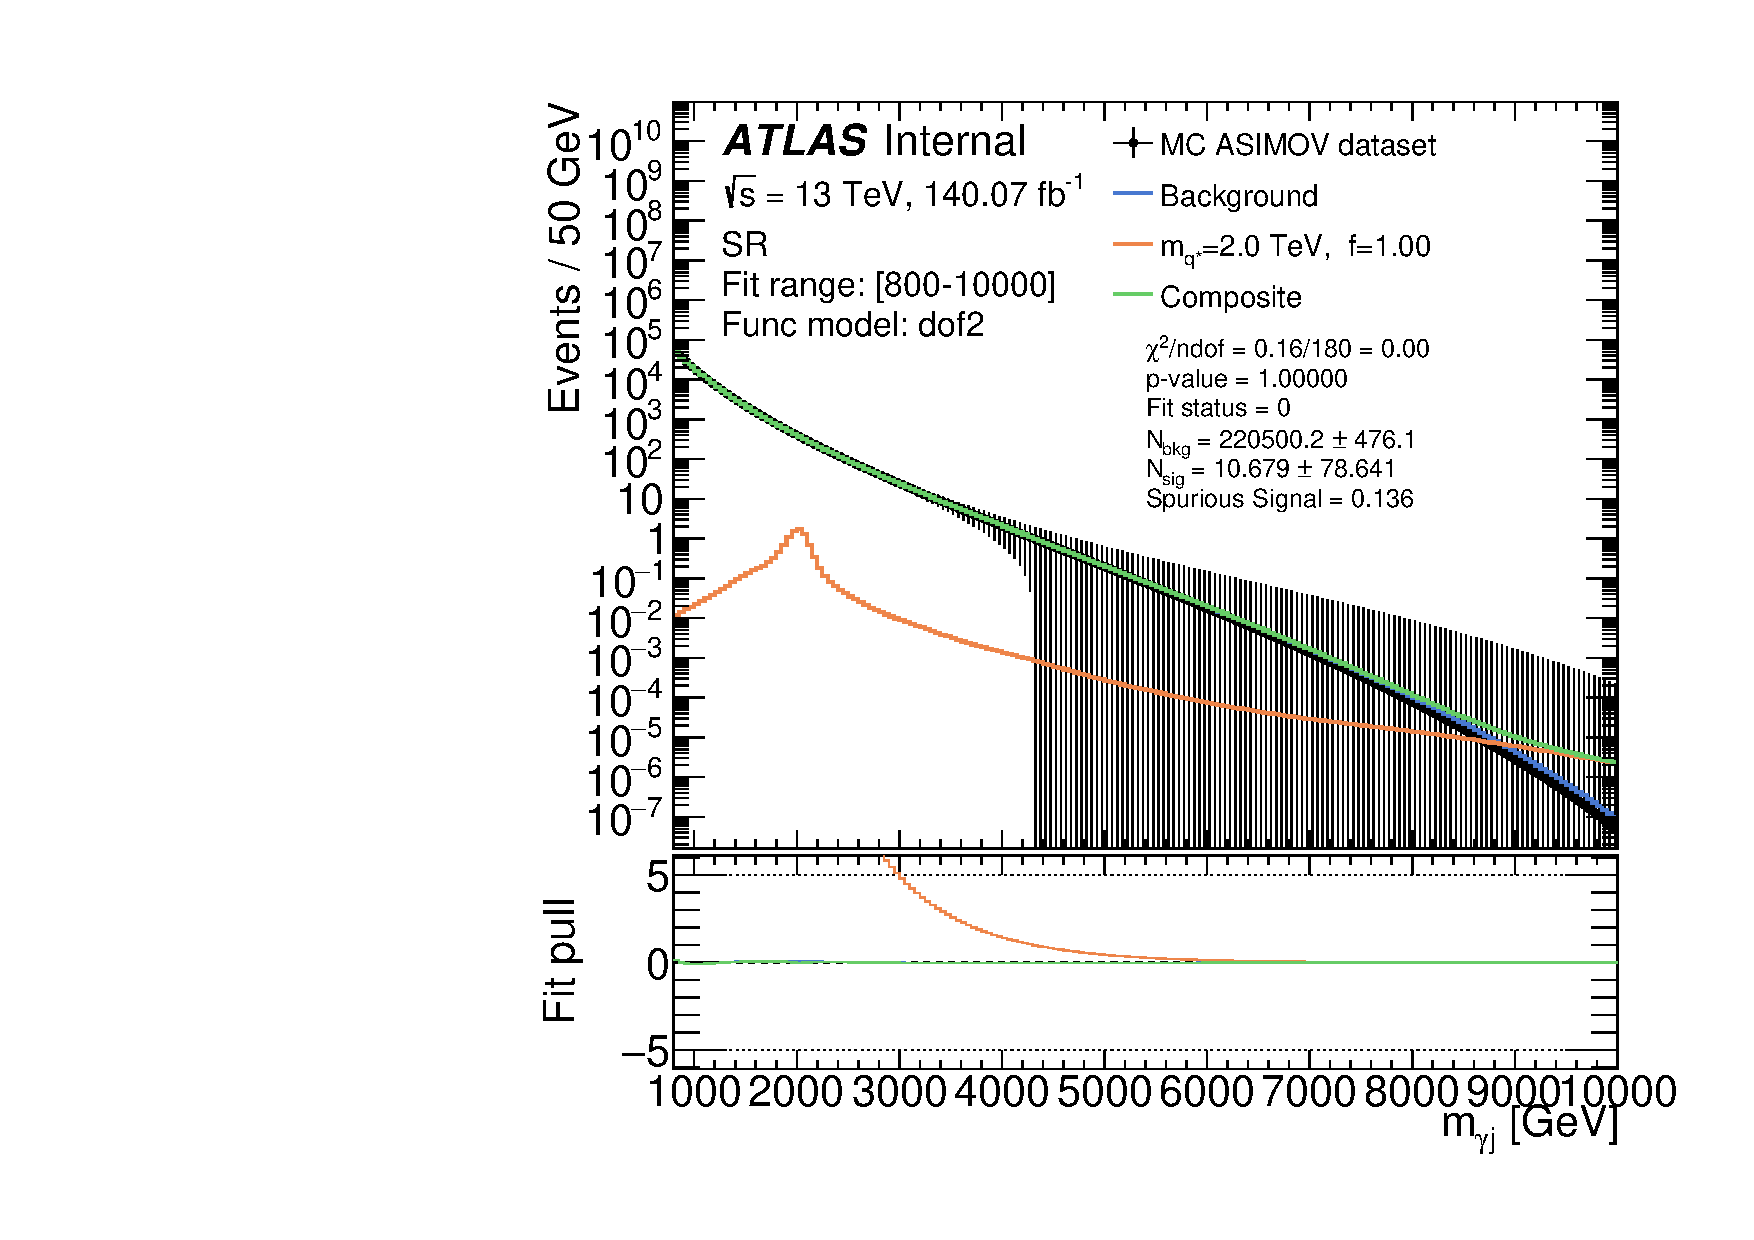
\includegraphics[width=\textwidth]{5_resonances/bkg/modeling/ss/asimov/fits/can__sigbkg_fit__asimov__photonjet_Pythia__SR__dof2__range_800-10000__qstar__qStar_f1p00_M2000}
        \caption{\(m_{\qstar} = 2000~\gev\)}
    \end{subfigure}
    \hfill
    \begin{subfigure}[h]{0.49\linewidth}
        \centering
        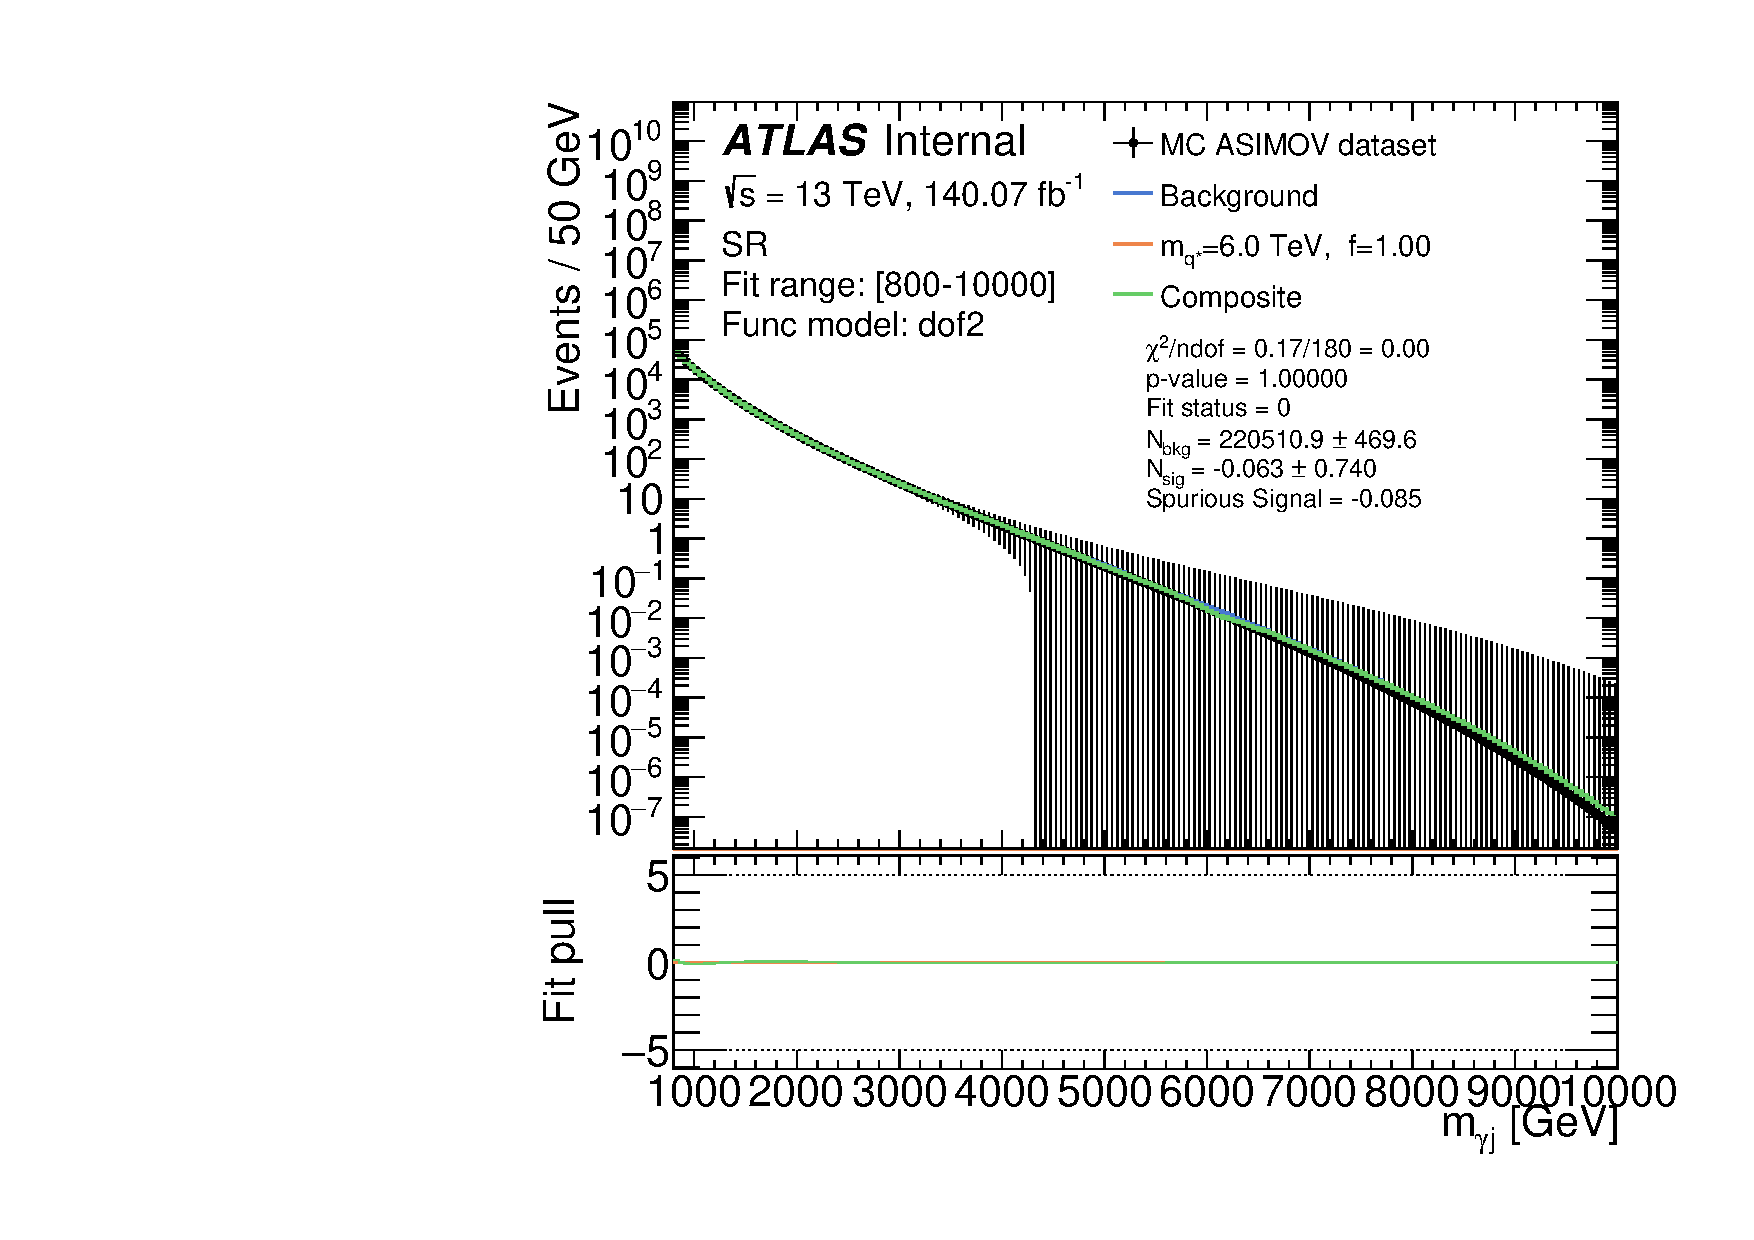
\includegraphics[width=\textwidth]{5_resonances/bkg/modeling/ss/asimov/fits/can__sigbkg_fit__asimov__photonjet_Pythia__SR__dof2__range_800-10000__qstar__qStar_f1p00_M6000}
        \caption{\(m_{\qstar} = 6000~\gev\)}
    \end{subfigure}
    \caption{\ac{SB} fit to the Asimov background distribution for the calculation of \ac{SSig}. The signal model, with floating normalization, is shown with the orange line, the functional model in this case the \textit{dof2}, represented by the blue line, and the composite fit is shown in green. The figure on the right shows a case in which the \ac{SSig} is negative.}
    \label{fig:bkg:modeling:sigbkg:sstest:sstest_asimov_examples}
\end{figure}

\begin{figure}[ht!]
    \centering
    \begin{subfigure}[h]{0.49\linewidth}
        \centering
        \includegraphics[width=\textwidth, page=24]{5_resonances/bkg/modeling/ss/toys/fits/can__sigbkg_fit__toys__photonjet_Pythia__SR__dof2__range_800-10000__qstar__qStar_f1p00_M2000}
    \end{subfigure}
    \hfill
    \begin{subfigure}[h]{0.49\linewidth}
        \centering
        \includegraphics[width=\textwidth, page=423]{5_resonances/bkg/modeling/ss/toys/fits/can__sigbkg_fit__toys__photonjet_Pythia__SR__dof2__range_800-10000__qstar__qStar_f1p00_M2000}
    \end{subfigure}
    \caption{Same as \Fig{\ref{fig:bkg:modeling:sigbkg:sstest:sstest_asimov_examples}} but using background toys distributions}
    \label{fig:bkg:modeling:sigbkg:sstest:sstest_toys_examples}
\end{figure}

Fit to toys, on the other hand, are shown in \Fig{\ref{fig:bkg:modeling:sigbkg:sstest:sstest_toys_examples}}, in the same conditions as shown in \Fig{\ref{fig:bkg:modeling:sigbkg:sstest:sstest_asimov_examples}}, only for the \(m_{\qstar}=2000~\gev\) model. As mentioned above, the final result of \ac{SSig} for the toys is obtained from the \sspur distribution of all the fits that are successful. As an example, fits to the inclusive SR using \qstar signals in the range \(800-10000~\gev\) and with the function \textit{dof2} are shown in \Fig{\ref{fig:bkg_modeling:sstest_toys_distributions}}. From the figures, two different \qstar masses are shown: \(2000\) and \(4000~\gev\). In the first case, the mean value of the \sspur is much higher than in the second case, but with higher standard deviation as well.
\begin{figure}[ht!]
    \centering
    \begin{subfigure}[h]{0.49\linewidth}
        \centering
        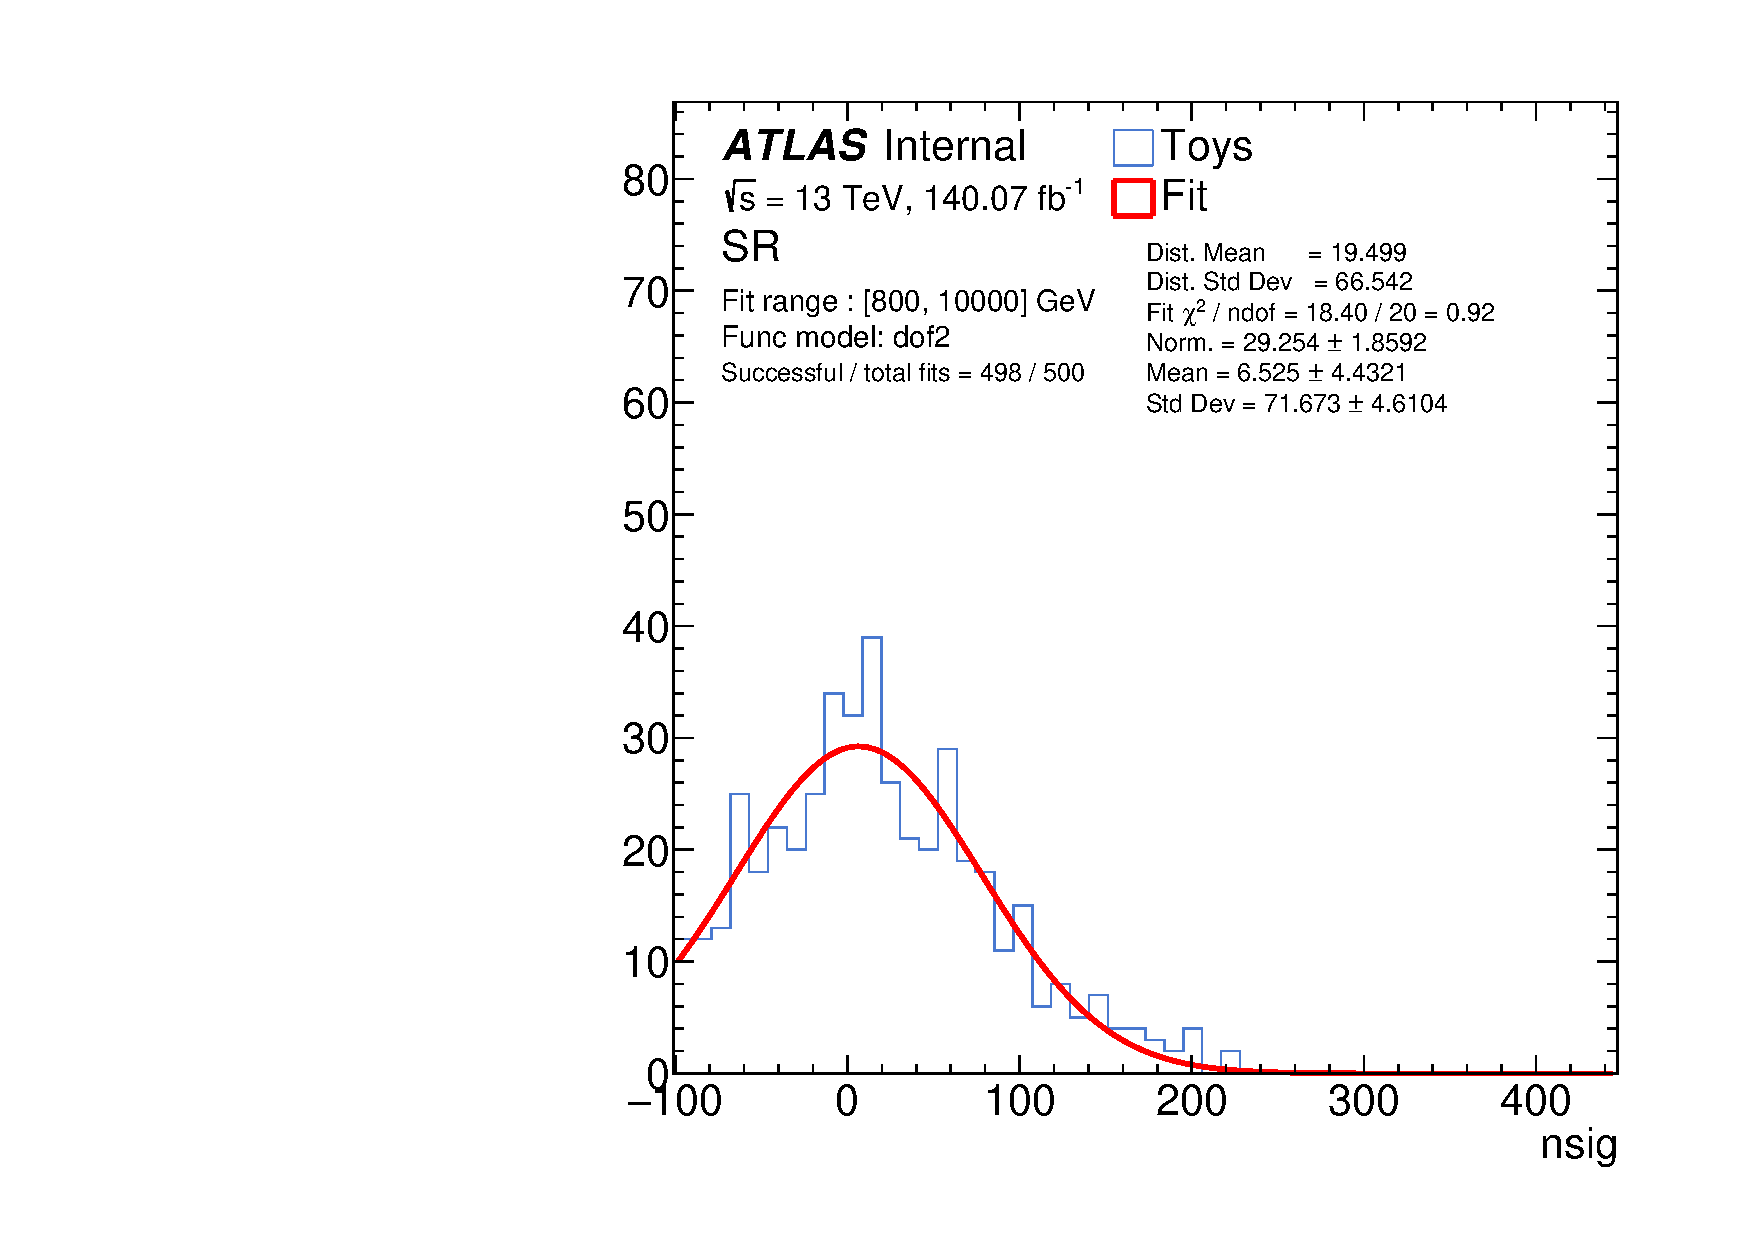
\includegraphics[width=\textwidth]{5_resonances/bkg/modeling/ss/toys/fits/can__photonjet_Pythia__SR__dof2__range_800_10000__qStar_f1p00_M2000__toys_nsig}
        \caption{\(\mq = 2000~\gev\)}
    \end{subfigure}
    \hfill
    \begin{subfigure}[h]{0.49\linewidth}
        \centering
        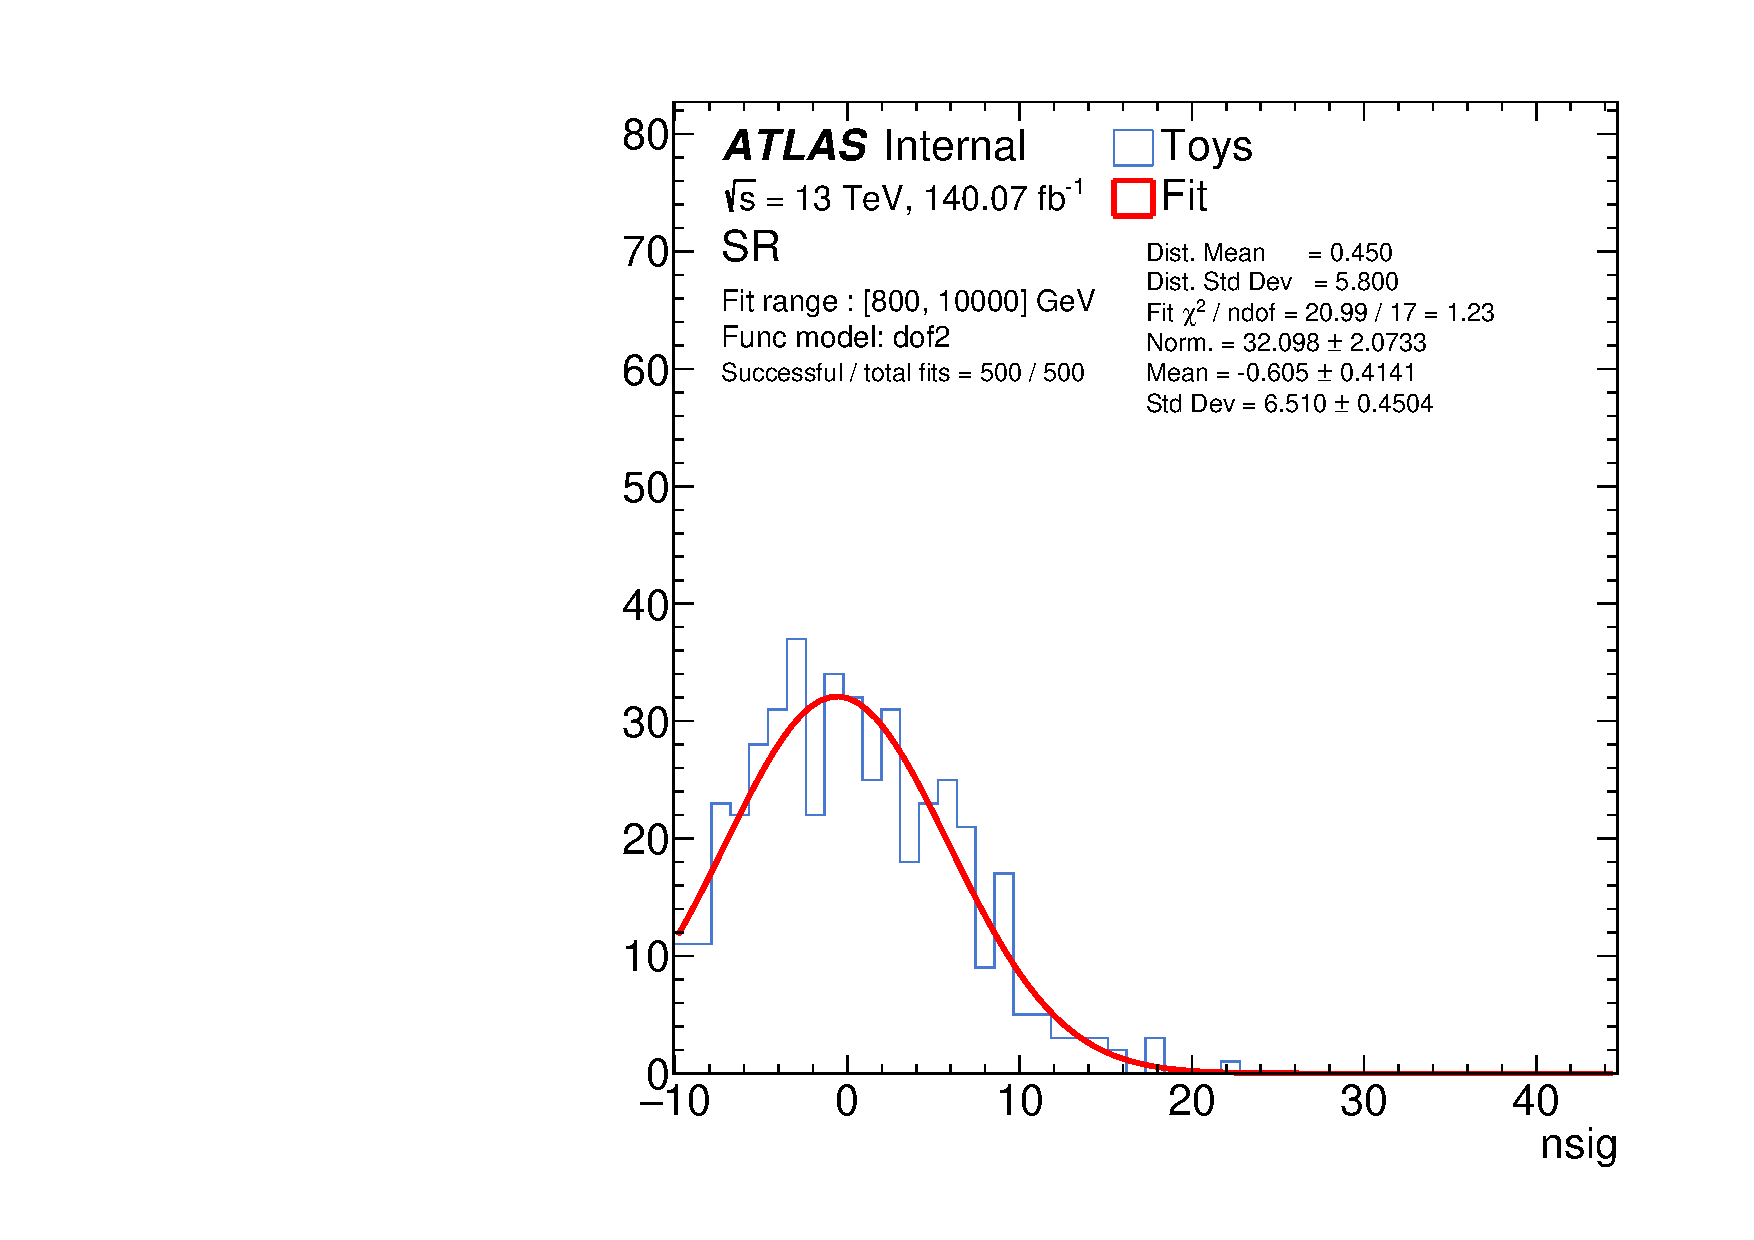
\includegraphics[width=\textwidth]{5_resonances/bkg/modeling/ss/toys/fits/can__photonjet_Pythia__SR__dof2__range_800_10000__qStar_f1p00_M4000__toys_nsig}
        \caption{\(\mq = 4000~\gev\)}
    \end{subfigure}
    \caption{\sspur distribution (blue line) in the SR region, with a gaussian fit to it. The final \sspur value is directly taken from the distribution, not from the fit. The functional model is \textit{dof2} and the background is fitted within the range \([800, 1000]~\gev\). The \ac{EQ} signal model is used contemplating only \qstar with cupling \(f=1.0\).}
    \label{fig:bkg_modeling:sstest_toys_distributions}
\end{figure}


In general, for a model to pass the test, the \sspur needs to be within the acceptable bounds of:
\begin{equation*}
    |\sspur| < 0.5 \sigma_{\text{fit}}
\end{equation*}
and after that they can be used for further studies. In both cases shown in \Fig{\ref{fig:bkg_modeling:sstest_toys_distributions}}, the \ac{SSig} test is passed, where the \(\sspur / \sigma_{\text{fit}}\) ratios are \(19.5 / 66.5 = 0.29\) and \(0.45 / 5.80 = 0.07\) for the \(\mq = 2000\) and \(\mq = 4000~\gev\) masses, respectively.
The main purpose of these tests is to find a group of appropriate functions to be used, as well as the optimal fit range for these functional models. Different lower and upper bounds for the fit ranges are considered depending on the signal region being studied.


\Fig{\ref{fig:bkg_modeling:sstest_results_asimov_SR}} shows the \ac{SSig} for the different considered signal models in the inclusive region SR. The selected results correspond to using the \ac{MC} asimov dataset and the fit-range is the one that yields the lowest \ac{SSig}. Each figure shows different functional models (different \ac{dof}). Similarly, \ac{SSig} results from toys datasets are shown in \Fig{\ref{fig:bkg_modeling:sstest_results_toys_SR}}.

It can be noted from the comparison of \Fig{\ref{fig:bkg_modeling:sstest_results_asimov_SR}} (asimov) and \Fig{\ref{fig:bkg_modeling:sstest_results_toys_SR}} (toys), that for toys, the \ac{SSig} tests have been carried out for signals with masses up to \(5000~\gev\). The reason behind this is the absence of events in the \myj distributions for \(\myj \gtrsim 5.5~\tev\), therefore a \ac{SB} fit to zero events lacks of phyisical meaning. A discussion on the maximum \myj distribution was presented in \Sect{\ref{subsubsec:bkg:modeling:preparation:toys}}, where the maximum \myj value for each signal region was shown.


\begin{figure}[ht!]
    \centering
    \begin{subfigure}[h]{0.32\linewidth}
        \centering
        \includegraphics[width=\textwidth]{5_resonances/bkg/modeling/ss/asimov/results/SR/gaus/width0p02/plots/can__SS__photonjet_Pythia__gaus__SR__width0p02__range_1200_8000}
        \caption{Gaussian with \(\sigma_G / \mG = 0.02\).}
    \end{subfigure}
    \hfill
    \begin{subfigure}[h]{0.32\linewidth}
        \centering
        \includegraphics[width=\textwidth]{5_resonances/bkg/modeling/ss/asimov/results/SR/qstar/q_1p00/plots/can__SS__photonjet_Pythia__qstar__SR__q_1p00__range_1000_8000}
        \caption{\qstar.}
    \end{subfigure}
    \begin{subfigure}[h]{0.32\linewidth}
        \centering
        \includegraphics[width=\textwidth]{5_resonances/bkg/modeling/ss/asimov/results/SR/QBH/n1/plots/can__SS__photonjet_Pythia__QBH__SR__n1__range_1000_8000}
        \caption{\ac{QBH} with \(n=1\).}
    \end{subfigure}\\
    \caption{\ac{SSig} tests results for the inclusive SR region. The different figures correspond to the fit-range that yields the lowest \ac{SSig} for the given signal model and function's \ac{dof}. Different functional forms are shown with different colors.}
    \label{fig:bkg_modeling:sstest_results_asimov_SR}
\end{figure}


\begin{figure}[ht!]
    \centering
    \begin{subfigure}[h]{0.32\linewidth}
        \centering
        \includegraphics[width=\textwidth]{5_resonances/bkg/modeling/ss/toys/results/SR/gaus/width0p02/plots/can__SS__photonjet_Pythia__gaus__SR__width0p02__range_1200_8000}
        \caption{Gaussian with \(\sigma_G / \mG = 0.02\).}
    \end{subfigure}
    \hfill
    \begin{subfigure}[h]{0.32\linewidth}
        \centering
        \includegraphics[width=\textwidth]{5_resonances/bkg/modeling/ss/toys/results/SR/qstar/q_1p00/plots/can__SS__photonjet_Pythia__qstar__SR__q_1p00__range_1000_8000}
        \caption{\qstar.}
    \end{subfigure}
    \begin{subfigure}[h]{0.32\linewidth}
        \centering
        \includegraphics[width=\textwidth]{5_resonances/bkg/modeling/ss/toys/results/SR/QBH/n1/plots/can__SS__photonjet_Pythia__QBH__SR__n1__range_1000_8000}
        \caption{\ac{QBH} with \(n=1\).}
    \end{subfigure}\\
    \caption{Idem \Fig{\ref{fig:bkg_modeling:sstest_results_asimov_SR}} but using toy samples.}
    \label{fig:bkg_modeling:sstest_results_toys_SR}
\end{figure}


Due to the two methodologies (toys and asimov datasets) used to compute the \ac{SSig} test, results from both calculations are combined giving preference to toys, as they are calculated in a more robust form. The combination is performed as follows:
\begin{enumerate}
    \item Use toys \ac{SSig} results up to the mass point where it is expected to have a considerable amount of background events. The maximum mass point considered for all those regions that are dominated by \ljets (\bjets and \cjets) is \(<5~\tev\) (\(<4~\tev\)). Toy \ac{SSig} results therefore only contribute on the low mass regime.
    \item Asimov \ac{SSig} results are used for the rest of the mass range, hence contributing only to the high mass region of the spectrum.
\end{enumerate}
The \ac{SSig}, or fit bias, is used in the final limit calculation as one of the systematic uncertainties associated with the background modeling, therefore it is then desired that this uncertainty is as small as possible. For each signal region and signal model, after the previously mentioned combination is performed, a ranking of the fit-ranges and functional models is created, based on the average absolute \ac{SSig}. This quantity indicates which combination of fit-range and functional model provides the lowest \ac{SSig} in average for each mass point, giving equal importance to each mass.
% Examples of these rankings are presented in \Tab{\ref{tab:bkg_modeling:ss_test:ss_ranking_SR}}.


% \begin{table}[ht!]
%     \centering
%     \caption{Fit-range and functional model combination giving the lowest \ac{SSig} for the three different signal models considered in the SR.}
%     \begin{minipage}{0.45\textwidth}
%         \centering
%         \subcaption{\qstar}
%         \includegraphics[width=\textwidth]{example-image}
%         % \input{figures/background_modeling/spurious_signal/tables/sig__qstar__SS_rank__SR__qStar.tex}
%     \end{minipage}\hfill
%     \begin{minipage}{0.45\textwidth}
%         \centering
%         \subcaption{\qbh}
%         \includegraphics[width=\textwidth]{example-image}
%         % \input{figures/background_modeling/spurious_signal/tables/sig__QBH__SS_rank__SR__total.tex}
%     \end{minipage}\\
%     \vspace{1.2em}
%     \begin{minipage}{0.45\textwidth}
%         \centering
%         \subcaption{Gaussians}
%         \includegraphics[width=\textwidth]{example-image}
%         % \input{figures/background_modeling/spurious_signal/tables/sig__gaus__SS_rank__SR__total.tex}
%     \end{minipage}\\
%     \label{tab:bkg_modeling:ss_test:ss_ranking_SR}
% \end{table}
%%%%%%%%%%%%%%%%%%%%%%%%%%%%%%%%%%%%%%%%%%%%%%%%%%%%%%%%%%%%%%%%%%%%%%%%%%%%%%%%%%%%%%%%%%%%%%%%%%%%




%%%%%%%%%%%%%%%%%%%%%%%%%%%%%%%%%%%%%%%%%%%%%%%%%%%%%%%%%%%%%%%%%%%%%%%%%%%%%%%%%%%%%%%%%%%%%%%%%%%%
\subsubsection{Signal injection tests}
\label{subsubsec:bkg:modeling:sigbkg:sitest}

A \acf{SI} test probes the ability of a fit strategy to correctly determine the amount of signal present in a dataset. It is performed similarly to the \ac{SSig} test, with the difference that a signal of the expected hypothesis is injected with a certain amplitude on top of the \ac{BO} pseudo-data or toys. While the definition of \sspur for the \ac{SSig} tests was simply the number of extracted signal events, shown by \Eqn{\ref{eq:bkg:modeling:sigbkg:sstest:sspur_definition_sstest}}, in these tests it is generalised such that \sspur is now the difference between the extracted and the injected signals:
\begin{equation}
    \label{eq:bkg:modeling:sigbkg:sitest:sspur_definition}
    \sspur = 
    \begin{cases}
        N_{\text{fit}} - N_{\text{inj}} & \qif \text{Asimov dataset},\\
        \expval{N_{\text{fit}} - N_{\text{inj}}}_{\text{toys}} & \qif \text{Toys dataset}.
    \end{cases}
\end{equation}

The amplitude of the injection is denoted in units of \(\sqrt{B}\), which takes into account the square root of the number of background events in the \ac{FWHM} range of the signal in question, corrected by the number of signal events in the range:
\begin{equation*}
    \sqrt{B} \equiv \frac{
        \displaystyle
        \sqrt{\sum_{\text{bins in FWHM}} b_i}
        }{
        \displaystyle
        \sum_{\text{bins in FWHM}} s_i 
    }
\end{equation*}
The inclusion of this correction aims to have the reported amplitudes in units of \(\sqrt{B}\) to always correspond to \(S / \sqrt{B}\) ratios. 

To evaluate the \ac{SI} tests, 300 toy experiments are run per signal hypothesis, per signal region and injection amplitude, in the same ranges as in the \ac{SSig} tests, and using different functional models. The recommended criterion for passing the signal injection tests is \(|\sspur| < 0.5 N_{\text{inj}}\). In \Fig{\ref{fig:bkg:modeling:sigbkg:sitest:siginj_qstar}}, examples of the test for the \ac{EQ} signal model are shown. The upper pad of the figures show, as a function of \(N_{\text{sig}}^{\text{inj}} / \sqrt{B}\), the extracted signal in the \ac{FWHM} range \(N_{\text{sig}}^{\text{fit}} / \sqrt{B}\) for different masses. The bottom pad of the plots show the \sspur calculated as in \Eqn{\ref{eq:bkg:modeling:sigbkg:sitest:sspur_definition}}, divided by the injected signal amplitude \(N_{\text{inj}}\). In all cases, the \ac{SI} test is passed as the ratio is \(<0.5\). Moreover, it can be seen that the results show very good linearity. Results for the other signal models are shown in \App{\ref{app:si_results}} where good linearity is seen for all cases.
\fixme{revise definition of ratio. Should it be with the uncertainty, or with the injecected signal?}

\begin{figure}[ht!]
    \centering
    \begin{subfigure}[h]{0.49\linewidth}
        \centering
        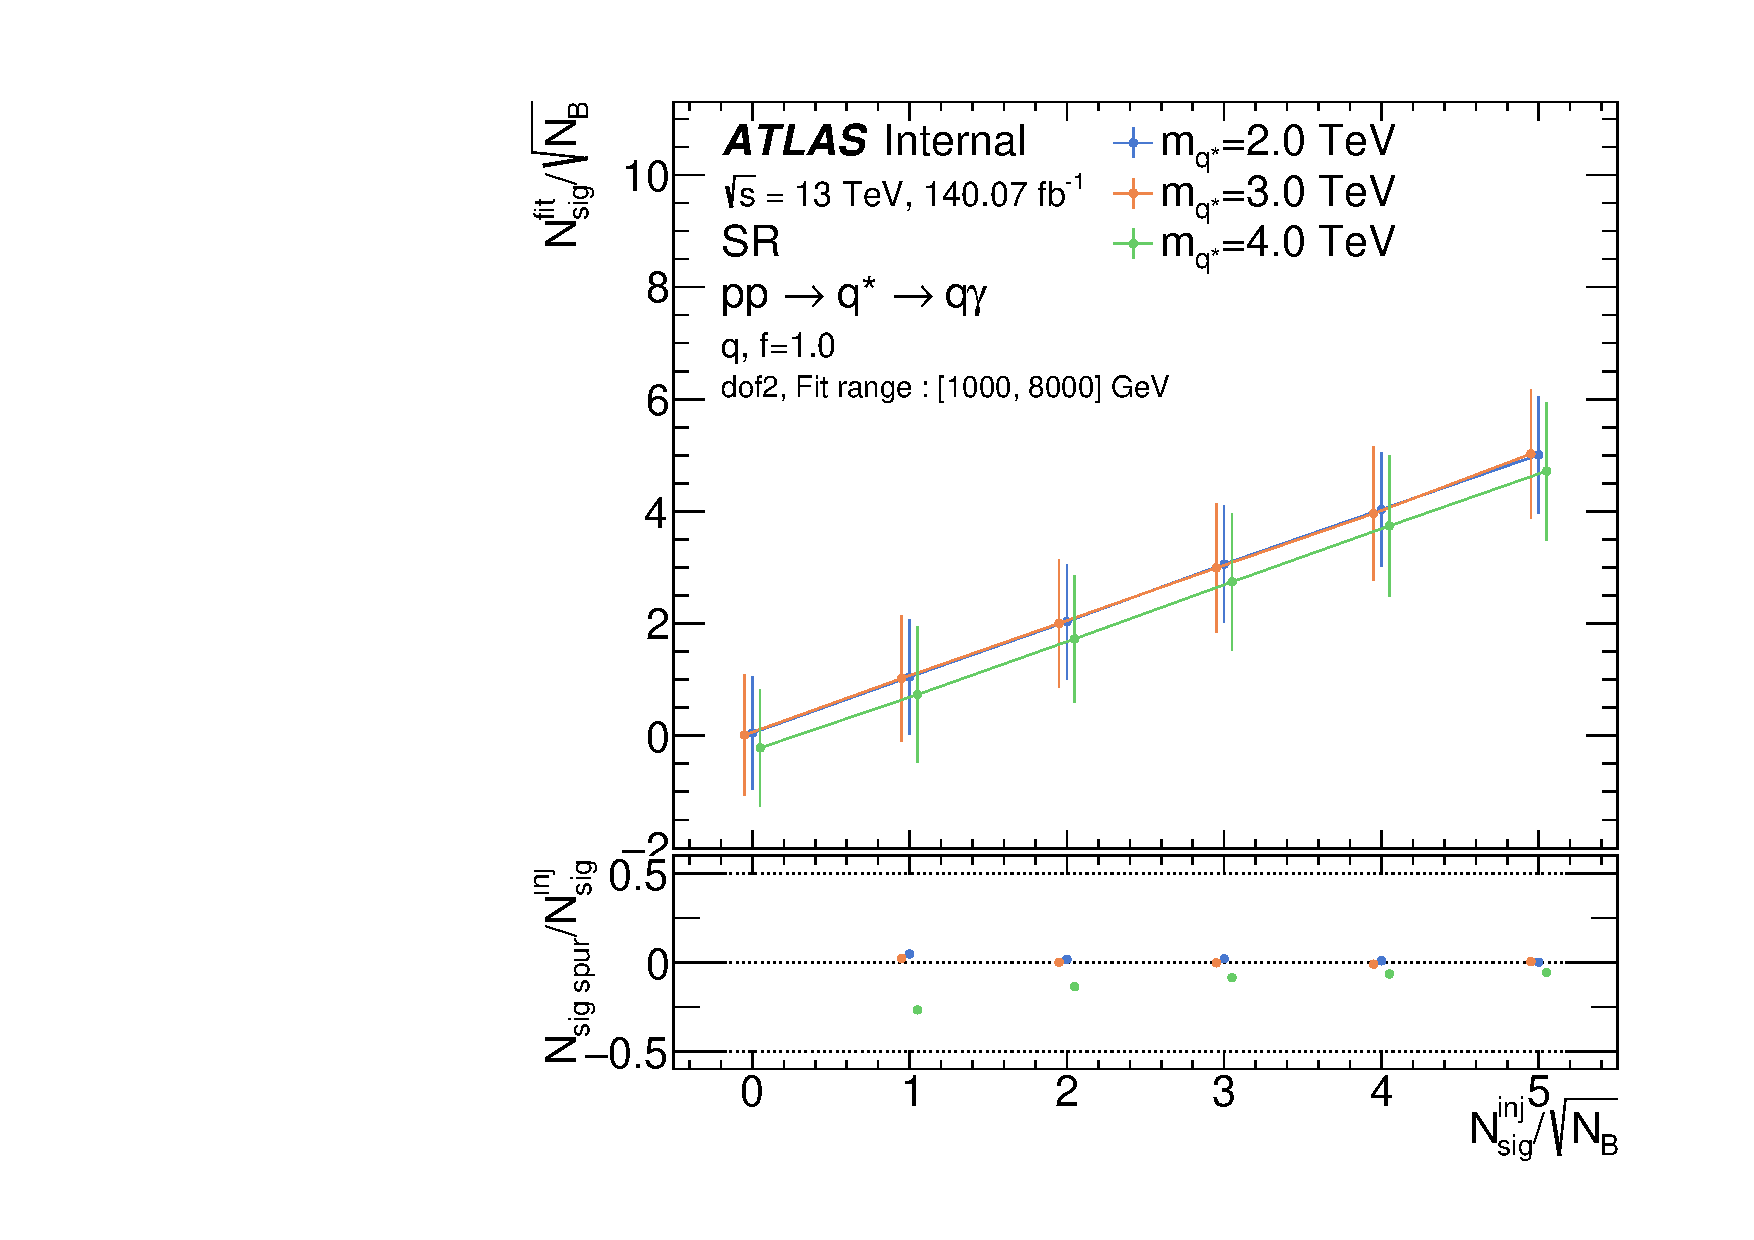
\includegraphics[width=\textwidth]{5_resonances/bkg/modeling/si/toys/SR/qstar/q_1p00/dof2__range_1000_8000/plots/can__SigInj__photonjet_Pythia_jfakeisosmooth__qstar__SR__q_1p00__dof2__range_1000_8000}
        \caption{SR.}
    \end{subfigure}
    \hfill
    \begin{subfigure}[h]{0.49\linewidth}
        \centering
        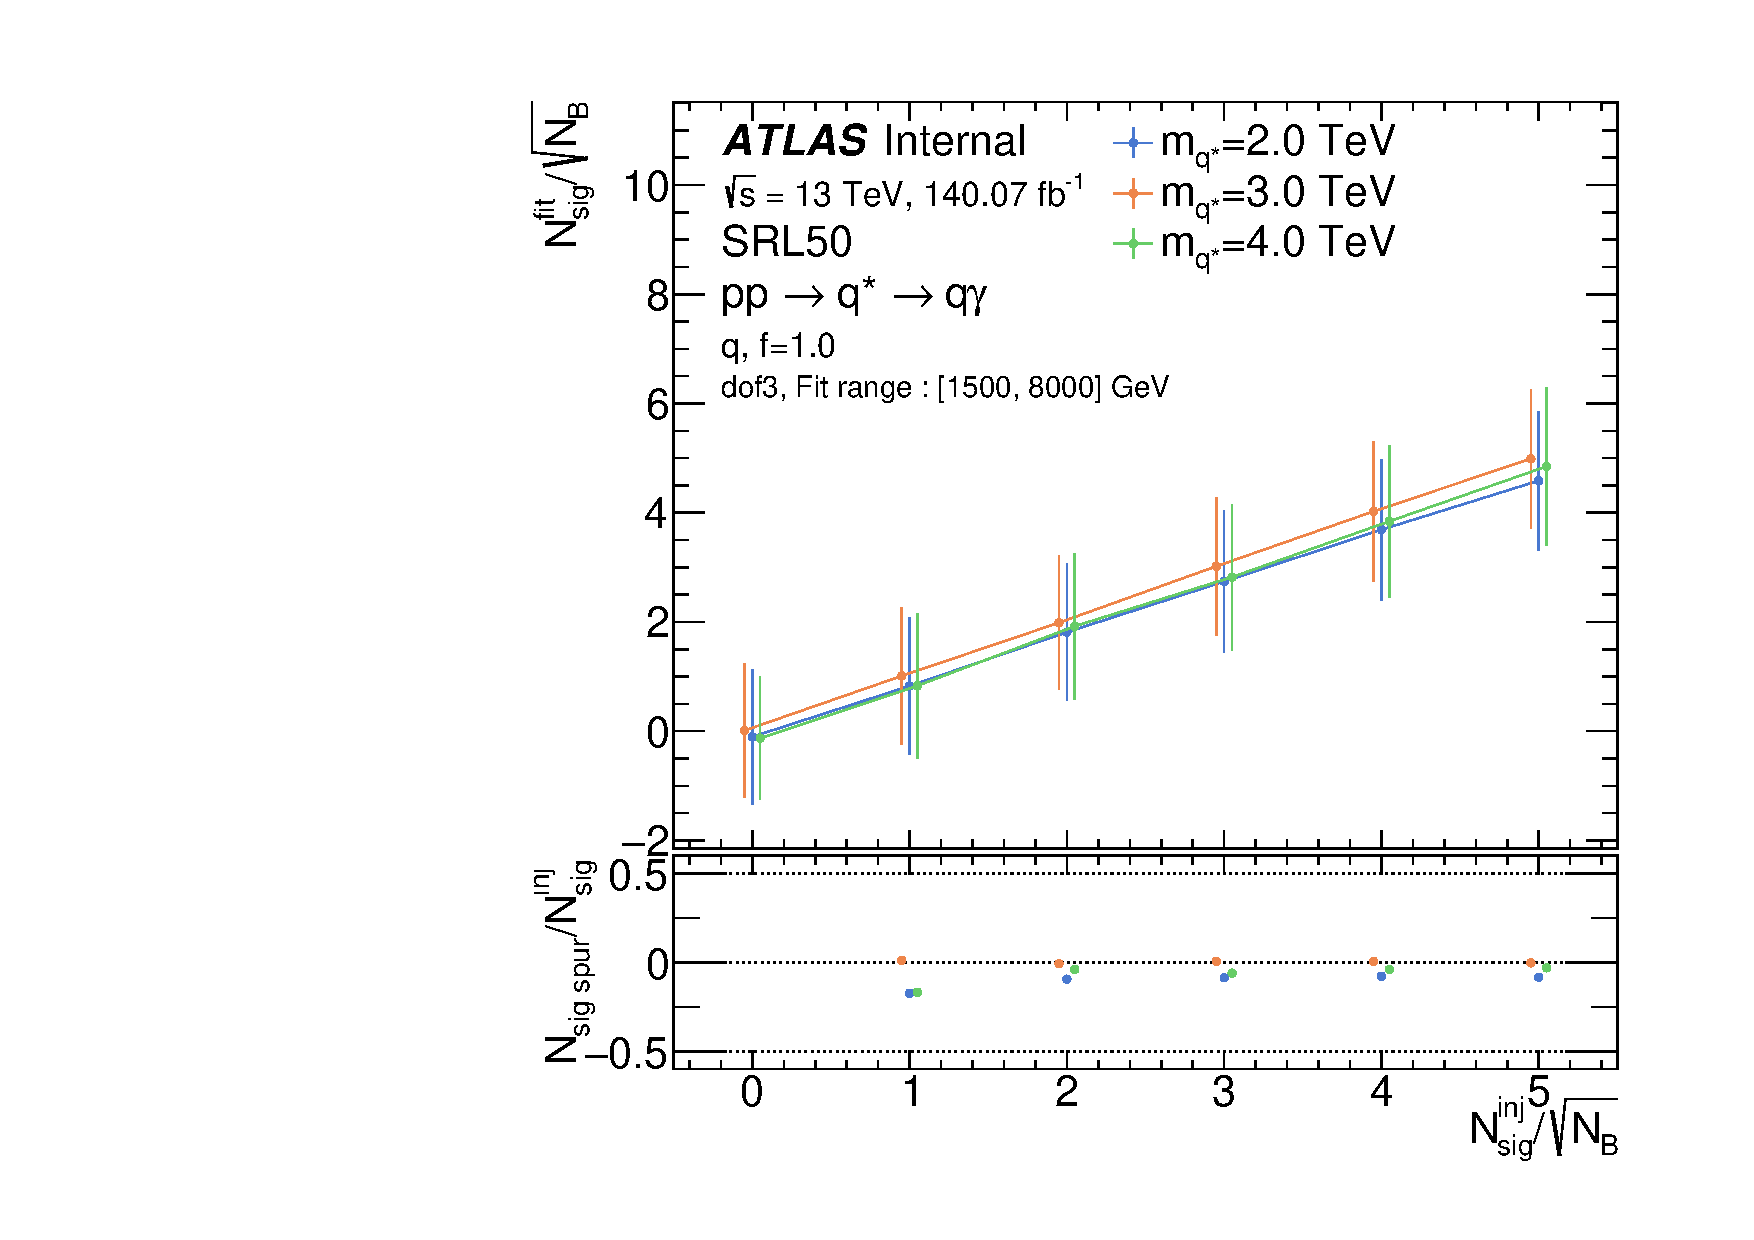
\includegraphics[width=\textwidth]{5_resonances/bkg/modeling/si/toys/SRL50/qstar/q_1p00/dof3__range_1500_8000/plots/can__SigInj__photonjet_Pythia_jfakeisosmooth__qstar__SRL50__q_1p00__dof3__range_1500_8000}
        \caption{SRL.}
    \end{subfigure}\\
    \begin{subfigure}[h]{0.49\linewidth}
        \centering
        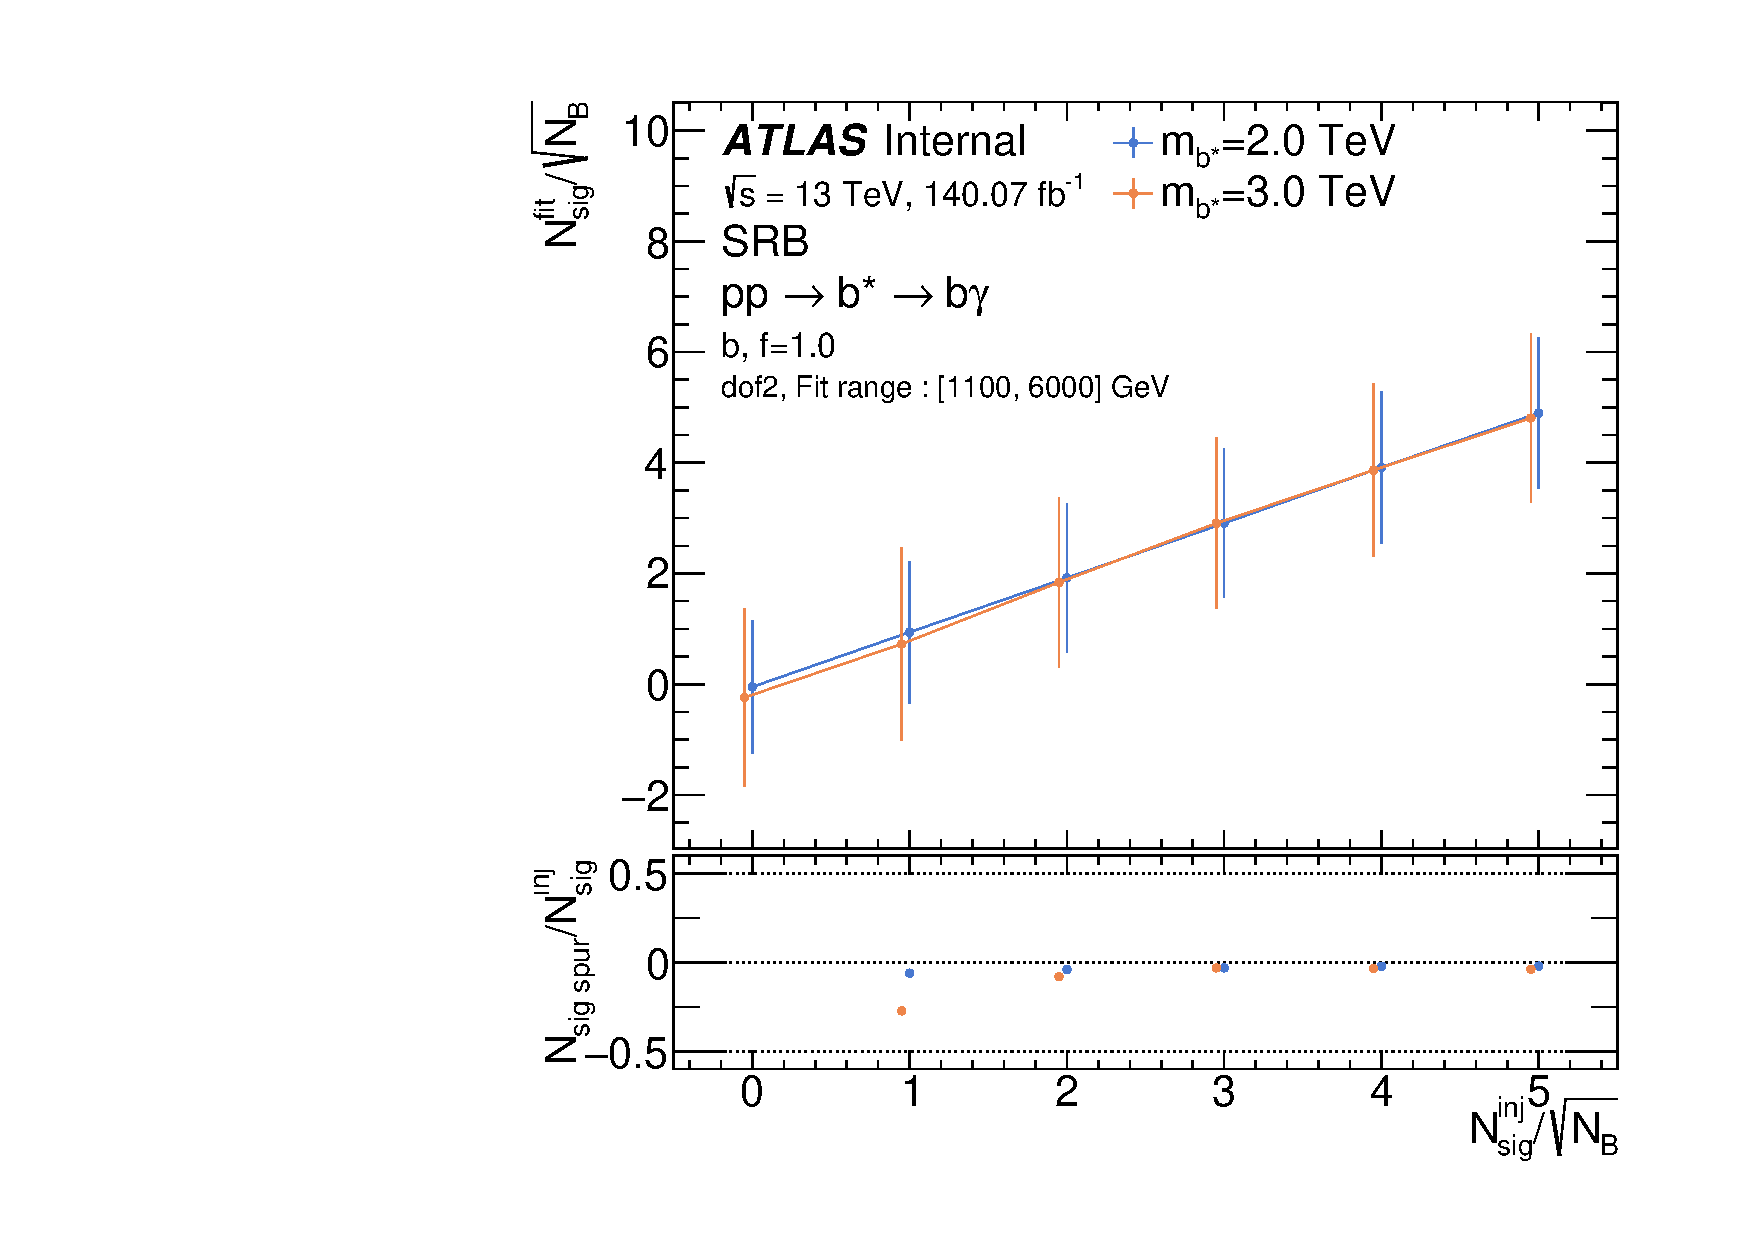
\includegraphics[width=\textwidth]{5_resonances/bkg/modeling/si/toys/SRB/qstar/b_1p00/dof2__range_1100_6000/plots/can__SigInj__photonjet_Pythia_jfakeisosmooth__qstar__SRB__b_1p00__dof2__range_1100_6000}
        \caption{SRB.}
    \end{subfigure}
    \hfill
    \begin{subfigure}[h]{0.49\linewidth}
        \centering
        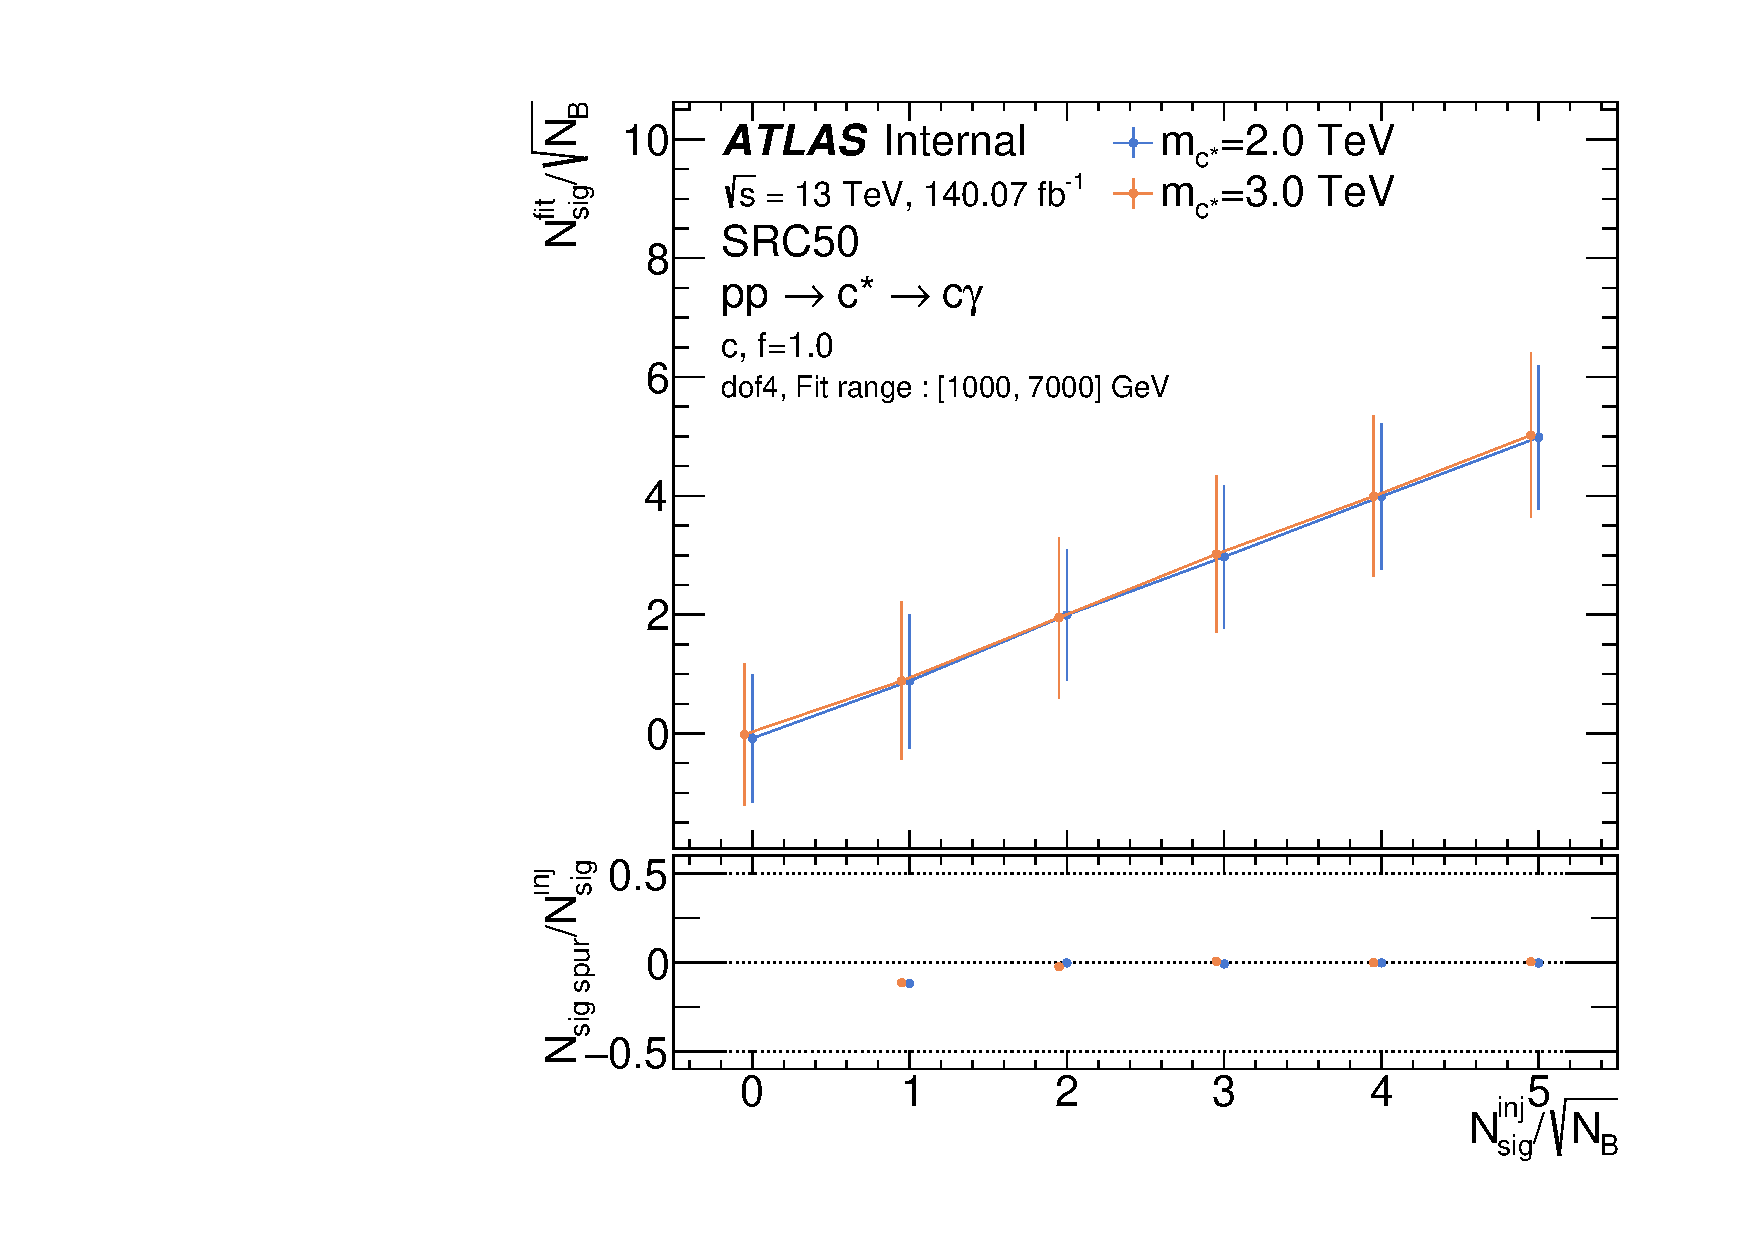
\includegraphics[width=\textwidth]{5_resonances/bkg/modeling/si/toys/SRC50/qstar/c_1p00/dof4__range_1000_7000/plots/can__SigInj__photonjet_Pythia_jfakeisosmooth__qstar__SRC50__c_1p00__dof4__range_1000_7000}
        \caption{SRC.}
    \end{subfigure}\\
    \caption{\ac{SI} tests for the \ac{EQ} model in regions SR, SRL, SRB and SRC, respectively. The fit-range and functional model used are the ones that yield the lowest \sspur, taken from the \ac{SSig} tests, and are displayed in each plot. Each considered mass is shown with a different color. The \(x\)-axis shows the injected amplitude in units of \(\sqrt{N_B}\), while the \(y\)-axis represents the extracted signal in terms of \(\sqrt{N_B}\).}
    \label{fig:bkg:modeling:sigbkg:sitest:siginj_qstar}
\end{figure}




% In \App{\ref{app:siginj_tests}} figures showing the Signal Injection tests presented, for the same combinations shown in \Tab{\ref{tab:bkg_modeling:ss_test:ss_ranking_SR}}. In all cases, the signal injection test is passed.
%%%%%%%%%%%%%%%%%%%%%%%%%%%%%%%%%%%%%%%%%%%%%%%%%%%%%%%%%%%%%%%%%%%%%%%%%%%%%%%%%%%%%%%%%%%%%%%%%%%%


%%%%%%%%%%%%%%%%%%%%%%%%%%%%%%%%%%%%%%%%%%%%%%%%%%%%%%%%%%%%%%%%%%%%%%%%%%%%%%%%%%%%%%%%%%%%%%%%%%%%
%%%%%%%%%%%%%%%%%%%%%%%%%%%%%%%%%%%%%%%%%%%%%%%%%%%%%%%%%%%%%%%%%%%%%%%%%%%%%%%%%%%%%%%%%%%%%%%%%%%%
%%%%%%%%%%%%%%%%%%%%%%%%%%%%%%%%%%%%%%%%%%%%%%%%%%%%%%%%%%%%%%%%%%%%%%%%%%%%%%%%%%%%%%%%%%%%%%%%%%%%



















%%%%%%%%%%%%%%%%%%%%%%%%%%%%%%%%%%%%%%%%%%%%%%%%%%%%%%%%%%%%%%%%%%%%%%%%%%%%%%%%%%%%%%%%%%%%%%%%%%%%
\subsubsection{\(F\)-tests}
\label{subsubsec:bkg:modeling:preparation:ftest}

Once the optimal fit-range and a function ranking has been set by virtue of the \ac{SSig} tests, the final statistical test to select the function is the \(F\)-test. The test compares fits done with a function \(a\) with \(p_a = n\) parameters with another function \(b\) which has \(p_b = n+1\) parameters. For the \(F\)-test, model \(a\) is a subset of model \(b\). In this test, a test statistic \(F\) is computed from the resulting \chisq values::
\begin{equation}
    \label{eq:bkg:modeling:preparation:ftest:ftest}
    F = \frac{
        \displaystyle
        \frac{\chisq_a - \chisq_b}{p_b - p_a}
    }{
        \displaystyle
        \frac{\chisq_b}{N - p_b}
    },
\end{equation}
where \(N\) is the total number of bins in the sample.
High values of \(F\) mean that the model with \(n\) parameters should be discarded, while cases in which \(F \to 0\) (\(\chisq_a - \chisq_b \to 0\)), the difference between the models is not significant, leading to select the model with the lowest amount of parameters, i.e model \(a\) with \(n\) parameters.

% To compute this values, toys generated from the \textit{dof7} distribution are fitted with the \textit{dof(2-6)} functions. For each same toy, the \(F\)-value shown in \Eqn{\ref{eq:bkg:modeling:preparation:ftest:ftest}} is computed where function \(a\) represents the \textit{dofn} function and \(b\) the \textit{dof(n+1)} function.


The null hypothesis is defined as the one in which model \(b\) does not provide a better significant difference compared to model \(a\) (small \(F\)), and in this situation, \(F\) will have an \(F\)-distribution with \((p_b - p_a, N - p_b)\) \ac{dof}. The null hypothesis is rejected if the \(F\)-score is higher than a critical value, usually set to that leading to a p-value \(p\left(F(p_b-p_a, N-p_b)\right)<0.05\). In summary, if the p-value of comparing model \(a\) and \(b\) is \(>0.05\), the null hypothesis is not rejected, and the two models are considered similar, while p-values \(<0.05\) mean that there is evidence against the null hypothesis, and the more simple model \(a\) is rejected.
For the study of selecting the best fit function, model \(a\) is the nominal function with \textit{dofn} and model \(b\) is the alternate function \textit{dof(n+1)}.

Fits are done to toys drawn from the \textit{dof7} fit to the \ac{BO} \ac{MC} Asimov distribution. The selected fit ranges for these studies are the ones decided based on the previous \ac{SSig} test. Model \(a\) and \(b\) are fitted to the same toy, and they are compared if and only if both of the fits converge. For each one of the toys, the \(F\)-value is calculated according to \Eqn{\ref{eq:bkg:modeling:preparation:ftest:ftest}}, and finally, the p-value \pzero.
% Similarly, fits are also done to MC Asimov datasets using different models. In these cases, a single set of \(F\)- and p-values is obtained for each signal region.


\begin{figure}[ht!]
    \centering
    \begin{subfigure}[h]{0.49\linewidth}
        \centering
        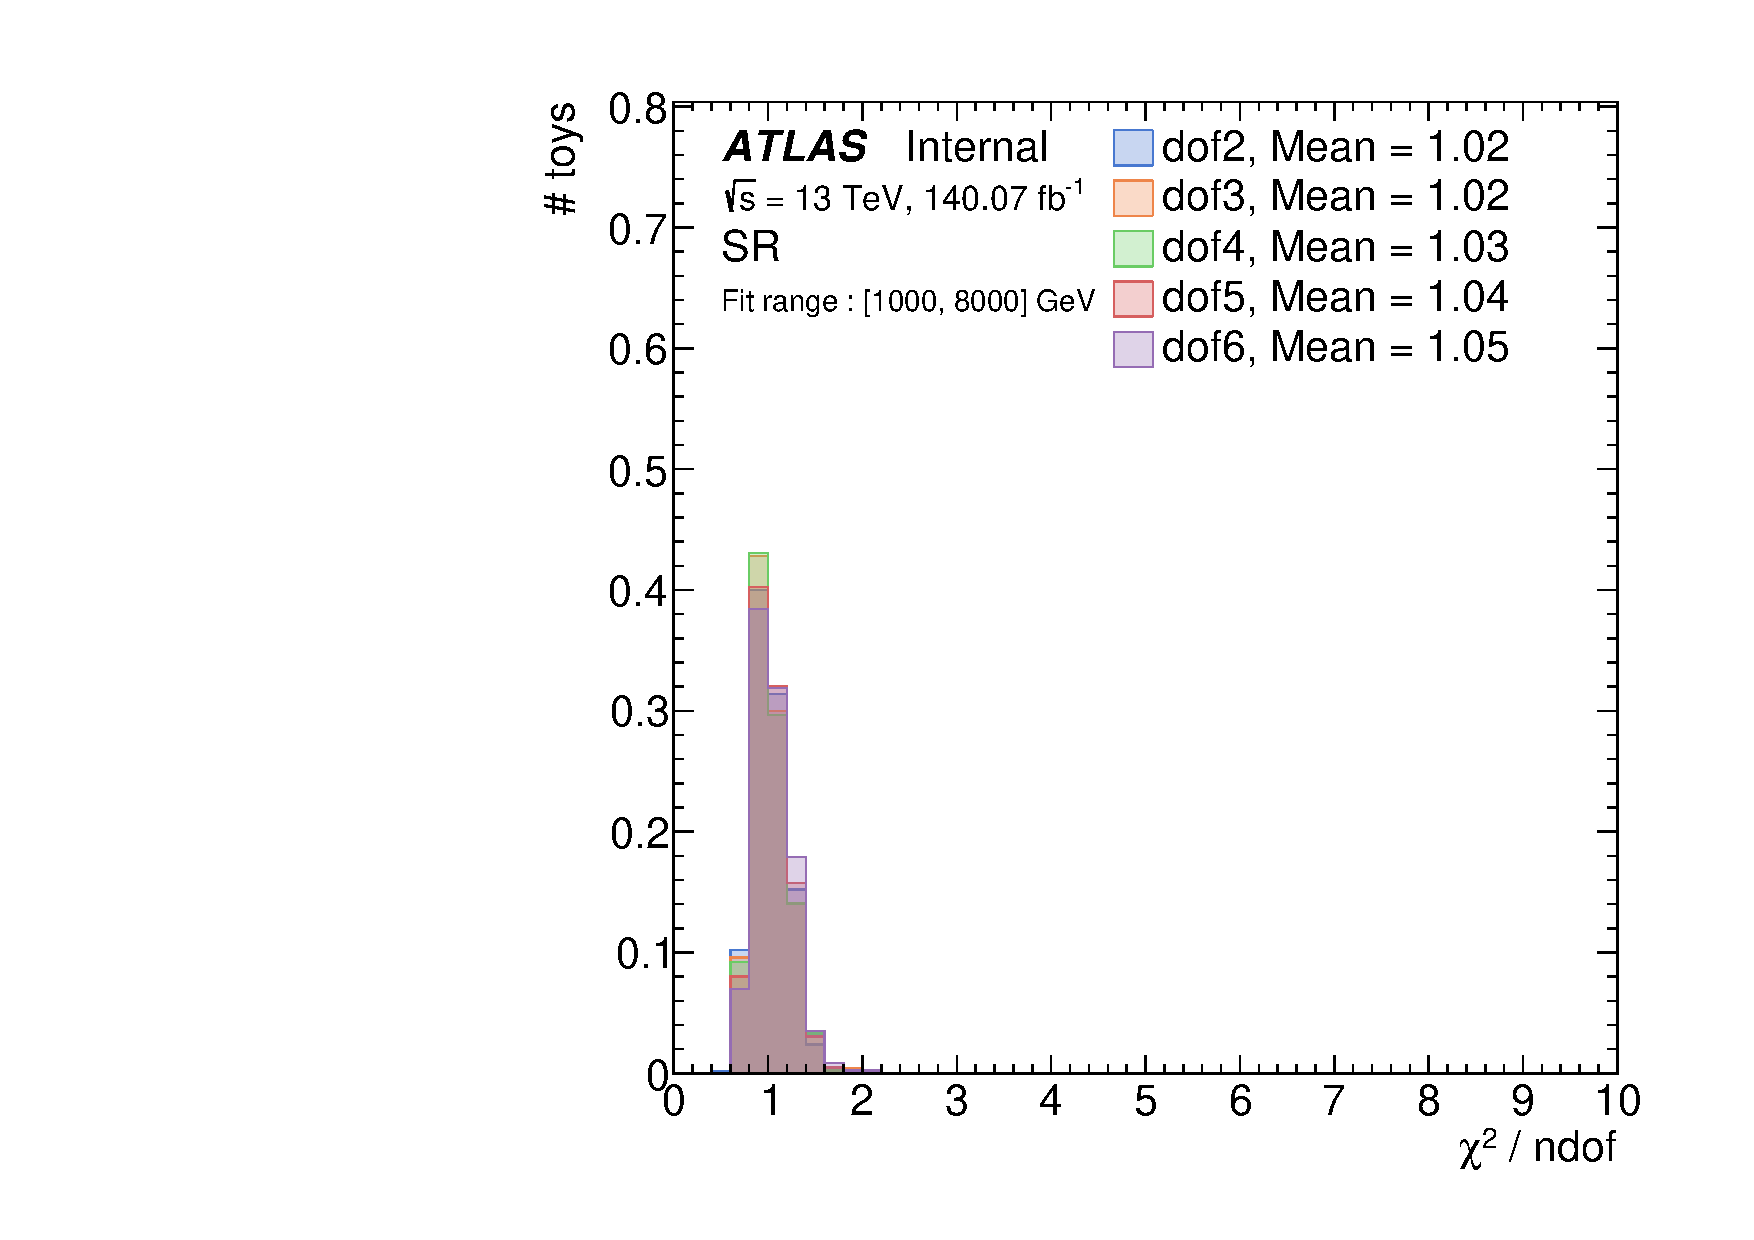
\includegraphics[width=0.8\textwidth]{5_resonances/bkg/modeling/ftest/SR/can__photonjet_Pythia_jfakeisosmooth__SR__chi2ndof__range_1000_8000__toys}
        \caption{SR}
    \end{subfigure}
    \begin{subfigure}[h]{0.49\linewidth}
        \centering
        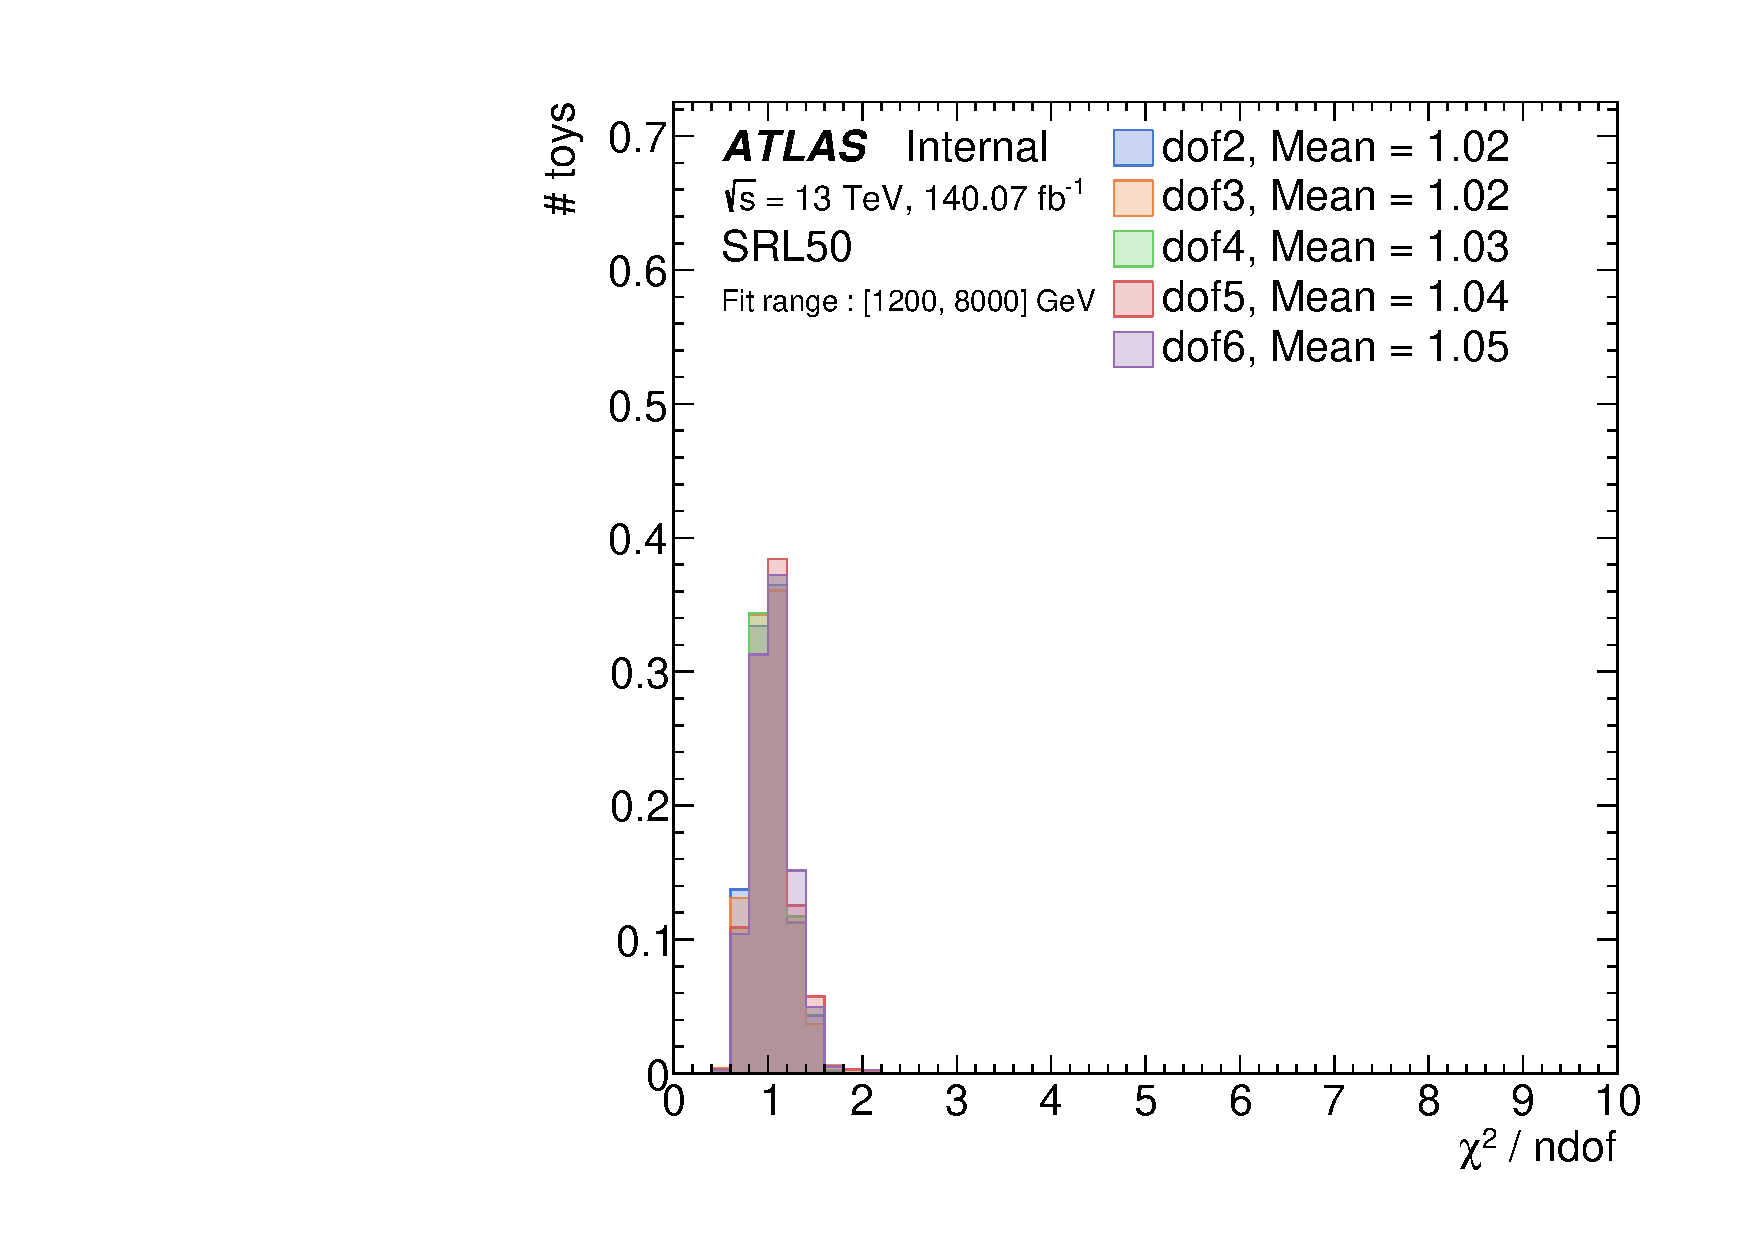
\includegraphics[width=0.8\textwidth]{5_resonances/bkg/modeling/ftest/SRL50/can__photonjet_Pythia_jfakeisosmooth__SRL50__chi2ndof__range_1200_8000__toys}
        \caption{SRL}
    \end{subfigure}
    \\
    \begin{subfigure}[h]{0.49\linewidth}
        \centering
        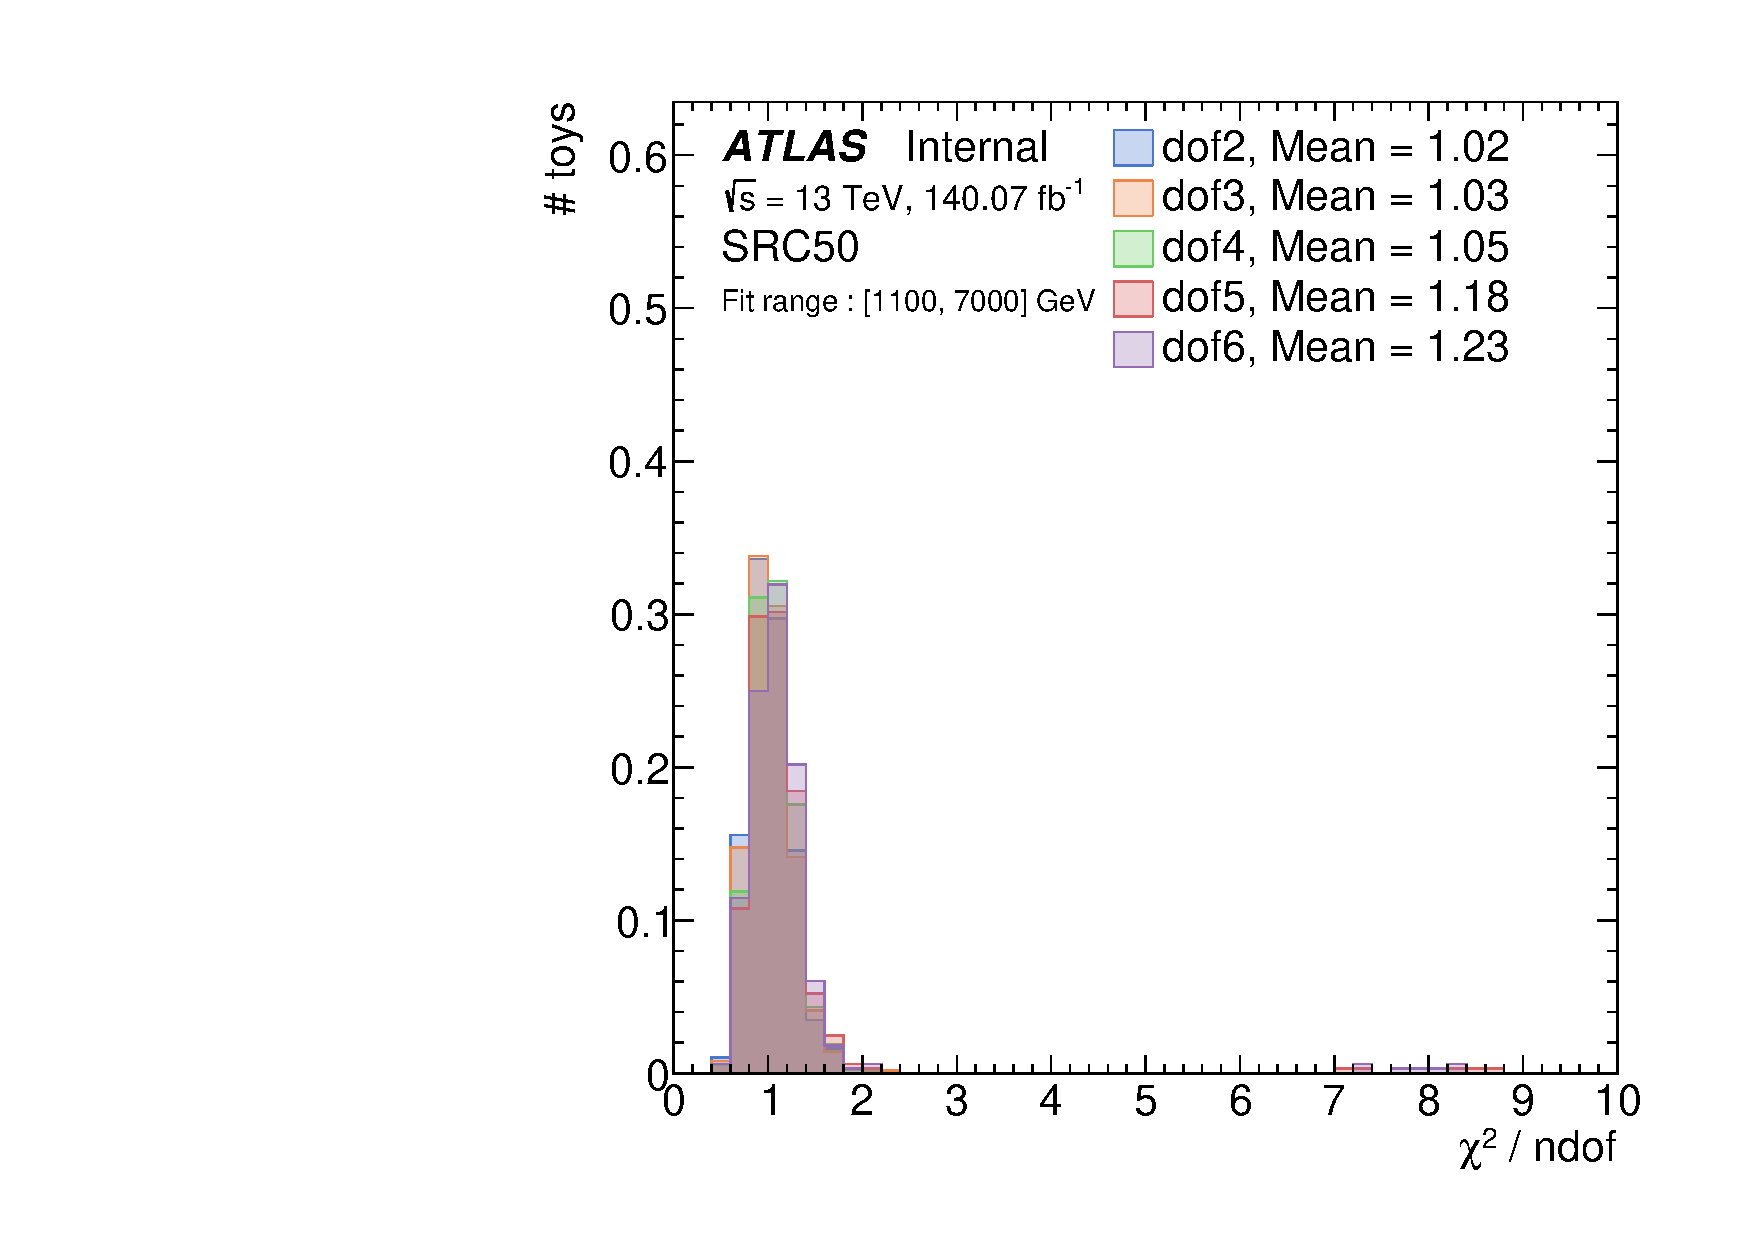
\includegraphics[width=0.8\textwidth]{5_resonances/bkg/modeling/ftest/SRC50/can__photonjet_Pythia_jfakeisosmooth__SRC50__chi2ndof__range_1100_7000__toys}
        \caption{SRC}
    \end{subfigure}
    \begin{subfigure}[h]{0.49\linewidth}
        \centering
        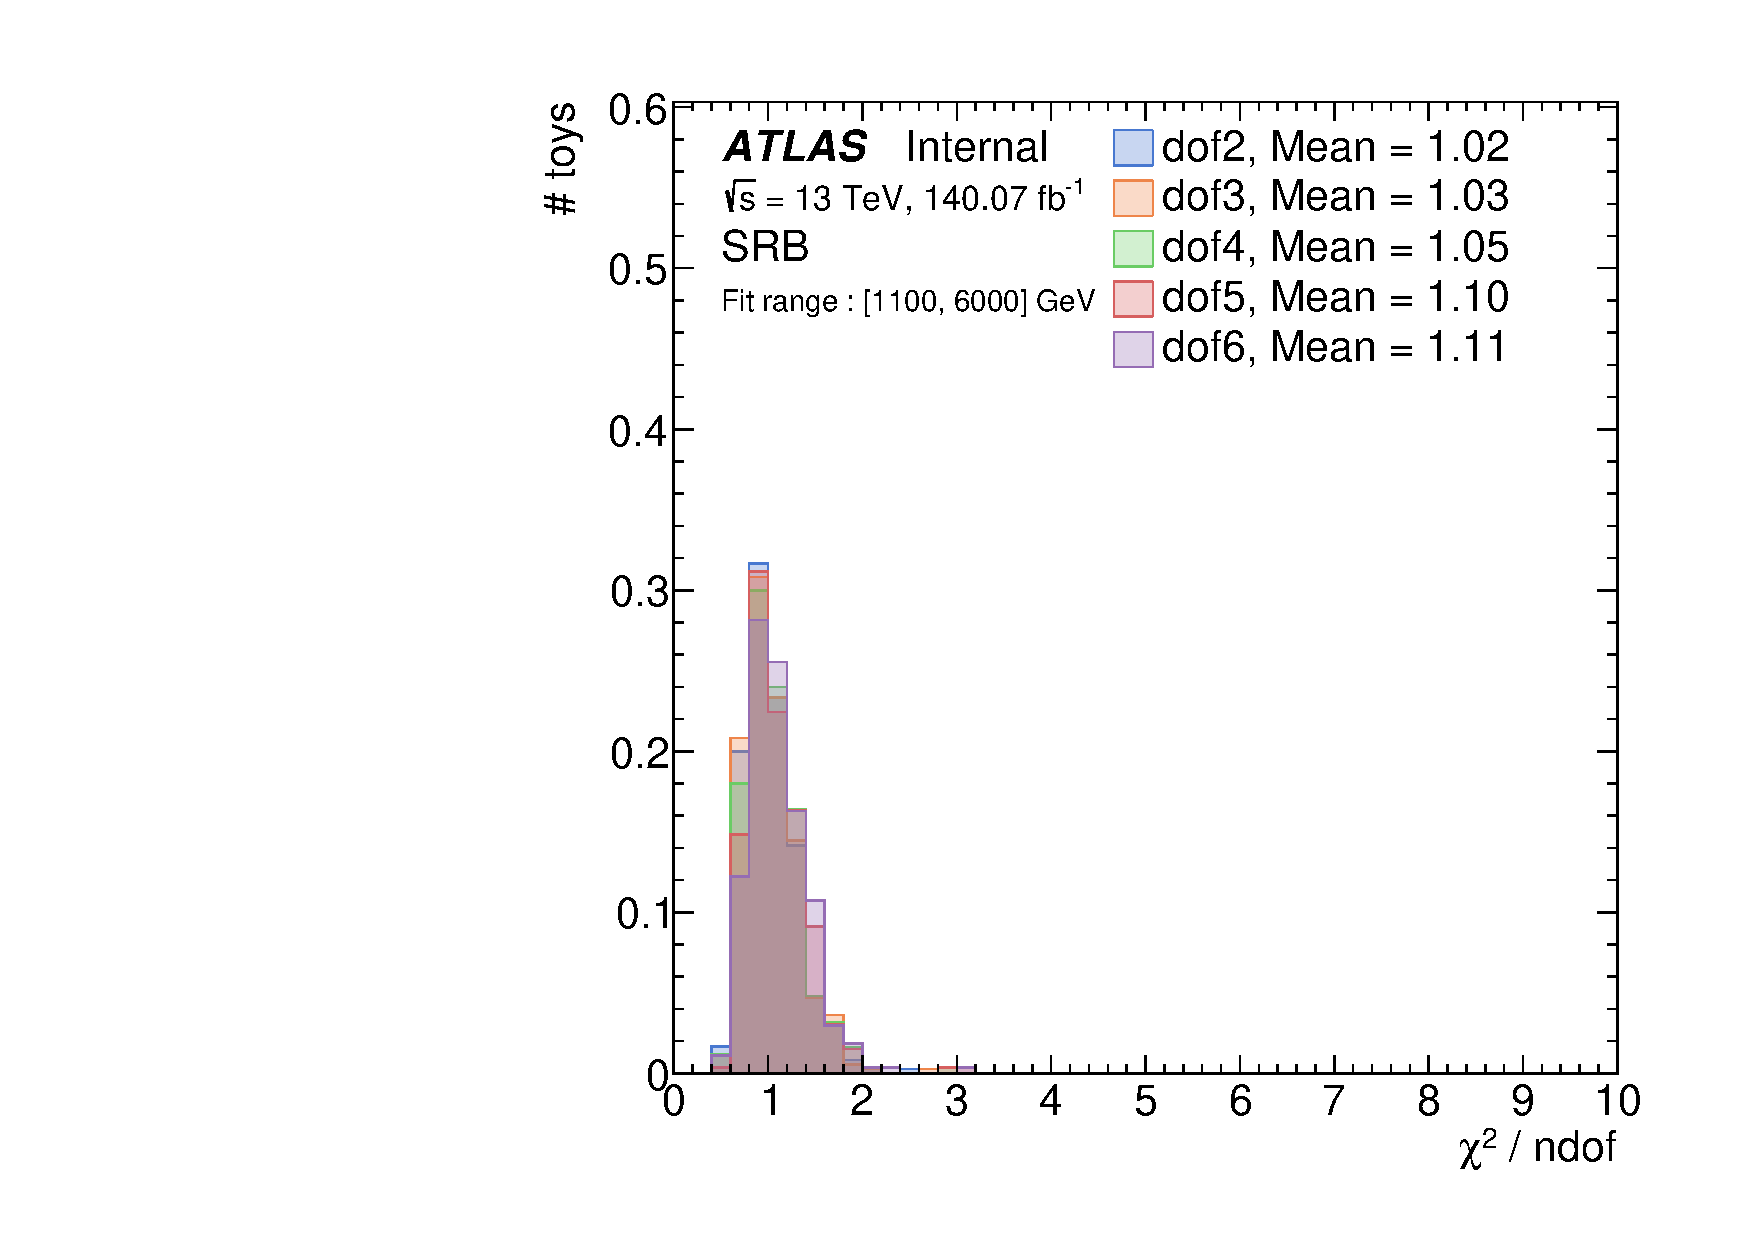
\includegraphics[width=0.8\textwidth]{5_resonances/bkg/modeling/ftest/SRB/can__photonjet_Pythia_jfakeisosmooth__SRB__chi2ndof__range_1100_6000__toys}
        \caption{SRB}
    \end{subfigure}
    \caption{\(\chisq / \text{ndof}\) distribution for each functional model in different signal regions.}
    \label{fig:bkg:modeling:preparation:ftest:chi2ndof}
\end{figure}

\begin{figure}[ht!]
    \centering
    \begin{subfigure}[h]{0.49\linewidth}
        \centering
        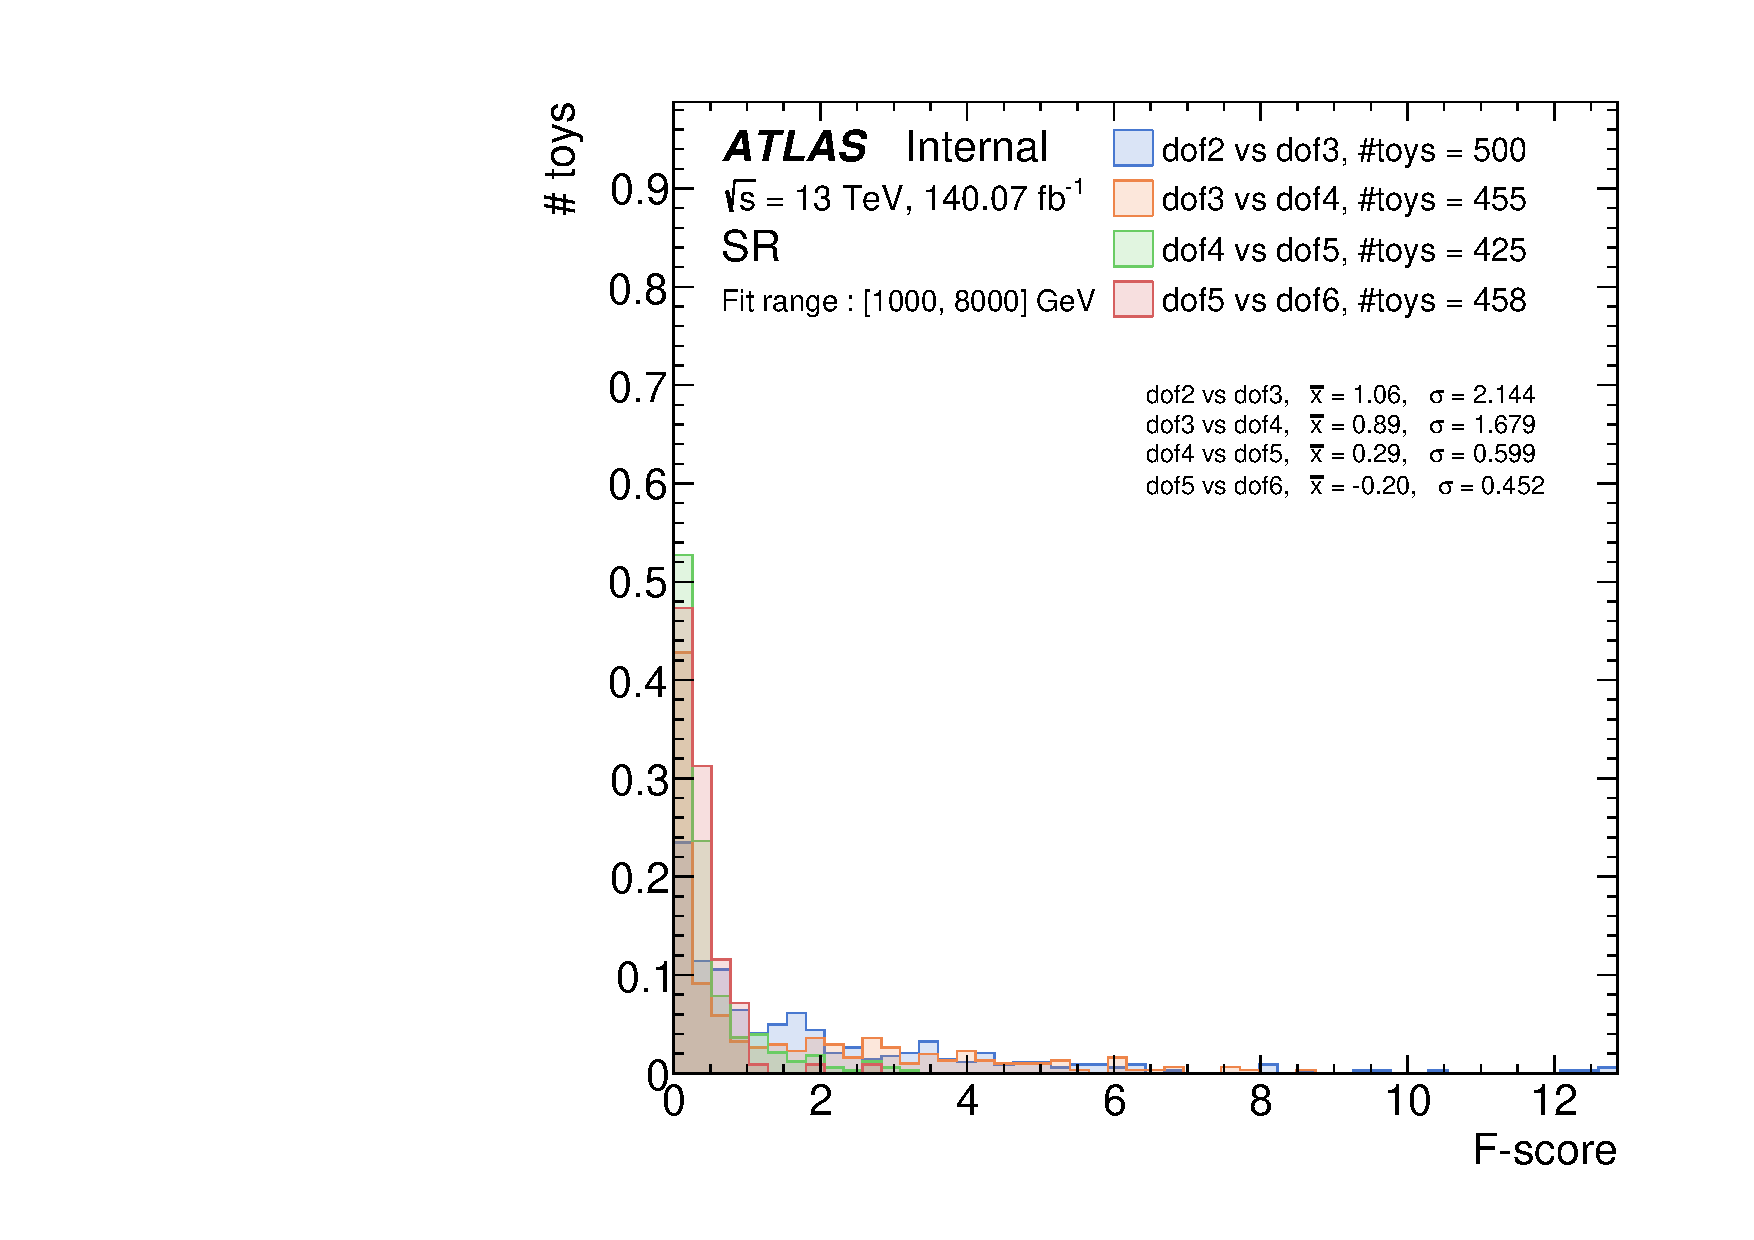
\includegraphics[width=0.8\textwidth]{5_resonances/bkg/modeling/ftest/SR/can__photonjet_Pythia_jfakeisosmooth__SR__fvalue__range_1000_8000__toys}
        \caption{SR}
    \end{subfigure}
    \begin{subfigure}[h]{0.49\linewidth}
        \centering
        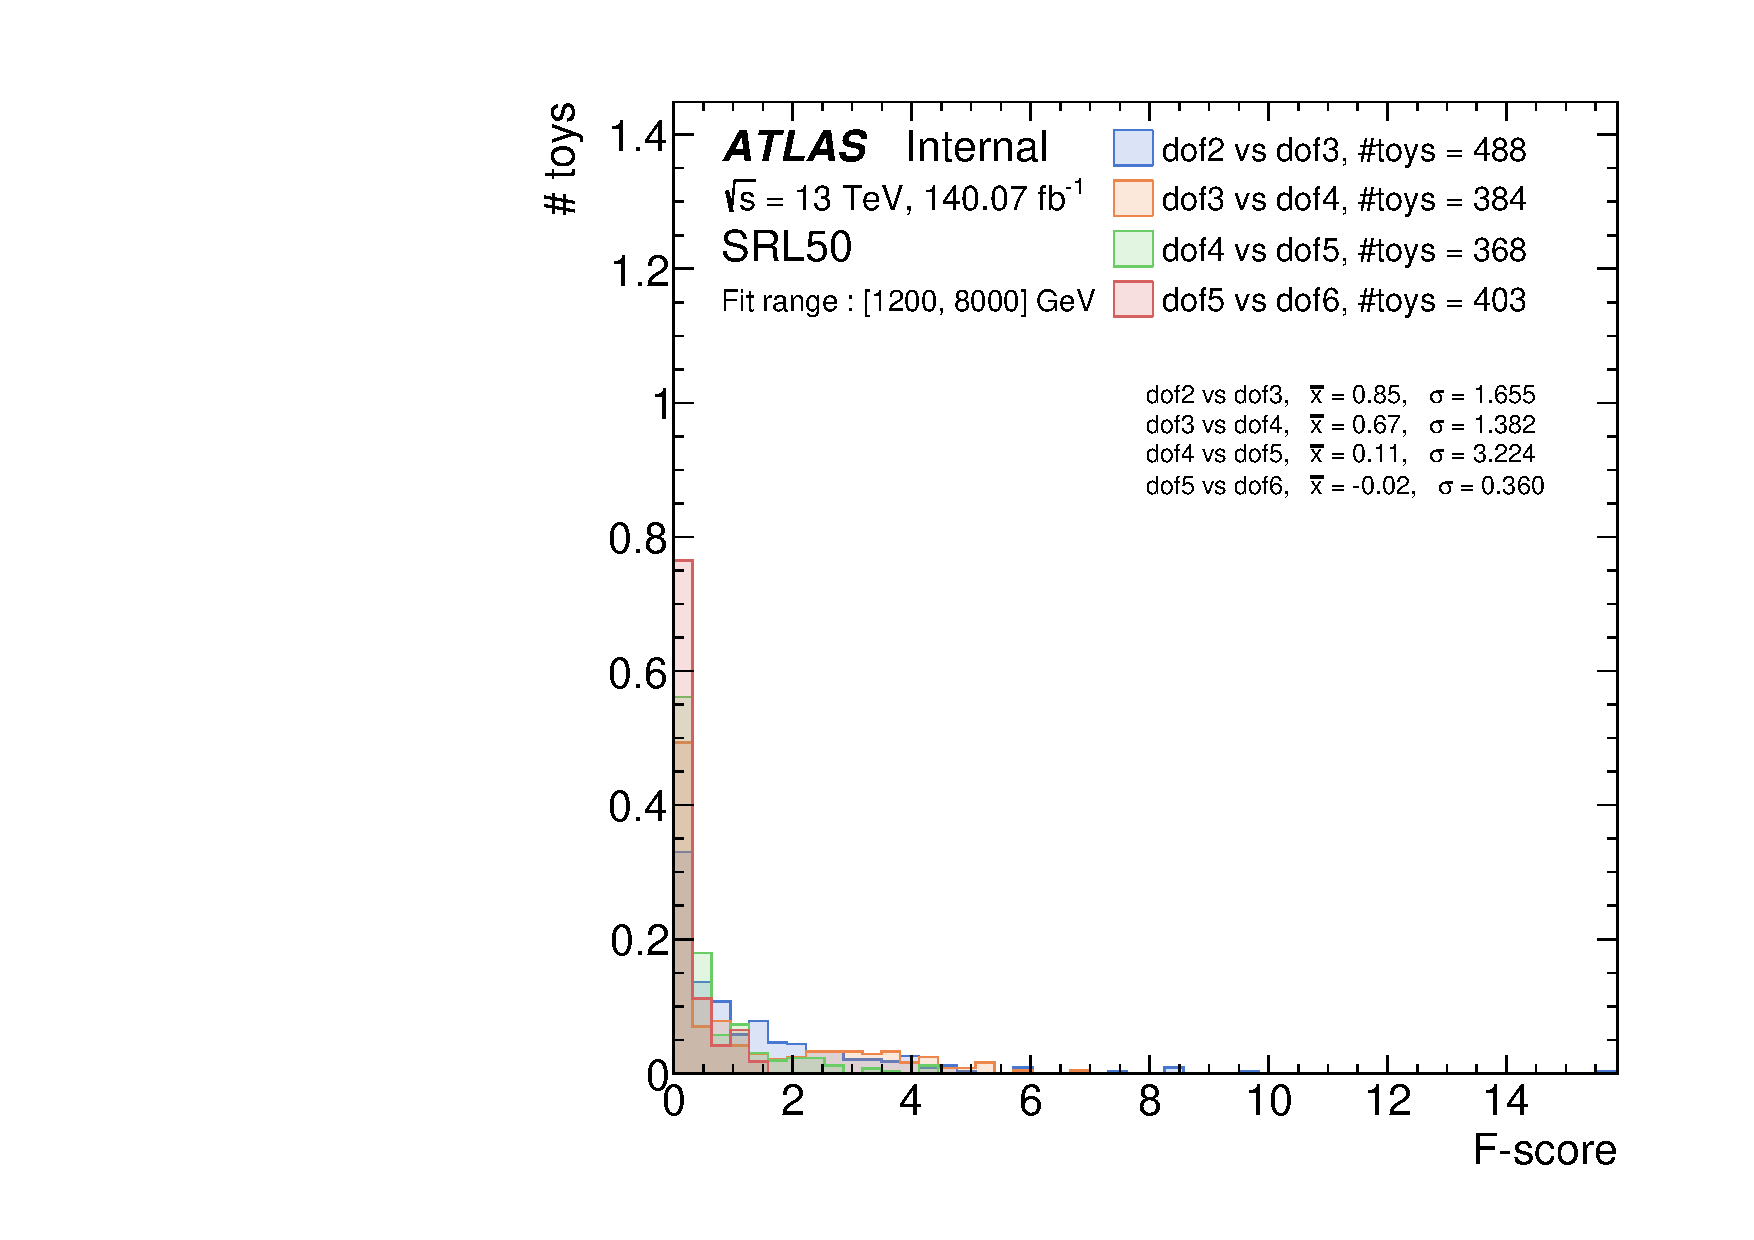
\includegraphics[width=0.8\textwidth]{5_resonances/bkg/modeling/ftest/SRL50/can__photonjet_Pythia_jfakeisosmooth__SRL50__fvalue__range_1200_8000__toys}
        \caption{SRL}
    \end{subfigure}
    \\
    \begin{subfigure}[h]{0.49\linewidth}
        \centering
        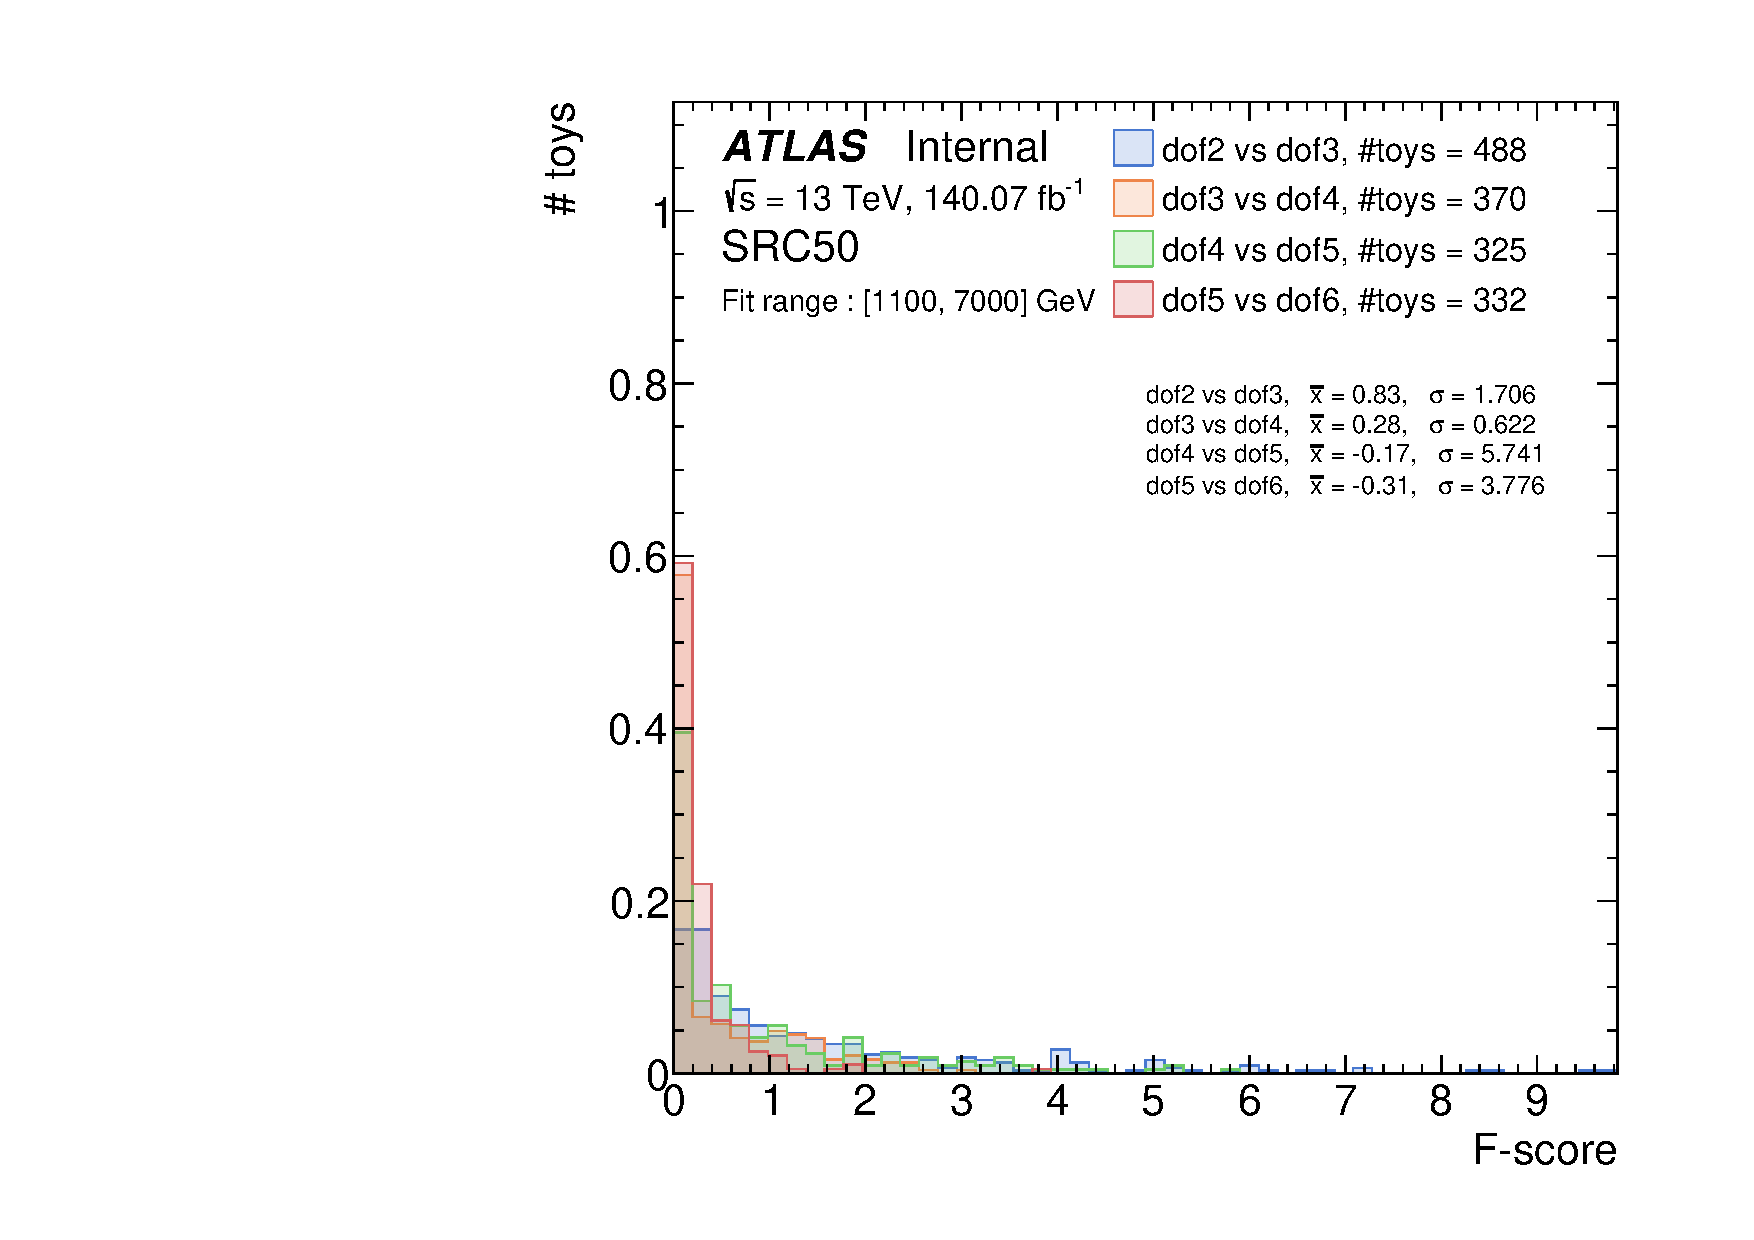
\includegraphics[width=0.8\textwidth]{5_resonances/bkg/modeling/ftest/SRC50/can__photonjet_Pythia_jfakeisosmooth__SRC50__fvalue__range_1100_7000__toys}
        \caption{SRC}
    \end{subfigure}
    \begin{subfigure}[h]{0.49\linewidth}
        \centering
        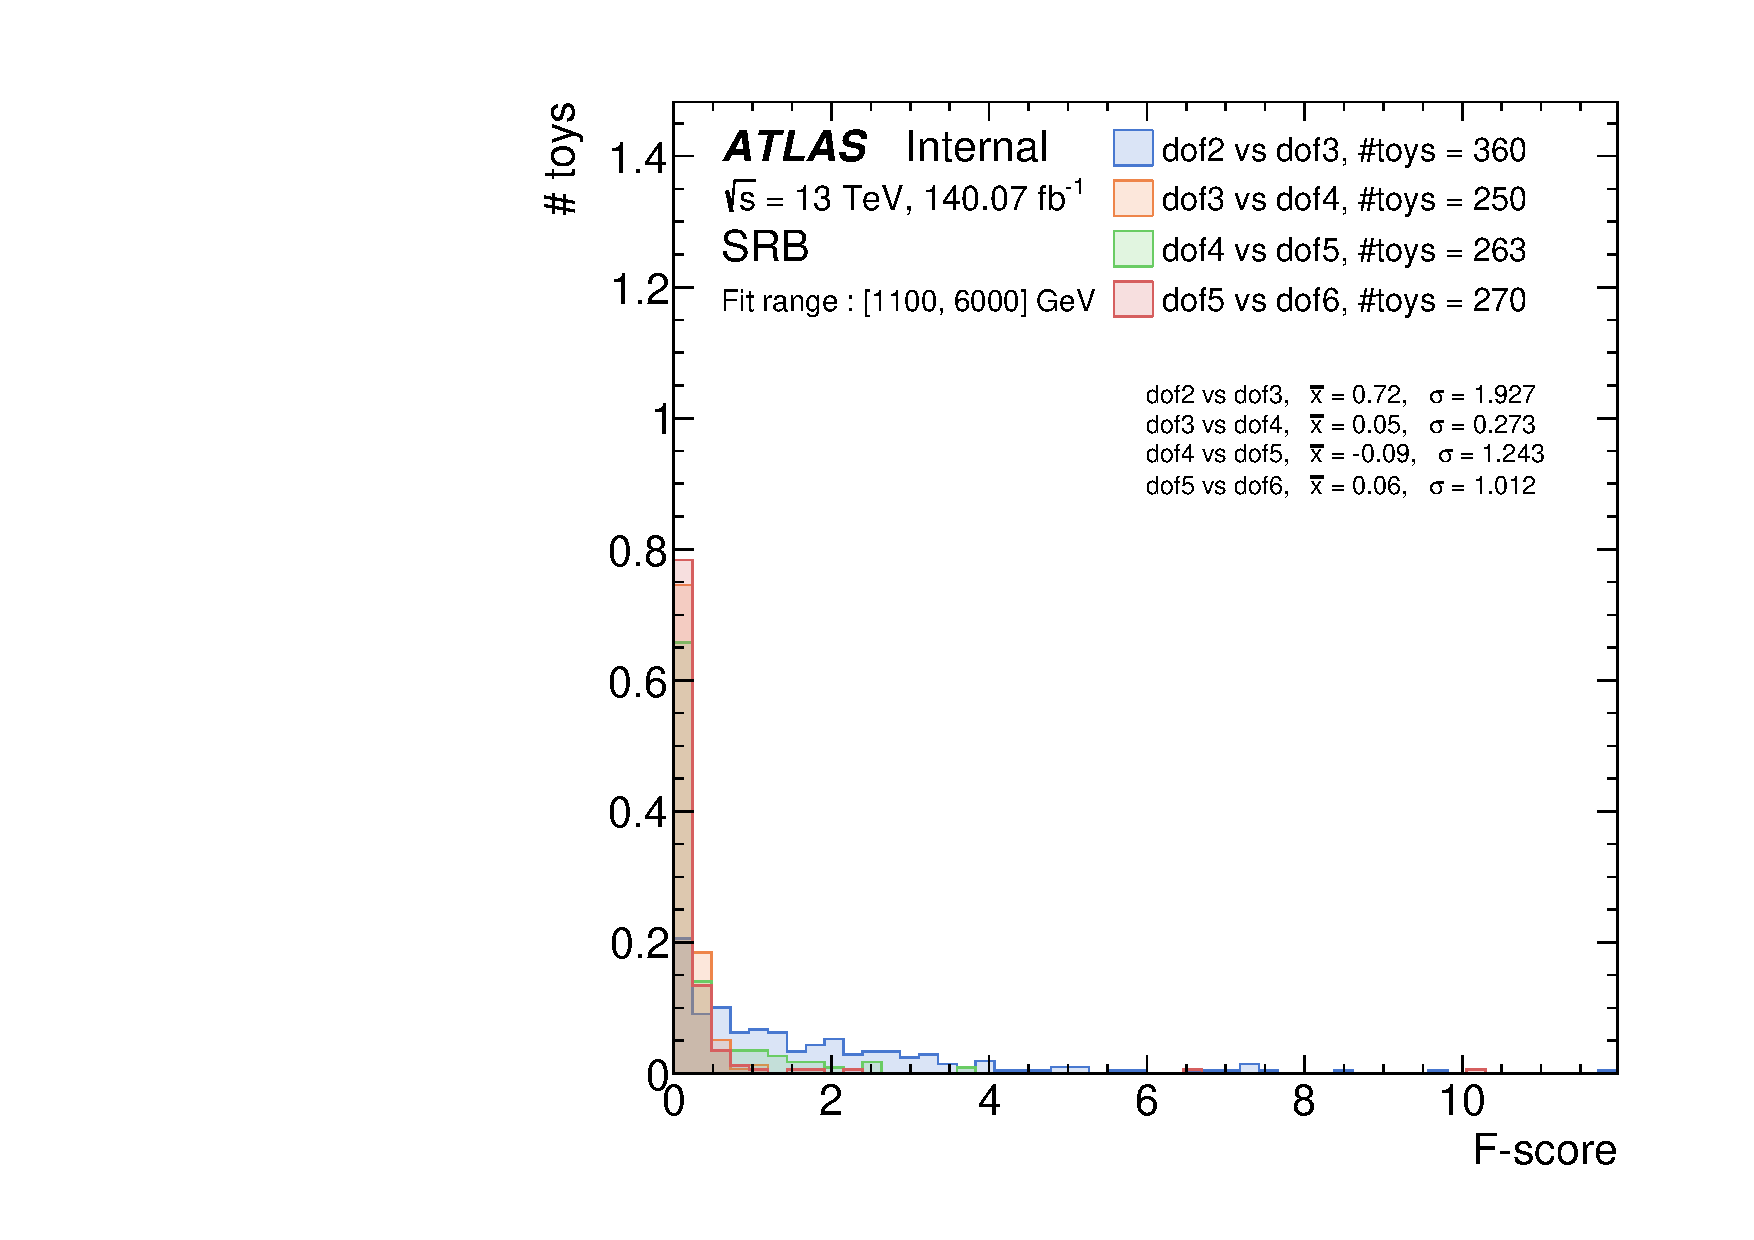
\includegraphics[width=0.8\textwidth]{5_resonances/bkg/modeling/ftest/SRB/can__photonjet_Pythia_jfakeisosmooth__SRB__fvalue__range_1100_6000__toys}
        \caption{SRB}
    \end{subfigure}
    \caption{\(F\)-score distribution. The tests are done by comparing two functional models at the same time, shown by each of the filled histograms. For each one of them, the number of matching and converged, toys are shown, as are the means and widths of the \(F\)-score distributions.}
    \label{fig:bkg:modeling:preparation:ftest:ftest}
\end{figure}

\begin{figure}[ht!]
    \centering
    \begin{subfigure}[h]{0.49\linewidth}
        \centering
        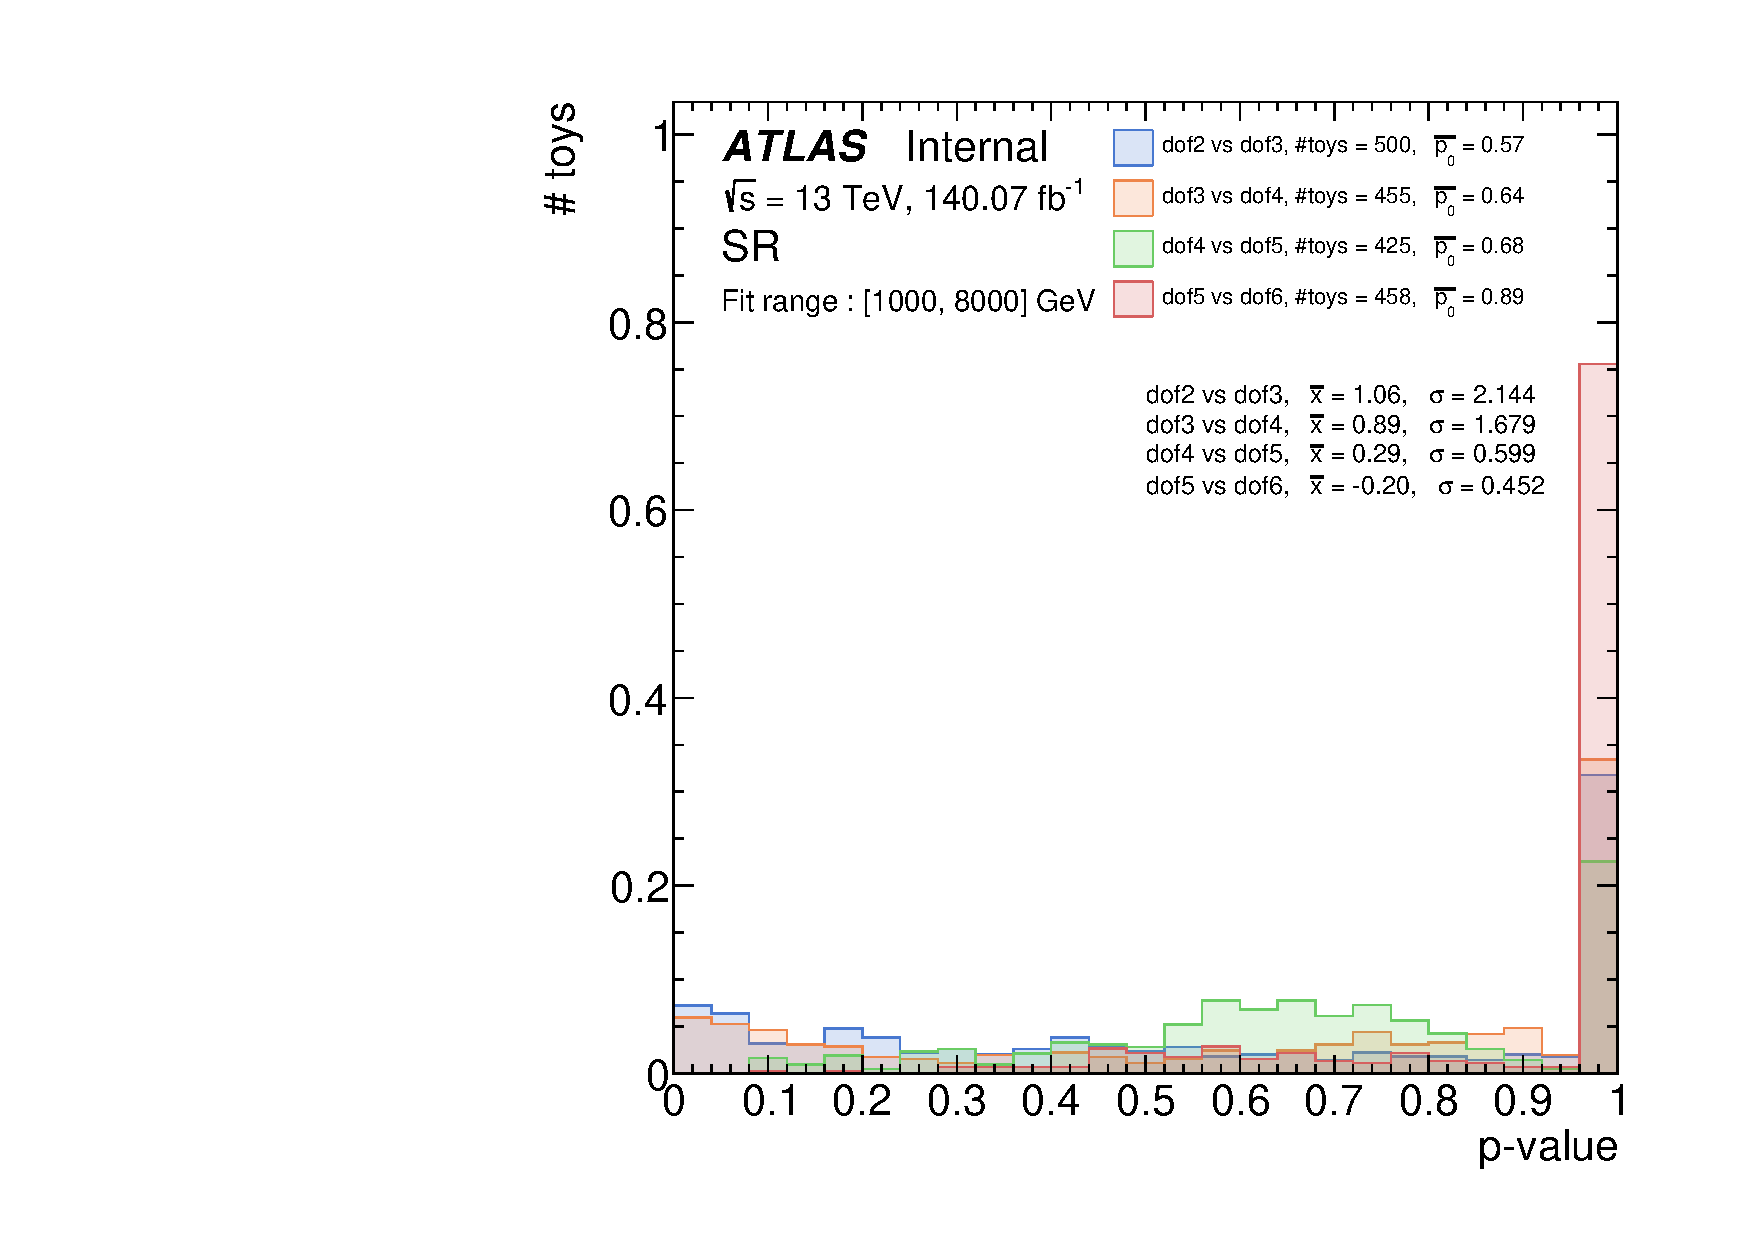
\includegraphics[width=0.8\textwidth]{5_resonances/bkg/modeling/ftest/SR/can__photonjet_Pythia_jfakeisosmooth__SR__fvalue_pvalue__range_1000_8000__toys}
        \caption{SR}
    \end{subfigure}
    \begin{subfigure}[h]{0.49\linewidth}
        \centering
        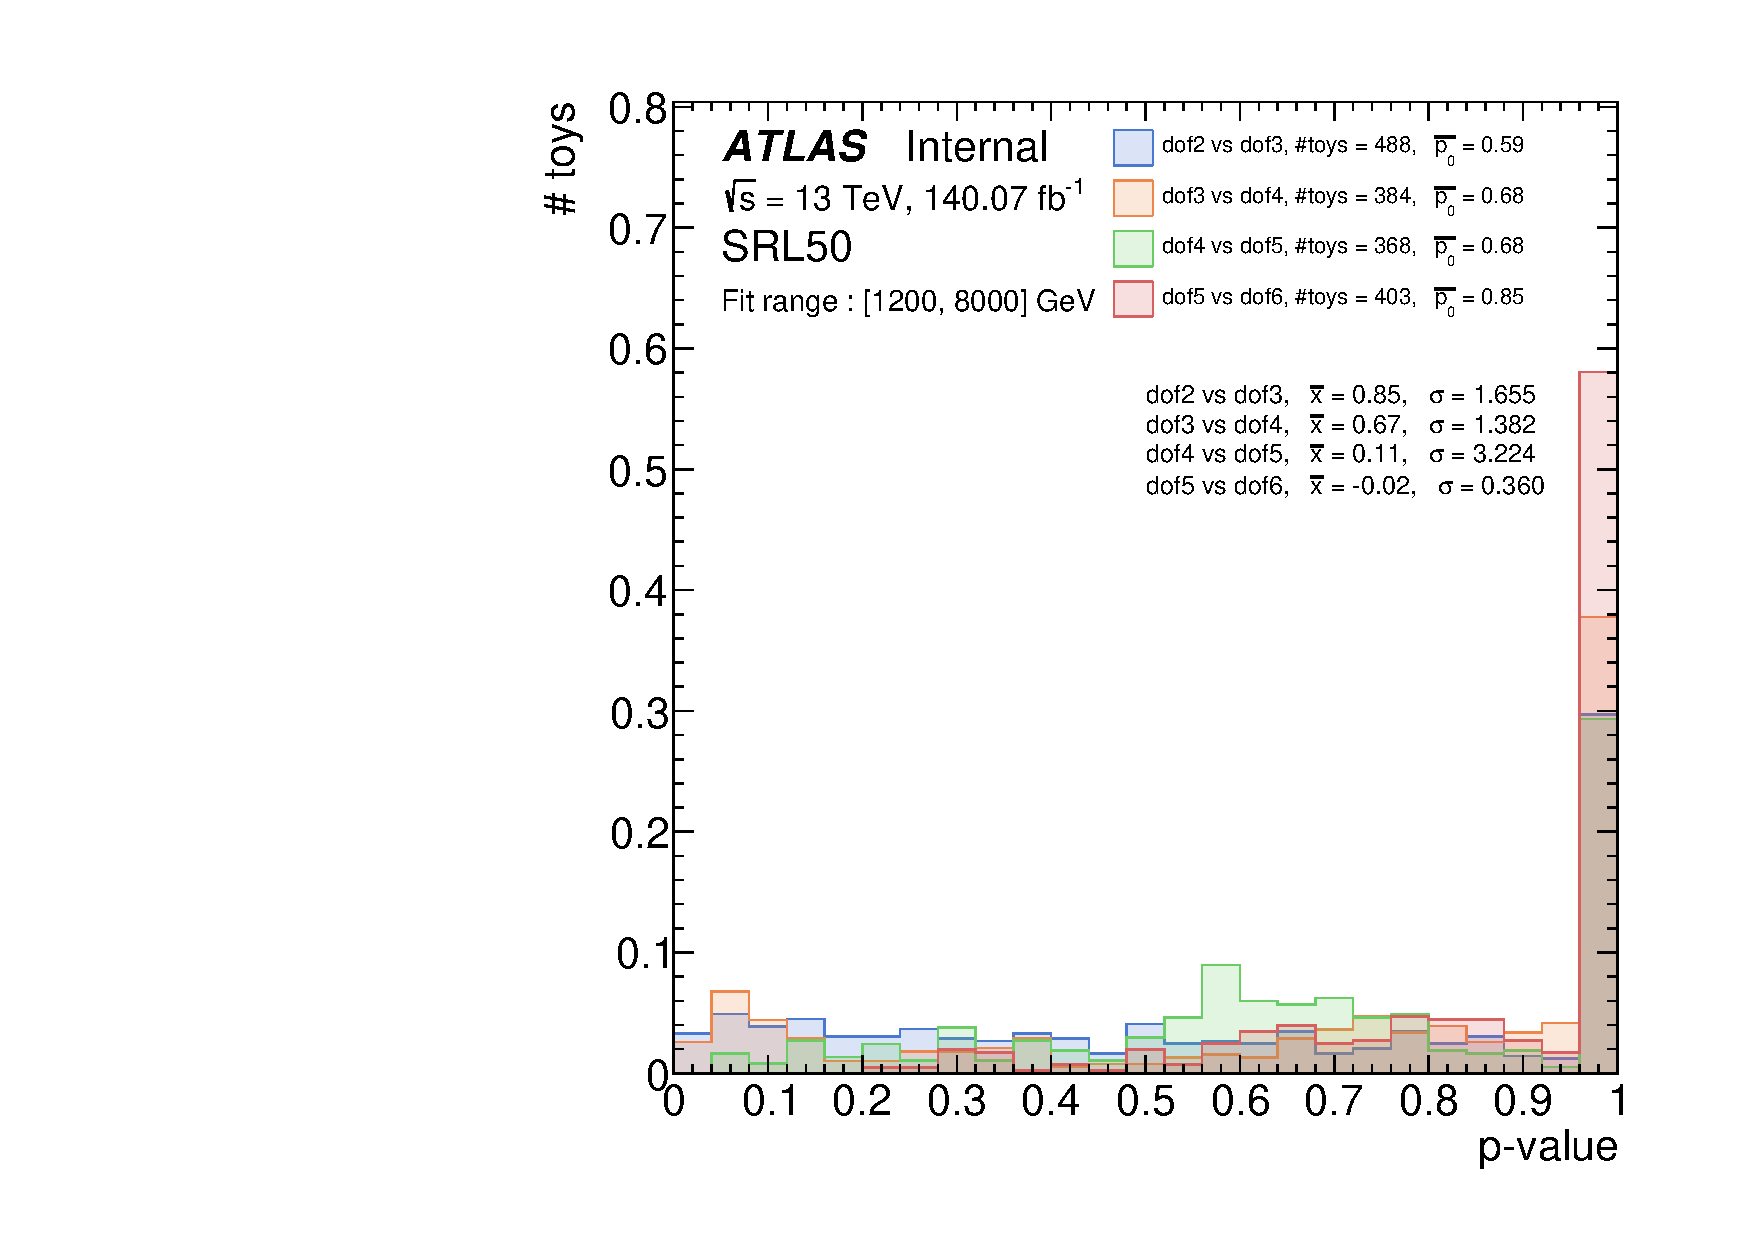
\includegraphics[width=0.8\textwidth]{5_resonances/bkg/modeling/ftest/SRL50/can__photonjet_Pythia_jfakeisosmooth__SRL50__fvalue_pvalue__range_1200_8000__toys}
        \caption{SRL}
    \end{subfigure}
    \\
    \begin{subfigure}[h]{0.49\linewidth}
        \centering
        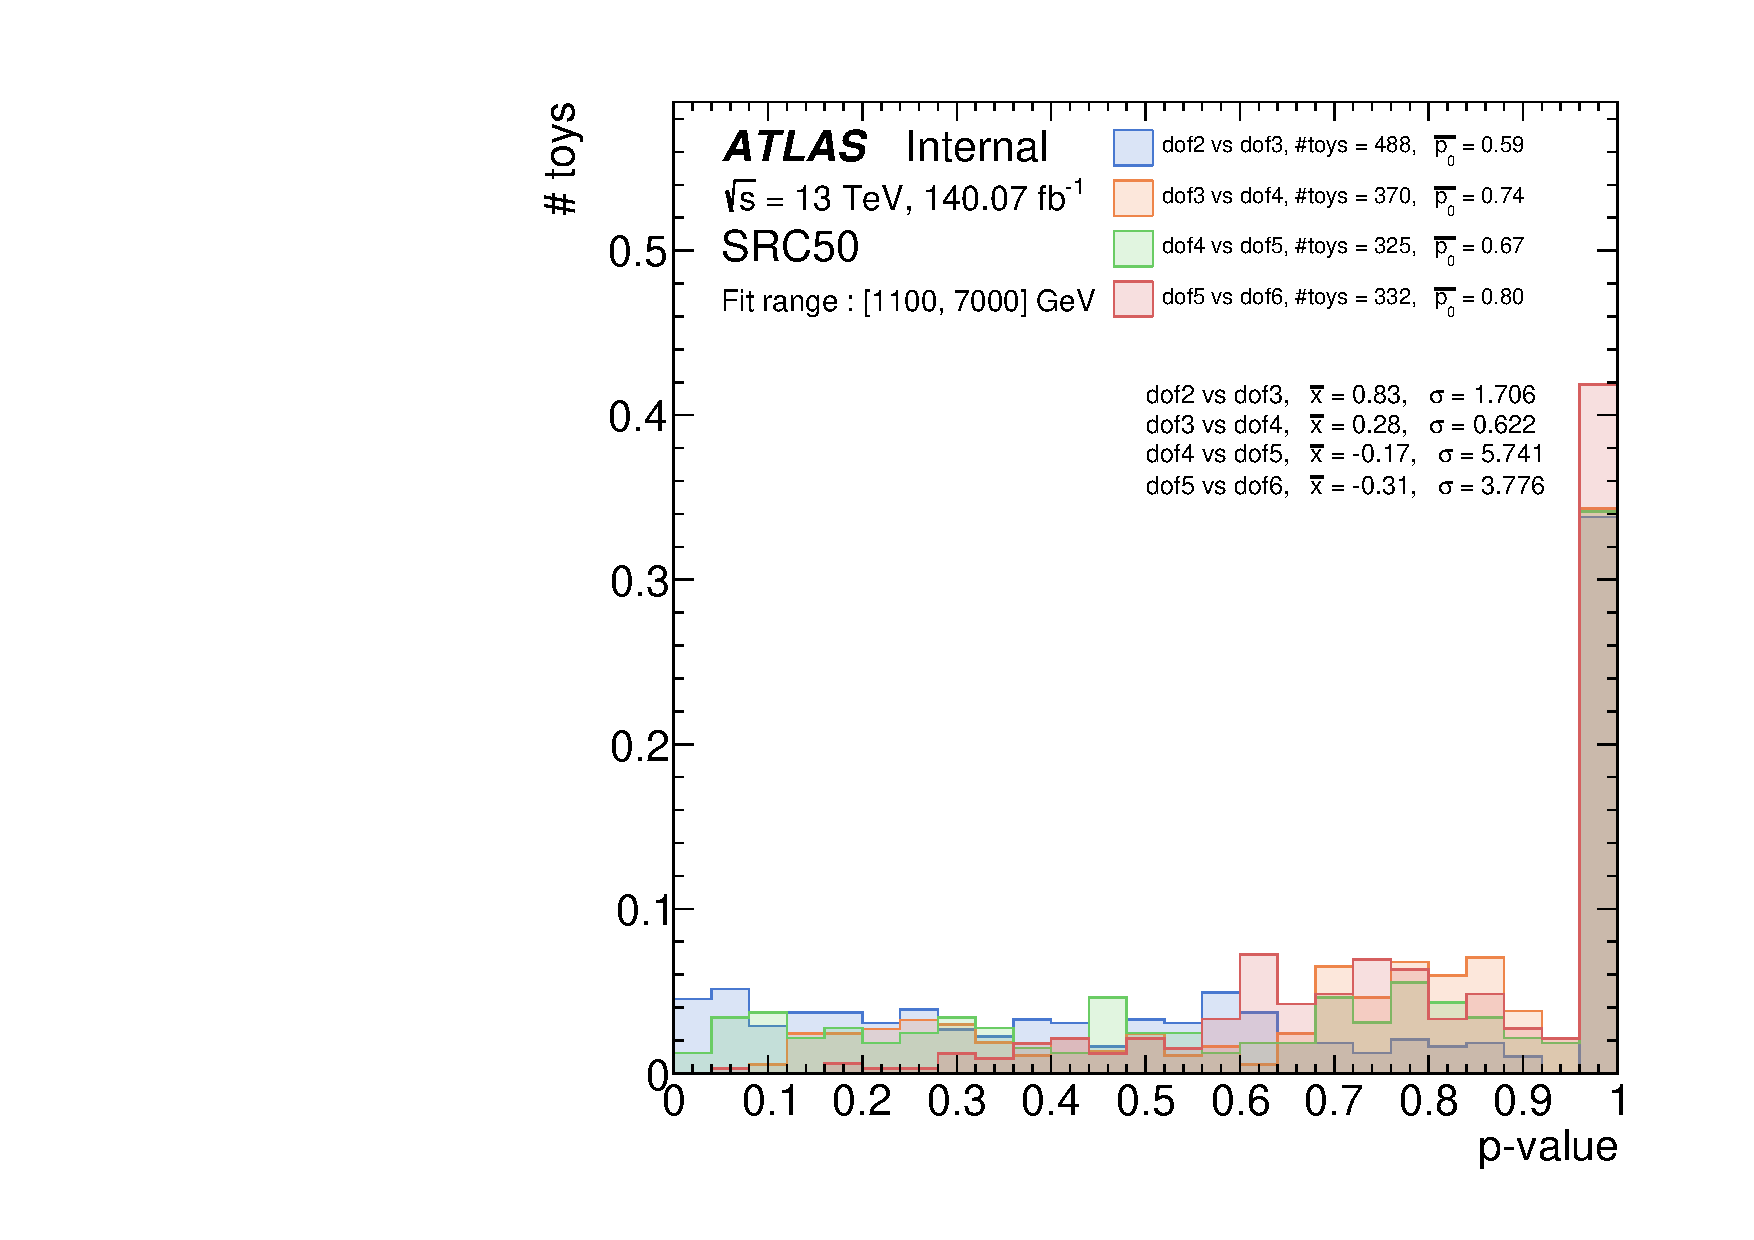
\includegraphics[width=0.8\textwidth]{5_resonances/bkg/modeling/ftest/SRC50/can__photonjet_Pythia_jfakeisosmooth__SRC50__fvalue_pvalue__range_1100_7000__toys}
        \caption{SRC}
    \end{subfigure}
    \begin{subfigure}[h]{0.49\linewidth}
        \centering
        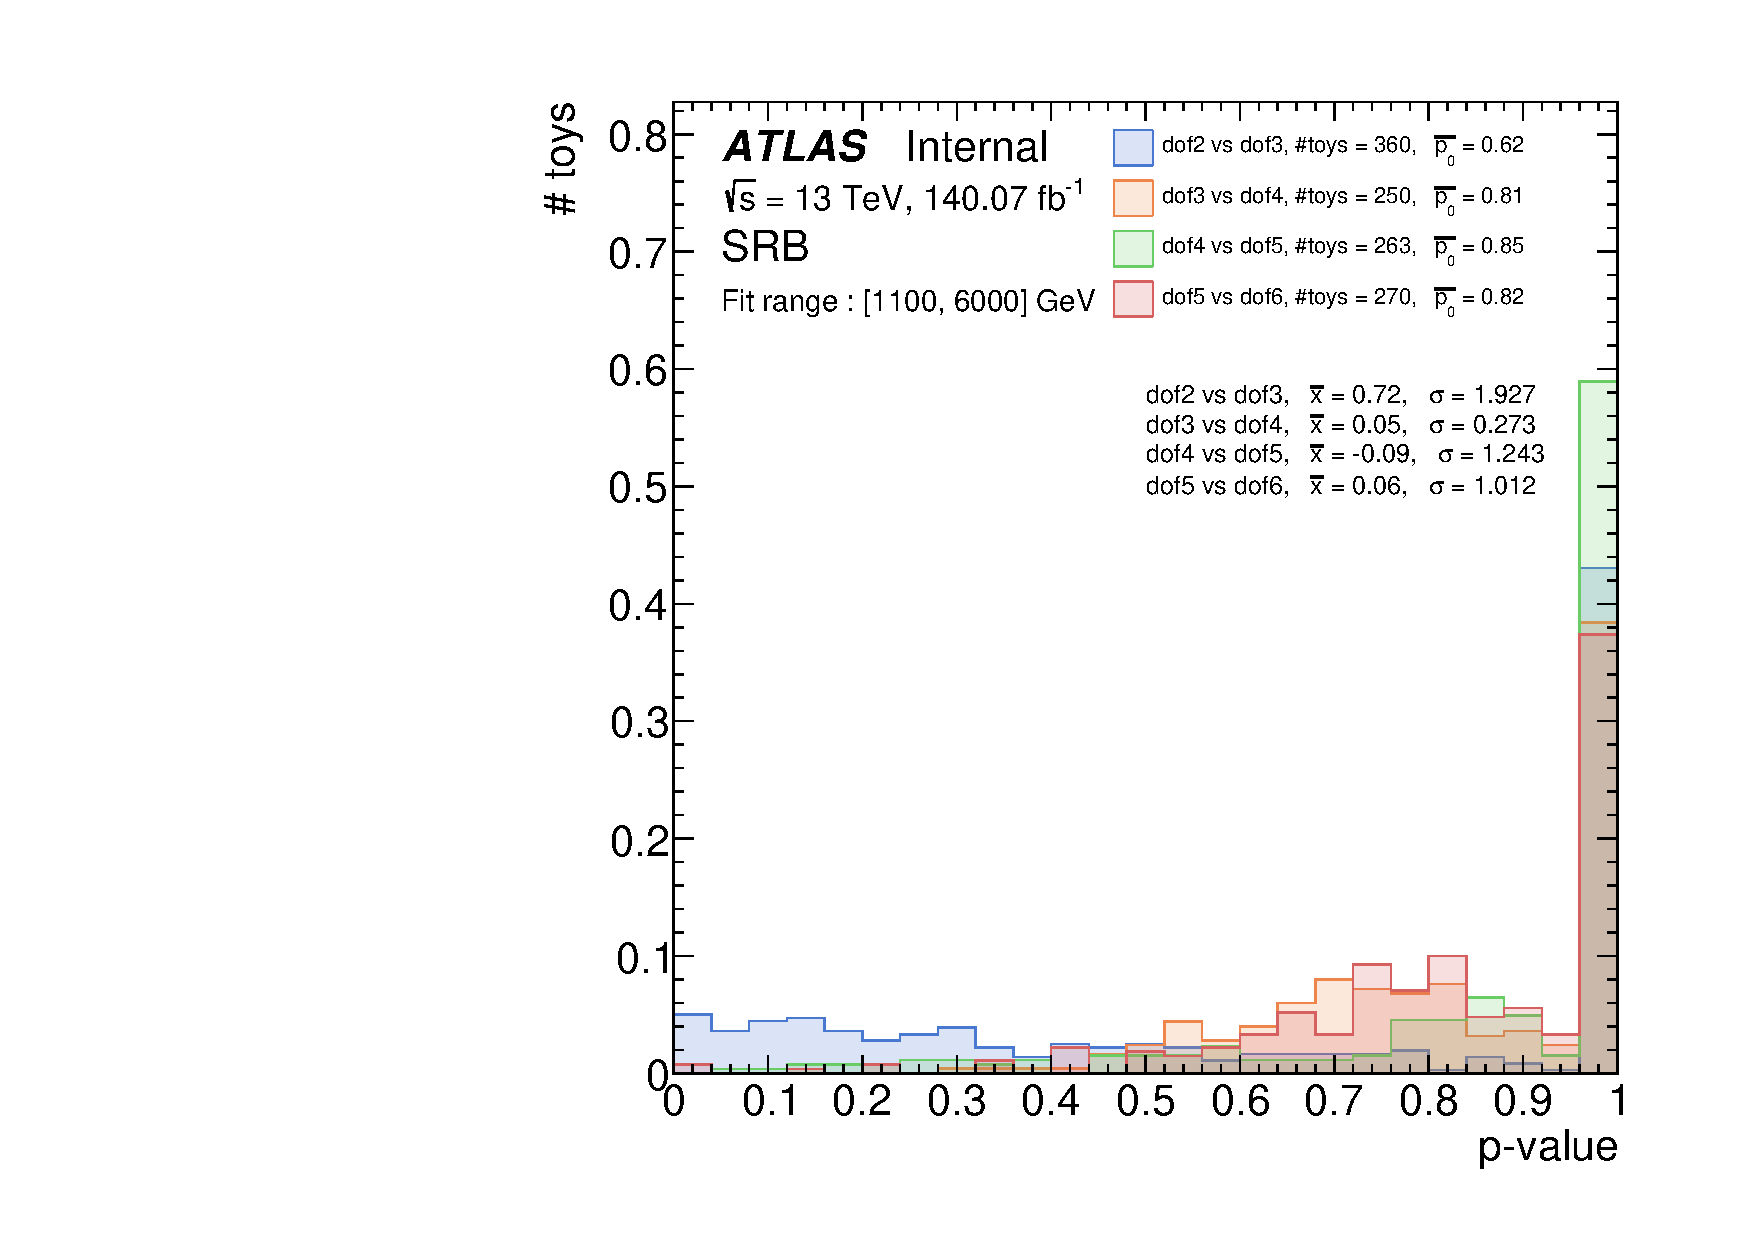
\includegraphics[width=0.8\textwidth]{5_resonances/bkg/modeling/ftest/SRB/can__photonjet_Pythia_jfakeisosmooth__SRB__fvalue_pvalue__range_1100_6000__toys}
        \caption{SRB}
    \end{subfigure}
    \caption{p-value score distribution comparing the performance of the different pair of functions. The reported means and widths correspond to the \(F\)-score distributions, and for each p-value distribution, the average p-value is shown.}
    \label{fig:bkg:modeling:preparation:ftest:ftest_pvalue}
\end{figure}

\Fig{\ref{fig:bkg:modeling:preparation:ftest:chi2ndof}} shows the \(\chisq / \text{ndof}\) distributions for each one of the models for different signal regions computed from toys. It can be seen that all the distributions are centered at \(\sim 1\), meaning that in general all models describe the \ac{BO} distribution correctly. To further compare the different models among them, the \(F\)-score distributions are plotted in \Fig{\ref{fig:bkg:modeling:preparation:ftest:ftest}} for different signal regions, comparing two models at a time. For each pair, the number of toys that converge for both models is shown, as well as the means and widths of the distributions. Likewise, in \Fig{\ref{fig:bkg:modeling:preparation:ftest:ftest_pvalue}} the p-value distribution for the \(F\)-test can be observed, which shows that all the comparison between models lead to \(p(F)\) values very close to 1, meaning that no model fits the distributions better than another. For this reason, no functional model is discarded using the \(F\)-tests.
% Finally, \(F\)-tests computed on Asimov datasets are presented in \Fig{\ref{fig:bkg_modeling:pull}}, where fit pulls are plotted alongside the \(F\)-score and \pzero\ values comparing the different functional models.

% \begin{figure}[htbp]
%     \centering
%     \begin{subfigure}[h]{0.49\linewidth}
%         \centering
%         \includegraphics[width=\textwidth]{figures/background_modeling/ftest/SRB/can__jfakeiso_photonjet_Pythia__SRB__pull__asimov}
%         \caption{SRB}
%         \label{fig:bkg_modeling:pull_SRB}
%     \end{subfigure}
%     \centering
%     \begin{subfigure}[h]{0.49\linewidth}
%         \centering
%         \includegraphics[width=\textwidth]{figures/background_modeling/ftest/SRCT/can__jfakeiso_photonjet_Pythia__SRCT__pull__asimov}
%         \caption{SRCT}
%         \label{fig:bkg_modeling:pull_SRCT}
%     \end{subfigure}
%     \caption{Pulls of the different fits to the MC Asimov datasets using different functional models. The \(F\)-scores and p-values of the pairwise comparison are reported as well. A \pzero-value below 0.05 means that adding the additional parameter significantly improves the fit quality and thus the model with lower parameters should be discarded.}
%     \label{fig:bkg_modeling:pull}
% \end{figure}

% In all regions shown, no significant evidence is found to claim that a model 

% Regarding the \btag region, SRB, it can be noted that the \(F\)-distribution of the comparison between \textit{dof2} and \textit{dof3} is much wider and also has a higher \(F\) mean value. When studying the \pzero\ distribution, it is clearly seen that the blue histogram (\textit{dof2}-vs-\textit{dof3}) primarily populates the \(\pzero\sim 0\) region, apart from the unity value. However, the mean p-value, shown in \Fig{\ref{fig:bkg_modeling:ftest_pvalue_SRB}} indicates that the difference between the models is not sufficient enough to reject the null hypothesis.
% The same situation can be observed when using Asimov datasets, shown in \Fig{\ref{fig:bkg_modeling:pull_SRB}}, in which the \pzero\ values are not small enough to reject any model \(a\) against another one more complex (model \(b\)).

% For the case of SRCT, excepting the \textit{dof2} model which has been excluded from the \ac{SSig} tests, no difference between models is observed as the \(F\)-score distribution is highly concentrated at 0, and the \pzero-value peaking at 1. When comparing the fit pulls from the Asimov fits, no difference whatsoever is seen between the models, again indicating that... \fixmenc{finish this}
%%%%%%%%%%%%%%%%%%%%%%%%%%%%%%%%%%%%%%%%%%%%%%%%%%%%%%%%%%%%%%%%%%%%%%%%%%%%%%%%%%%%%%%%%%%%%%%%%%%%






%%%%%%%%%%%%%%%%%%%%%%%%%%%%%%%%%%%%%%%%%%%%%%%%%%%%%%%%%%%%%%%%%%%%%%%%%%%%%%%%%%%%%%%%%%%%%%%%%%%%
%%%%%%%%%%%%%%%%%%%%%%%%%%%%%%%%%%%%%%%%%%%%%%%%%%%%%%%%%%%%%%%%%%%%%%%%%%%%%%%%%%%%%%%%%%%%%%%%%%%%
%%%%%%%%%%%%%%%%%%%%%%%%%%%%%%%%%%%%%%%%%%%%%%%%%%%%%%%%%%%%%%%%%%%%%%%%%%%%%%%%%%%%%%%%%%%%%%%%%%%%
\subsection{Summary of modeling strategies}
\label{subsec:bkg:modeling:strategy_summary}

Throughout this section different statistical tests have been carried out to determine the optimal fit-range and functional form to model the background distribution in data. These tests have been done for each one of the signal regions considered in the analysis, and also for each signal model.

In the first step, \ac{SSig} tests were performed in order to decide which of these ranges and functions combinations minimise the appearance of any signal when doing \ac{BO} fits. Moreover, the background modeling uncertainty results from this test, meaning that using the combination that lead to the lowest \ac{SSig}, will also influence the final uncertainties when performing the search on data. For each fit-range, rankings of the functional models are built and are all passed through the \ac{SI} and \(F\)-tests. The former checks if the function is able to capture all the injected signal to the background, and the second tests if by adding another \ac{dof} to the function a significant improvement on the fits is seen.

As discussed in \Sect{\ref{sec:strategy:stat_treatment:fits_results}}, two types of interpretations are studied. In the \ac{BO} interpretation, the fits are done to data with a \ac{BO} model, that is, the signal strenght in \Eqn{\ref{eq:strategy:stat_treatment:stat_model:likelihood}} is fixed at 0 and all the nuisance parameters are fitted. These fits are performed in regions SR, SRB and SRC, using the functions and ranges given in \Tab{\ref{tab:bkg:modeling:strategy_modeling:summary}}. On the other hand, for the \ac{SB} interpretation the signal strength \(\mu\) is allowed to float and the yielded signal is quantified. The fits to data are then performed with a \ac{SB} model, where the signal component is a \ac{PDF2} and the background function differs for each signal model and signal region. In \Tab{\ref{tab:bkg:modeling:strategy_modeling:summary}}, a summary of the functional forms and the fit-ranges for each signal model and region are displayed.


\begin{table}[ht!]
    \centering
    \caption{Summary of fit strategies for each analysis region and signal model. The table shows the functional form used, as well as the \myj fit-range in GeV. The last column indicates if the fit is performed simultaneously for the SRC, SRB and SRL regions, in case each one of them are used for the interpretation/model.}
    \resizebox{\linewidth}{!}{
        \begin{tabular}{lccccc}
            \toprule
                                & Inclusive SR                      & SRL                               & SRC                               & SRB                               & \begin{tabular}{@{}c@{}} Do simult. \\SRC+SRB+SRL? \end{tabular}\\
            \midrule
            \ac{BO}             & \textit{dof2}, \([1000,8000]\)    & \textit{dof2}, \([1200,8000]\)    & \textit{dof4}, \([1100,7000]\)    & \textit{dof2}, \([1100,6000]\)    & No                      \\
            \midrule
            Gaussians           & \textit{dof3}, \([1200,8000]\)    & \textit{dof3}, \([1500,8000]\)    & \textit{dof4}, \([1000,7000]\)    & \textit{dof5}, \([900,7000]\)     & No                      \\
            \ac{QBH}            & \textit{dof5}, \([1000,8000]\)    & -                                 & -                                 & -                                 & -                       \\
            \ac{EQ}, \qstar     & \textit{dof2}, \([1000,8000]\)    & -                                 & -                                 & -                                 & -                       \\
            \ac{EQ}, \cstar     & -                                 & \textit{dof2}, \([1200,8000]\)    & \textit{dof4}, \([1100,7000]\)    & \textit{dof2}, \([1100,6000]\)    & Yes                     \\
            \ac{EQ}, \bstar     & -                                 & -                                 & -                                 & \textit{dof2}, \([1100,6000]\)    & -                       \\
            \bottomrule
        \end{tabular}
    }
    \label{tab:bkg:modeling:strategy_modeling:summary}
\end{table}


%%%%%%%%%%%%%%%%%%%%%%%%%%%%%%%%%%%%%%%%%%%%%%%%%%%%%%%%%%%%%%%%%%%%%%%%%%%%%%%%%%%%%%%%%%%%%%%%%%%%
%%%%%%%%%%%%%%%%%%%%%%%%%%%%%%%%%%%%%%%%%%%%%%%%%%%%%%%%%%%%%%%%%%%%%%%%%%%%%%%%%%%%%%%%%%%%%%%%%%%%
%%%%%%%%%%%%%%%%%%%%%%%%%%%%%%%%%%%%%%%%%%%%%%%%%%%%%%%%%%%%%%%%%%%%%%%%%%%%%%%%%%%%%%%%%%%%%%%%%%%%